\documentclass[twoside,11pt]{article}

% Any additional packages needed should be included after jmlr2e.
% Note that jmlr2e.sty includes epsfig, amssymb, natbib and graphicx,
% and defines many common macros, such as 'proof' and 'example'.
%
% It also sets the bibliographystyle to plainnat; for more information on
% natbib citation styles, see the natbib documentation, a copy of which
% is archived at http://www.jmlr.org/format/natbib.png

\usepackage{jmlr2e}
\usepackage{setspace}
%\singlespacing
\onehalfspacing % Line space

\setlength{\marginparwidth}{2.5cm} % For notes in margin, can be delete for final version.

% Definitions of handy macros can go here

\newcommand{\dataset}{{\cal D}}
\newcommand{\fracpartial}[2]{\frac{\partial #1}{\partial  #2}}
\DeclareMathOperator{\Tr}{Tr}

% Heading arguments are {volume}{year}{pages}{date submitted}{date published}{paper id}{author-full-names}

\jmlrheading{1}{2018}{1-48}{4/00}{10/00}{meila00a}{Kungang Zhang, Anh T. Bui, and Daniel W. Apley}

\definechangesauthor[name={Per cusse}, color=brown]{Kungang}
\definechangesauthor[name={Per cusse}, color=orange]{Anh}
\definechangesauthor[name={Per cusse}, color=red]{Apley}
% \setremarkmarkup{(#2)}

% Short headings should be running head and authors last names

\ShortHeadings{Zhang, Bui, and Apley}{}
\firstpageno{1}

\begin{document}

\title{Concept Drift Monitoring and Diagnostics of Supervised Learning Models via Score Functions}

\author{\name Kungang Zhang \email zkg@u.northwestern.edu \\
	\name Anh T.\ Bui \email buiat2@vcu.edu \\
	\name Daniel W.\ Apley \email apley@northwestern.edu \\
       \addr Department of Industrial Engineering and Management Sciences\\
       Northwestern University\\
       Evanston, IL 60208-3119, USA\\
       Department of Statistical Sciences and Operations Research\\ 
       Virginia Commonwealth University\\
       Richmond, VA 23284-3083, USA}

\editor{EDITOR NAMES}
% Author guide: http://www.jmlr.org/format/authors-guide.html
\maketitle
% What is the name of our method? IKPCA or IKM?
% Ans: Think about it constantly.
% Whether we should put number in the visualization?
% Ans: Yes.
% Whether should I put true variation sources and 3-D visualization of PCA scores for every 2-dimensional manifold case?
% Ans: Maybe not 3D but we should put original variation sources there.
% How to present 3D face data set result?
% Ans: Think about it.
% Whether I should describe in details the data pre- and post-processing (linear PCA and choosing asymmetric autoencoder)?
% Ans: Yes, but it should be simple. Don't put 95% and 99% in the paper but keep record of it in case reviewer asks.
% For the connection with GPLVM and other method, whether I should put detailed mathematic formula in appendix or in the discussion part of the paper?
% Ans: Yes, if only requires 3-4 math formula, we should put them in the paper.
% About visualization and presentation contest.
% Ans: Not recommend it.
% Size of data points.

% More work:
% I need to look into literature and find another real data set people used for manifold learning and prove that our method works better than other method on this data set.

\begin{abstract}%   <- trailing '%' for backward compatibility of .sty file
\replaced[id=Anh, comment={}]{Supervised learning models}{Machine learning models} are widely adapted in many applications, as in medicine, finance, technology, and manufacturing, to automate business process or decision-making. The dataset collected for the purpose of training models \replaced[id=Kungang, comment={}]{could be}{is} either not stationary or distributed differently from dataset for testing or decision-making \deleted[id=Anh, comment={}]{, as known as dataset drift}. This violates the assumption of stationarity in training \replaced[id=Kungang, comment={}]{, potentially rendering}{or renders} fitted models obsolete in testing \added[id=Kungang, comment={}]{, as known as concept drift}. In this study, those methods in literatures designed to address various aspects of problems of \replaced[id=Anh, comment={}]{concept drift}{dataset drift} are hierarchically organized in terms of challenges they are trying to attack (i.e. detection or adaptation) and types of drifts. Then, in the context of \replaced[id=Kungang, comment={}]{supervised learning}{predictive} models, the problem of concept drift which refers to the changes over time of relationship between $\bm {X}$ and $Y$ is investigated and a comprehensive and computationally light framework of detecting, monitoring, and diagnosing concept drift is demonstrated. Specifically, we propose to apply \replaced[id=Anh, comment={}]{a powerful statistical process control (SPC) technique, multivariate EWMA chart}{exponentially weighted moving average (EWMA) and Hotelling $T^2$ multi-variate control chart} on the score function for detecting and monitoring concept drift \deleted[id=Anh, comment={}]{in Phase-I and Phase-II respectively}; \replaced[id=Kungang, comment={}]{the diagnosis method proposed can}{after rescaling score vectors (realization of the score function), we} trace the origin of concept drift to specific covariates to provide an interpretation. \deleted[id=Anh, comment={}]{This is the first time in the concept drift literatures that a score-based method is developed.} The advantages include a portability for online detection with \replaced[id=Kungang, comment={}]{any parametric supervised learning}{different} models, shorter delay in detection, and higher sensitivity, \replaced[id=Kungang, comment={}]{as shown in experiments with various models on simulated and real datasets.}{In order to demonstrate them on linear and nonlinear models, linear, logistic, multinomial, Poisson regression, and neural network are tested on many simulated datasets.} \replaced[id=Kungang, comment={}]{The impressive performance of early detection and interpretability demonstrate the superiority of the proposed method over current popular ones.}{Two real datasets are used to support the conclusions from simulations.} \deleted[id=Anh, comment={}]{We also discuss some related results from econometric literatures and draw a connection between our and their methods.} 
\end{abstract}

%Instead of being collected once, data is usually collected in order of time or streamingly, and may be processed sequentially, because of the abundance of data and limited space of memory. 

\begin{keywords} 	
  Concept Drift, Score Function, Control Chart, Streaming Data, Predictive Model
\end{keywords}

\section{Introduction}
% General dataset shift problem.
%Introducing the definition of concept drift and some mathematical notation for it. Also, justify the investigation of concept drift in training and testing.

%In current digital age, data generation and collection are largely automated. To understand data and mine insights from it, many models are developed, i.e. supervised and unsupervised learning models. Training a model usually requires a collection of historical data, which is assumed distributed approximately as the true data distribution. Then some objective function depending on historical data is optimized to determine the parameters or structure of models. How to implement this training process depends on the size of datasets and how data are collected. For example,
%
%\begin{itemize}
%\item
%\textit{Batch and Offline Learning}
%In applications with small datasets and data are available before training starts, batch-learning and offline-learning can be applied, meaning the objective function depends on all training data and the model is obtained by finding the optimal solution of this objective function.
% \item
% \textit{Mini-Batch and Offline Learning}
%when dataset is large (cannot fit into memory) and data are available before training, models can be trained sequentially by feeding a subset of data one at a time (i.e. mini-batch or SGD), still offline learning because data points can be used as many times as possible.
% \item
% \textit{Online Learning} 
%When data are collected continuously, entire historical data cannot be stored and can only be used once, and models are needed since the early time of data collection, online learning can be used to update the model using data points one-by-one until time horizon.
%\end{itemize}
%
%Correspondingly, applying models obtained from the above three training modes is also different: For \textit{Batch} and \textit{Mini-Batch} and \textit{Offline Learning}, models are used for all future incoming data, until retraining is requested. For \textit{Online Learning}, models are used and updated constantly. 
%
%In real applications, data are often generated in a dynamic environment, meaning the distributions of the data is changing over time. The impact of such temporally dependent data distribution on model training and applying is also different based on training modes. For Offline Learning, the unstationary distribution of training data jeopardizes the quality of obtained model, because the trained model is based on a mixture of older and newer distribution; the unstationary distribution of testing data may invalidate the trained model. For Online Learning, the temporal dependence of data distribution can somehow be captured by the updating mechanism, and the performance degradation can be mitigated, however, usually at the expense of more computation in maintaining an up-to-date model. 
%
%Many sophisticated algorithms has been invented to address problems of dataset drift. They can be categorized into detection and handling methods, in terms of goals of applying the algorithm, or into concept/covariate/prior drift, in terms of types of drift the algorithm targets on. For detection methods, the difference (latency) between the time real drift happening and the detection and false positive rate are primary focuses. The early detection of drift after the real drift happens can lead to more responsive adjustment or retraining of the model and thus benefit the performance of the algorithm. 
%
%For handling methods, 
%
%
%
%One brutal force method that borrows advantages from all training modes is periodically retraining a new model using recent historical data. This involves drift detection and drift updating method. The drift detection 
%
%
%
%
%However, such online learning sometimes are computational expensive and unnecessary, because model needs to be updated every now and then no matter whether there is a significant temporal dependency. 


%Concept drift in stochastic gradient descent
%
Predictive (supervised learning) models are widely used in many applications, {such as} drug testing~(\cite{fong2015change}), credit risk rate prediction~(\cite{im2012time}), spam filtering~(\cite{carmona2010gnusmail}), recommendation system~(\cite{koren2009collaborative}), production quality control~(\cite{bui2018monitoring}), {(more examples in~(\cite{vzliobaite2016overview}))}. In those applications, predictive models are trained on historical data, which typically include {$n$} observations of {$\{ (\bm {x}_i, y_i)|, i=1,2,\cdots,n$\}}. {Then, those models can make prediction of the response variable $y^*$ given a future predictor variable $\bm {x}^*$}, where {$\bm {x}_i \in \mathbb{R}^{p}$ and $y_i \in \mathbb{R}$ are the covariates and response variable in the $i$th observation respectively}\footnote{\replaced[id=Kungang, comment={}]{The case with scale response can}{Can} easily be extended to vector response variable $\bm {y}_i$.}. The assumption behind this prediction is that the distribution of {$ {Y}$} given {$\bm {X}$}, {$P (Y| \bm {X}, \bm { \theta})$}, is stationary over time, {where $P (Y| \bm {X}, \bm { \theta})$ is a parametric approximation to $P (Y| \bm {X})$ with $\bm { \theta}$ as the vector of parameters}. In this case, we think of the data are generated in \replaced[id=Anh, comment={}]{stationary}{static} environment \added[id=Anh, comment={}]{, where the stationarity refers to the conditional distribution, $P(Y|\bm {X})$}. However, {in many cases, the} conditional distribution $P (Y| \bm {X})$ may change over time (aka concept drift~(\cite{moreno2012unifying})). \replaced[id=Anh, comment={}]{Concept drift}{Drift of joint distribution} of observations $ (\bm {x}_i, y_i)$ in training (historical) and testing (future) can both degrade performance of predictive models: in training, concept drifts would invalidate the assumption of data being stationary; while in testing concept drifts quantitatively change the original relation between the predictor $\bm {X}$ and $Y$, different from the one captured by trained models. \footnote{This should not be confused with the case called ``covariate drift'', where {$P (Y| \bm {X}, \bm { \theta})$ doesn't change but $P (\bm {X})$ changes.} However, the effect of ``covariate drift'' on detection of ``concept drift'' in our method will be formally discussed later.} \deleted[id=Anh, comment={}]{The change in $P (Y|\bm {X}, \bm { \theta})$ can happen in training and serving models.} To ensure the quality of trained models, training datasets should be explored to \replaced[id=Kungang, comment={}]{potentially rule out}{prevent potential} concept drifts \added[id=Kungang, comment={}]{as much as possible, through so-called retrospective analysis}. In testing or serving models, the performance should be monitored to alarm \added[id=Kungang, comment={}]{or diagnose} potential concept drifts. 

%\subsection{Existing Works}
%Quick review about structure change appears in econometric literatures; the limitation of focusing on GLM; formal hypothesis testing; restriction in using the monitoring scheme. No non-parametric models.
\added[id=Kungang, comment={}]{Concept drift is fairly common in practical applications. For example, in spam filtering, machine learning models can use features like words, spelling, and addresses to determine whether an email comes from a suspicious source. However, when spammers find their outgoing emails are blocked, they can invent new templates of emails trying to bypass the spam checking. Or some emails previously not regarded as spams become ones after a while. 
%Give a deeper explanation of concept drifts. Pinpoint the objective of a good algorithm for handling concept drift. Differentiate our context from those using variables of concept to identify concept drift.
These phenomena in one case can originate from hidden effects or contexts not captured by machine learning models. When hidden effects don't change, the current model can approximate relationship between covariates and responses, if well-trained and validated. However, after the context drifts, the same model may have very poor predictability based on input variables. Battling against performance degradation resulting from concept drift is especially important in streaming data setting. Considering large amount of data and big scale of models, a good method for solving concept drift problems should be able to handle different kinds of drifts very fast without requiring too many data points. Also, to quickly pinpoint specific features or covariates contributing to a drift, a good method should also provide interpretive guidance.}

\deleted[id=Anh, comment={}]{The concept drift problem have emerged in different fields, including machine learning~(cite{gama2004learning}), statistics~(cite{brown1975techniques}), and econometrics~(cite{kuan1995generalized}). Classification problems are especially interested in by machine learning communities.} Many complex models, like ensemble methods~(\cite{wang2003mining}), neural networks~(\cite{calandra2012learning}), and other non-parametric methods~(\cite{dos2016fast}, \cite{frias2015online}) are developed to detect and adapt concept drifts. Most state-of-art methods are designed based on classification error or some metrics derived from it~(\cite{barros2018large}, \cite{ross2012exponentially}, \cite{gonccalves2014comparative}). \deleted[id=Kungang, comment={}]{In fields of statistics and econometrics, score-based testing methods~(cite{zeileis2005unified}) are developed for both regression and classification problems to handle changes of parameters, where the score function is defined as gradient of cost function (e.g., negative log-likelihood) of single observation.} \added[id=Kungang, comment={}]{In this paper, we will discuss the limitation of using error-based methods, like missing potential concept drifts and opportunities of improving models (as illustrated in Figure~\ref{fig:logi_err_rate_unch}) and so on. To overcome those problems, we choose to monitor stochastic score function, defined as the gradient of log-likelihood.} As no direct \added[id=Kungang, comment={}]{and quantitative} comparison have been made on those methods before, this study bridges the gap \deleted[id=Kungang, comment={}]{across the fields} by a) justifying the merits of score-based methods from both theoretical and empirical perspectives; and b) developing a comprehensive framework to detect, monitor, \added[id=Kungang, comment={}]{and diagnose} concept drift using the state-of-art multi-variate SPC method based on score function. Extensive simulations and two case-studies based on real datasets have shown that score-based method is: 
\begin{enumerate}[1)]
\item
\textit{necessary to monitor concept drift, because concept drift doesn't necessarily result in change in error, but sufficiently changes the mean of score-based metrics to be non-zero, so that it opens up the possibility of any type of mean-change monitoring method;}
\item
\textit{more sensitive, thus less delayed in detecting concept drifts than error-based methods;}
\item
\textit{more interpretable of origins of concept drift;}
\item
\textit{computationally cheap and generally applicable for all parametric models.}
\end{enumerate}

%As mentioned, the temporarily dependent parametric models are investigated in both econometrics and machine learning, and surprisingly there is no cross-citation between two fields. In econometrics, generalized linear models (GLM) are mostly investigated and formal hypothesis testing under the framework of the M-fluctuation tests are devised to signal the alternatives hypothesis. However, the tests developed in those papers are either based on cumulative sum or moving sum with equal weights, without much discussion about changing weights, such as EWMA. In the contrast, in machine learning and pattern recognition papers, the statistics to be monitored and methods used to monitoring them are designed based on error rate or residuals of models~(\cite{barros2018large}, \cite{wang2015concept}), which sometimes can be looked as a special case of score-based M-fluctuation tests (because the first element of the score function is the residual of generalized linear models). However, many weighting schemes, including EWMA, are proposed to better fit different kinds of drifts, for example abrupt v.s. gradual drift. Some of them are very computational expensive. In this study, we are combining ideas and techniques from both fields to achieve a flexible and computation-cheap method, which can be easily integrated into any existing machine learning system using models like generalized linear models. The diagnostic component we developed exemplifies the advantage of using score-based instead of residual-based statistics, and simulated and real datasets show its competitive performance in early detection. We want to stress that this paper is focusing on developing an intuitive and useful method for data exploration and concept drift or parameter instability online detection. 

%Adapt score-based methods to concept drift problems. Using EWMA monitoring scheme. We develop a diagnostic method. In literatures from previous two fields, there is a lack of investigation on this one. This method can only be applied onto score functions. It is very cheap because the score is usually by-production of making prediction and fine-tuning or training, and . Our method is computationally cheap, because it is a by-product. We extend our method to non-parametric model like neural network. 

\deleted[id=Kungang, comment={}]{In this study, we develop a method of detecting concept drift .} The score-based method \replaced[id=Kungang, comment={}]{monitors}{is adapted to monitor} sample score vectors\footnote{In the paper, we use ``the score function" for \replaced[id=Kungang, comment={}]{the gradient of log-likelihood as a function}{the function} and use ``sample score vectors" for evaluation of the score function given specific data $(\bm {x}_i,y_i)$ and value of parameters.} (realizations of the score function), using multivariate exponentially weighted moving average (MEWMA) control charts~(\cite{montgomery2007introduction}). Because this method requires the score function, we focus on parametric models. {We also develop a visualization procedure, using (univariate) exponentially weighed moving average (EWMA) control charts to monitor each component of sample score vectors, for diagnosing the nature of detected drifts.} 

The several advantages for this method are detailed as following. First, the sample score vectors can be automatically produced in prediction step and stochastic gradient \added[id=Kungang, comment={Comment: Here, the reason I am using SGD instead of SG is because I want to emphasize that the method we developed can be used along with SGD, even though we are not updating our model each step. The monitoring can still make sense when we want to calculate a batch of stochastic gradients and do the updating using the batch mean of score function}]{descent (SGD)} as the derivative of the marginal log-likelihood {$\nabla _{\bm { \theta}} \log(P (y_i|\bm {x}_i, \bm { \theta}))$} which is widely used in the cost function in training predictive models. A machine learning model can be finely tuned using SGD after collecting all data; or it can be tuned online if data generating process is stationary. In other words, obtaining sample score vectors from offline or online learning during fine tuning (or prediction) requires very little extra calculation, so that this method can be easily integrated into existing systems as a component of data exploration and model performance monitoring. Second, the MEWMA scheme \replaced[id=Kungang, comment={}]{can detect the change of vectors in a direction invariant manner and the exponentially decayed weights smoothly distributed higher weights on recent data samples over earlier ones without relying too much on a single data point. The value of decaying parameters depends on specific applications and a good choice can find balance between false-alarm rate and detection speed.}{puts more weights on recent data so that it has better performance in early detection comparing against CUSUM and MOSUM in detecting small drifts}. Third, this score-based methods is very general and can be applied onto any models which can obtain derivatives with respect to parameters, like generalized linear model or neural network. In contrast to those \textit{ad-hoc} \added[id=Kungang, comment={}]{error-based} metrics like precision and recall, using score function is more general \added[id=Kungang, comment={}]{for parametric models}. The score function has the same dimension as the number of parameters. The information contained is multidimensional, so that it can provide interpretation for the concept drift. We demonstrate our methods on linear, logistic, multinomial, and Poisson regression.

%\subsection{Origins and Applications of Concept Drift}
%Give two real examples of concept drift
\deleted[id=Kungang, comment={}]{Besides interests from mathematical perspective, concept drift is fairly common in practical applications. For example, in spam filtering, machine learning models can use features like words, spelling, and addresses to determine whether an email comes from a suspicious source. However, when spammers find their outgoing emails are blocked, they can invent new templates of emails trying to bypass the spam checking. Or some emails previously not regarded as spams become ones after a while. Another example is predicting efficacy of antibiotics using predictive models. With more usage of a certain antibiotics, bacterias become more resistant offsetting the efficacy, up to a point when it becomes virtually useless.
%Give a deeper explanation of concept drifts. Pinpoint the objective of a good algorithm for handling concept drift. Differentiate our context from those using variables of concept to identify concept drift.
In other cases, it can also be captured by some context variables which, instead of being explicitly used as covariates in training, are converted to weights to select historical data having similar context for training~(cite{barakat2018context}). The main difference in the two settings is that the former assumes no explicit knowledge in concept drift, while in the later case concept drifts are identified given candidate context variables. We clarify that this paper focuses on the former setting, which no prior knowledge of concept drift is required. These phenomena in one case can originate from hidden effects or contexts not captured by machine learning models. When hidden effects don't change, the current model can approximate relationship between covariates and responses as well as the one being trained. However, after the context drifts, the same model may have very poor predictability based on input variables. Battling against performance degradation resulting from concept drift is especially important in streaming data setting. Considering large amount of data and big scale of models, a good method for solving concept drift problems should be able to handle different kinds of drift very fast without requiring too many data points. Also, to quickly pinpoint specific features or covariates contributing to a drift, a good method should also provide interpretive guidance.}

%%Pinpoint the problems in the existing methods.
%
%As mentioned, the temporarily dependent parametric models are investigated in both econometrics and machine learning, and surprisingly there is no cross-citation between two fields. In econometrics, generalized linear models (GLM) are mostly investigated and formal hypothesis testing under the framework of the M-fluctuation tests are devised to signal the alternatives hypothesis. However, the tests developed in those papers are either based on cumulative sum or moving sum with equal weights, without much discussion about changing weights, such as EWMA. In the contrast, in machine learning and pattern recognition papers, the statistics to be monitored and methods used to monitoring them are designed based on error rate or residuals of models~(\cite{barros2018large}, \cite{wang2015concept}), which sometimes can be looked as a special case of score-based M-fluctuation tests (because the first element of the score function is the residual of generalized linear models). However, many weighting schemes, including EWMA, are proposed to better fit different kinds of drifts, for example abrupt v.s. gradual drift. Some of them are very computational expensive. In this study, we are combining ideas and techniques from both fields to achieve a flexible and computation-cheap method, which can be easily integrated into any existing machine learning system using models like generalized linear models. The diagnostic component we developed exemplifies the advantage of using score-based instead of residual-based statistics, and simulated and real datasets show its competitive performance in early detection. We want to stress that this paper is focusing on developing an intuitive and useful method for data exploration and concept drift or parameter instability online detection. 
%
%To overcome concept drift, many methods have been proposed to handle concept drifts or parameter instability, which can be categorized into two classes: 1) concept drift handling methods which are mostly coming from machine learning field; 2) concept drift detection methods which are developed in both machine learning and econometrics. The concept drift handling methods mainly focus on the performance of machine learning models, without too much care about detection and diagnosis. To maintain a good prediction accuracy (classification or regression), models are updated online while new data points are collected, a paradigm usually called online or incremental learning. Among them the ensemble methods are the most popular. Those methods have an advantage of continuity, without a cold start once a good model has been trained. And because they have some kind of forgetting mechanism, they automatically track new concepts. However, because, each time a new data point or data batch coming in, they need to update the ensemble of models or add new models into the ensemble no matter whether concept drift happens, those methods can waste lots of computation budget. This disadvantage and the complexity of tuning many parameters are probably the reason of the lack of popularity of those methods in industry. The other category of methods is aimed to detect concept drifts with relative cheap computation cost. Examples include DDM, EDDM, Linear-4-rate, ...... from machine learning field, or M-fluctuation tests from econometrics. Those methods require monitoring some statistics for potential concept drifts. When the statistics passes a threshold or a boundary function carefully designed, an alarm is triggered and extra intervention would follow. Even though those methods look less automatic than those from the first category, it can provide more information and earlier detection about system being monitored. Because of not involving online updating models, those kind of methods is far cheaper. However, nothing prevents a user to apply methods from both categories to a problem to incorporate advantages from both sides. In this study, we develop a method belonging to the second category. 

%Among methods from the second category, those parametric methods mostly monitor some model performance metrics (like cumulative prediction accuracy or other \textit{ad hoc} metrics) as a signal for concept drift~(\cite{barros2018large}). However, there are several issues related to these methods. First, they are usually developed for the sake of predictive performance without providing interpretive diagnosis on the origin of concept drifts. Second, the stationarity of dataset in training supervised learning models are not justified. Usually, data collected over a period of time are treated i.i.d. without justification. Third, some monitoring methods~(\cite{wang2015concept}) are designed to detect drifts in hand-crafted statistics (performance metrics) related to the predictive model (limited to certain problems).

%However, there are several shortcomings related to them: those methods usually involve thresholding parameters requiring hand-tuning and hand-crafted performance metrics lacking of statistic or probability justification; the concept drift can happen without changing those metrics; and there is few method providing diagnostic information for the concept drift detected~\cite{demvsar2018detecting}.
%For example, the default probability of credit card holders given their information may be quite different before and after economic crisis; or the prediction of the number of hourly bike rental is changing based on increasing popularity of the concept of bike sharing, besides the effect of \replaced[id=Anh, comment={}]{covariates}{covariates} like weather, working day, etc. 
% Need to find the drawback of existing method to set a backdrop for showcasing advantages of our method in the next paragraph.
%Previous methods, several issues relate to these methods. First, they are usually developed for the sake of predictive performance without providing interpretive diagnosis on the starting time and covariate origin of drifts. Second, re-training models sometimes can be quite expensive both in terms of computation and data collection. Third, the stationarity of dataset in training supervised learning models are not justified. Other monitoring methods~\cite{wang2015concept} are designed to detect drifts in hand-crafted statistics related to the predictive model, specific to certain problems. 
%Online learning~\cite{?} methods are used to train a model in timely manner so that the model can adaptively capture the correspondence relation between covariates and responses, (e.g. ensemble model~\cite{elwell2011incremental}, re-training model using moving window~\cite{?}, etc.). 

%Highlight the advantages of our methods and summarize the content of later sections.
%Our method is simple and universal to all parametric supervised learning models. It 
Our method provides quantitative guidance on when the model should be updated {on occurrence of a drift. It can also justify the stationarity assumption when fitting models, \added[id=Kungang, comment={}]{through retrospective analysis}.} {In addition, the approach can provide insights about the} nature of the drift, {which can be} highly valuable in {many applications (e.g., business, insurance, and health care, etc.)}, and in turn maintain high performance of models. In big and streaming data {contexts,} this monitoring method is computationally cheap thus fast because sample score vectors are by-products of SGD or partially calculated in prediction step. {In example and discussion section, simulated and real datasets (credit risk and city bike sharing datasets) for both classification and regression will be studied as demonstration.} 
\added[id=Kungang, comment={}]{Simulated datasets are also used to illustrate the advantages of score-based over error-based methods, in terms of detection speed and interpretability, under circumstances of abrupt/gradual concept drifts and with/without multi-colinearity. Overall, we show that monitoring score instead of error would give overall better performance and understanding in handling concept drift with very little extra cost.}
\deleted[id=Anh, comment={}]{Four parametric models, linear, logistic, multinomial, and Poisson regression, are used as examples to investigate this method. For non-parametric or semi-parametric model, we investigate multi-layer perceptron (MLP) as an example. The MEWMA can be used to track overall concept drift with special treatment to handle models with a large amount of parameters, like MLP. For linear and mildly nonlinear models, it can also track concept drift of individual covariates. Simulated datasets are carefully designed to demonstrate that, for linear models, component-wise concept drift can be completely recovered even with multi-collinearity; for nonlinear models like logistic regression, our method can still be practically useful because, when concept drift happens and a model being trained is mostly affected (will be clarified later), we can linearize the decoupling matrix to get a good approximation and obtain decoupled concept drifts for covariates. {Furthermore, other methods monitoring EWMA of prediction residual or error rate are compared with our method showing that monitoring the score function can provide earlier detection.} Experimental studies on real datasets of credit risk and bike sharing prove that tracking sample score vectors is better than simply monitoring prediction error or residual and offers more interpretive results for improving performance of predictive models.}

%The application of this method for finite sample biased estimators is also discussed (ridge regression or lasso regression).

\section{Related Works}
Concept drift problem is getting more attention recently, because in real applications data are often generated in a dynamic environment, meaning the distributions of the data is changing over time. The impact of such temporally dependent data distribution on model training and prediction is different based on different kinds of drift. In the literatures of dataset drift, the definition are not always consistent, but the most common one is used in this study, as in~(\cite{moreno2012unifying}). In general, any temporal dependency of joint distribution $P(\bm {X}, Y)$ is called dataset drift. After decomposing the joint distribution into the form $P(\bm{X}, Y) = P(Y|\bm{X})P(\bm {X})=P(\bm {X}| {Y})P(Y)$, more precise treatment can be applied according to different kinds of drifts. To unify terminology, it is necessary to briefly review relevant existing literatures of different types of drift, in terms of goals and methodologies. 

In some literatures from econometrics, terms like ``structural change" and ``parameter instability" are used to describe a phenomenon in which the parameters of some regression models changes in historical (retrospective) or future data (forward-looking)~(\cite{zeileis2005unified}). A unified framework called the generalized ``M-fluctuation" test is designed to test against the null hypothesis, which assumes no change in parameters. The M-fluctuation test encompasses many different testing statistics sharing the same functional form and all based on score function, which is defined as derivative with respect to parameters of a given objective function~(\cite{zeileis2007generalized}). The advantage of the M-fluctuation test is that its asymptotic properties can be derived analytically using functional central limited theorem, which then can be used to derive theoretical critical value or boundary functions. Some popular test statistics \added[id=Kungang, comment={}]{in econometrics literatures} include CUSUM and MOSUM~(\cite{xia2009monitoring}). Those theoretical properties work for generalized linear models under certain technical assumptions, and the test statistics thus also have some restriction. For example, no EWMA form of test statistics are discussed in those literatures, but EWMA method \added[id=Kungang, comment={Comment: Since one of our main interests is the detection speed, so that I think EWMA is better than CUSUM and MOSUM. However, of course, a good performance depends on how to choose EWMA parameter, which deserves another research project on itself.}]{can achieve earlier detection and} is very popular in quality control and pattern recognition to handle streaming data~(\cite{ross2012exponentially}). And the test statistics they designed usually involve cumulative sum of score functions, which can be slow in detecting and tracking online structure changes. \added[id=Kungang, comment={}]{Another restriction is that those literatures mainly focus on simple model, like generalized linear models, without touching more nonlinear ones, like neural networks.} 

%In concept drift, people focus on errors or residuals which lose lots of information. Computational expensive. 
In contrast, literatures of concept drifts use more flexible methods and the ``drifts" to be detected are not restricted to some formal hypothesis testing. Methods, proposed in concept drift literatures, can be categorized into two classes~(\cite{tsymbal2004problem}): 1) concept drift handling methods; 2) concept drift detection methods. 

The concept drift handling methods mainly focus on the performance of machine learning models, without too much care about detection and diagnosis. To maintain a good prediction accuracy (classification or regression), models are updated online while new data points are collected, a paradigm usually called online or incremental learning. Among them the ensemble methods are the most popular. \added[id=Kungang, comment={}]{Those methods have an advantage of continuity, without a cold start once a good model has been trained. And because they have some kind of forgetting mechanism, they automatically track new concepts. However, because, each time a new data point or data batch coming in, they need to update the ensemble of models or add new models into the ensemble no matter whether concept drift happens, those methods can waste lots of computation budget. This disadvantage and the complexity of parameter tuning are probably the reason of the lack of popularity of those methods in industry.} \added[id=Kungang, comment={}]{Another type of method in the concept drift handling methods is incremental learning. One common property of incremental learning is that it usually involves only one model and the model is maintained updated to incorporate current state of concept. Such learning algorithms are usually specifically designed for a subset of models, so that the applications of them are restricted.} \added[id=Kungang, comment={}]{Both categories of methods are not designed to find the exact time when concept drift happened nor to provide diagnostic information.}


\deleted[id=Kungang, comment={Comment: At one points, I think we discussed the possibility of adding a small literature reviewing part in the beginning of the paper. This paragraph mainly serves as this purpose. The purpose of this paragraph is to hierarchically categorize different methods for concept drifts. And at the end of this paragraph, I want to point out that even though our method is different from those concept drift handling method, it still has computation advantage, because we don't need to update model every data points, as the concept drift handling methods do. This is important because one of our advantage is light computation.}]{In~(cite{katakis2008ensemble}), classifiers are trained using separated incoming batches of datasets. Those batches have vectors representing concepts and are accordingly clustered so that batches with a similar concept can be used to train a classifier in the ensemble. The author claimed that this method can incrementally cluster historical batches. Instead of using majority voting,~(cite{wang2003mining}) carefully weights members in an ensemble so that those with higher validation error would receive lower weights, so that the prediction accuracy would be higher, training ensembles using batches is less computationally demanding than training a single off-line model, and the error variance is smaller. This weighting strategy can further be refined using local accuracy, which is obtained by finding k-nearest neighbors of testing data in validation datasets, as shown in~(cite{tsymbal2008dynamic}). The accuracy is higher in this way, at the expense of more computation. One of latest reviews on ensemble learning for concept drift is~(cite{gomes2017survey}). Those methods have an advantage of continuity, without a cold start once a good model has been trained. And because they have some kind of forgetting mechanism, they automatically track new concepts. 
However, because, each time a new data point or data batch coming in, they need to update the ensemble of models or add new models into the ensemble no matter whether concept drift happens, those methods can waste lots of computation budget. This disadvantage and the complexity of parameter tuning are probably the reason of the lack of popularity of those methods in industry. Another type of method in the concept drift handling methods is incremental learning. One common property of incremental learning is that it usually involves only one model and the model is maintained updated to incorporate current state of concept. Such learning algorithms are usually specifically designed for a subset of models. For example, Naive Bayes is suitable for such kind of incremental learning, because the class-conditional distributions can be easily updated by counting~(cite{barakat2016context}, cite{katakis2006dynamic}). Two recent review papers on this topic are~(cite{losing2018incremental}, cite{lemaire2014survey}). Both categories of methods are not designed to find the exact time when concept drift happened nor to provide diagnostic information.}


The other category of methods is aimed to detect concept drifts with relative cheap computation cost \added[id=Kungang, comment={}]{and detect the time when it happens with as less delay as possible}. Examples include DDM~(\cite{gama2004learning}), EDDM~(\cite{baena2006early}), ECDD~(\cite{ross2012exponentially}), and Linear-4-rate~(\cite{wang2015concept}), etc. \added[id=Kungang, comment={}]{Notice that those methods can still be applied in online updating context, but here we focus on the performance of them after models has been well-trained and validated, because this problem setting is clearer and more fundamental.} Drift Detection Method (DDM)~\cite{gama2004learning} monitors accumulated classification error rate with time. Early Drift Detection Method (EDDM) instead monitors the interval between consecutive errors, model made. EWMA for Concept Drift Detection (ECDD) monitors the misclassification rate using EWMA control chart. In Linear-4-rate, four statistics are monitored simultaneously to detect concept drift in binary classification problems. In common, those methods usually require monitoring some statistics for potential concept drifts. When the statistics passes a carefully designed threshold or boundary function, an alarm is triggered and extra intervention would follow. Even though those methods look less automatic than those from the first category, it can provide more information and earlier detection about system being monitored. Because the updating is need-based and not online, those kind of methods is far cheaper. However, most of those methods are designed specifically for binary classification and based on \textit{ad-hoc} \added[id=Kungang, comment={}]{error-based} metrics (like classification error, precision, recall, and residual of models~(\cite{barros2018large}, \cite{wang2015concept})), which sometimes can be looked as a special case of score-based methods (because the first element of the score function is the residual of generalized linear models).


%
%
%Concept drift, as defined as temporal changes in $P(Y|\bm {X})$, received the most attention in the dataset drift, because it directly relates to the performance of machine learning models. One way to handle the concept drift problem is to dynamically update the model (or a pool of models) to obtain an up-to-date $P(Y|\bm {X})$ so that drift in the environment can be reflected in the model, with small latency. These kinds of methods, called concept drift handling methods, has the advantages of automatically adapting new concept. One of the most popular types of method in this category is ensemble learning method. Another very popular type of method in the concept drift handling methods is incremental learning. One common property of incremental learning is that it usually involves only one model and the model is maintained updated to incorporate current state of concept. Such learning algorithms are usually specifically designed for a subset of models. For example, Naive Bayes is suitable for such kind of incremental learning, because the class-conditional distributions can be easily updated by counting~(\cite{barakat2016context}, \cite{katakis2006dynamic}). Two recent review papers on this topic are~(\cite{losing2018incremental}, \cite{lemaire2014survey}). Ensemble learning usually is better at adapting new concepts, but requires more computation than incremental learning methods. 
%
%Another way of addressing concept drift is detection followed by subsequent actions, like retraining. One of the earliest detection method called Drift Detection Method (DDM)~\cite{gama2004learning} monitors accumulated classification error rate with time and the alarm is set off when the error rate surpasses a certain level. 

\section{Monitoring the Score Function for Concept Drift}
\added[id=Kungang, comment={Comment: The reason of using the Score Function, instead of the Score sample is that it would not over-complicate the terminology. We are monitoring the realization of Score Function, so that technically we can say we are monitoring Score Function, because of the same reason that we say ``monitoring a random variable" meaning monitoring realization of a random variable. And also, the title uses ``Score Function", so that I want to resonate on that.}]{}
%The model (original model; choose optimization formula; choose penalization term)
%Optimization method
%The score-based statistics used to monitor instability in models are developed in econometric literatures. 

To {monitor supervised learning models for} concept {drifts}, we propose a systematic framework based on the sample score vectors derived from parametric models. The score function {has} zero expectation without concept drift. The component-wise {diagnostics} is achieved by inversely scaling sample score vectors with estimated Fisher Information Matrix. To monitor potential mean drift, {multivariate} exponentially weighted moving average {(MEWMA)} control charts is applied on the sample score vectors. The assumption under which this scaling method succeeds in decoupling concept drifts will be discussed.

\subsection{The Score Function as a Basis for Concept Drift Monitoring}
\label{ss:score_func}
%The theoretical basis for monitoring the score function for concept drift and advantages.
%Also there is a discussion about the randomness of the control chart monitored.
%Some examples of the score functions.

The score function for a parametric model is very fundamental in statistics. Given a parametric distribution or {marginal} likelihood function\footnote{Here, $f(\cdot)$ and $P(\cdot)$ are representing the same function with different views of point: $f (\cdot)$ is a function of $\bm { \theta}$ and $P (\cdot)$ is a function of random variable $Y$ given predictor variable $\bm {X}$ and $\bm { \theta}$.}, {$f(\bm{\theta}; (\bm {X}, Y))=P(Y | \bm {X}, \bm{\theta})$}, and i.i.d. dataset $\{(\bm {x}_i, y_i) | \bm {x}_i\in \mathbb{R}^p, y_i\in\mathbb{R}, i = 1,2, \cdots, n\}$ following this distribution, the score function for $ (\bm {x}_i, y_i)$ is defined as 
\begin{align}
\bm{s}(\bm { \theta}; (\bm {x}_i, y_i)) = \nabla _{\bm { \theta}} { \ln f(\bm{\theta}; (\bm {x}_i, y_i))}
\label{eqn:score_func}
\end{align}
where $\nabla _{\bm { \theta}}$ is the derivative operator w.r.t. a vector of parameters, $\bm {\theta}$. From fundamental theory (Proposition 3.4.4 from~(\cite{bickel2015mathematical})), under certain regularity conditions, we know that for the true parameter vector {$\bm { \theta} ^{ (0)}$}, the expectation of score function evaluated at the true vector of parameters equals to zero: 
\begin{align}
E_{\bm { \theta} ^{ (0)}}[\bm{s}(\bm { \theta}^{ (0)};(\bm {X}, Y))|\bm {X}] = 0
\label{eqn:score_exp_zero}
\end{align}
where the subscript of expectation, $\bm { \theta} ^{ (0)}$, stands for the vector of parameters of the underlying distribution which $(\bm {X}, Y)$ follows and $\bm { \theta} ^{(0)}$ in the score function is the value it is evaluated at.

The expectation of the score function is calculated over conditional probability distribution, $ P (Y|\bm {X})$. The change of $ P (Y|\bm {X})$ is defined as concept drift as in the introduction, so that monitoring mean of the score function can signal if there is a concept drift. Specifically for this study, concept drift means change of parameters in conditional probability, $P(Y|\bm {X}, \bm { \theta})$. Given current parameters of the distribution, newly incoming data may or may not follow the distribution. To test whether those parameters drift, we can simply monitor the mean of sample score vectors, because the expectation of the score function evaluated at different parameters, $\bm { \theta} ^{ (1)}$, from the true one ($\bm { \theta} ^{ (1)} \neq \bm { \theta} ^{ (0)}$) would result in non-zero mean. According to our knowledge, no literatures from the field of concept drift addresses the problem using the score function. The score function has several advantages. First, concept drifts (or change of parameters in the context of this study) guarantees a non-zero mean, while the error (e.g. classification error) does not have such property. Second, it is a vector with dimension of the number of parameters in the model, so that it provides more granular information about potential change of parameters comparing with other scalar metrics. Third, it is independent to specific models or problems so that it is a general method for parametric supervised learning, unlike \added[id=Kungang, comment={}]{error-based} metrics (e.g., recall, precision, F1 score) exclusively designed for binary classification. The last but not least, when we make prediction on newly incoming data or use \replaced[id=Kungang, comment={}]{mini-batch Gradient Descent}{SGD in batch} or online learning to finely tune parameters of models, the cost function is just a sum of log-likelihood functions of the mini-batch, $\sum _{i=1} ^{m} \ln f(\bm{\theta}; (\bm {x}_i, y_i))$, so that sample score vectors are by-products while taking gradient, $\nabla _{\bm { \theta}} \sum _{i=1} ^{m} \ln f(\bm{\theta}; (\bm {x}_i, y_i)) = \sum_{i=1}^{m} \bm{s}(\bm { \theta};(\bm {x}_i, y_i))$, making computation really cheap. 

\deleted[id=Anh, comment={}]{Notice that the expectation in (\ref{eqn:score_exp_zero}) is w.r.t. the conditional distribution, but the sample score vector, {$\bm{s} (\bm { \theta} ^{ (0)};(\bm {x}_i, y_i))$}, has randomness from not only $P_{\bm {\theta}} (Y|\bm {X})$ (where $\bm { \theta} = \bm { \theta}^{(0)}$ when no concept drift) but also $P (\bm {X})$. In other words, monitoring mean {drift} of {$\bm{s} (\bm { \theta}^{ (0)};(\bm {x}_i, y_i))$} using control charts (which will be formally introduced later) is practically implemented by monitoring drift of {$E _{ \bm { \theta}}[\bm{s} (\bm { \theta}^{ (0)};(\bm {X}, Y))]$}.
%\begin{align}
%\begin{aligned}
%&E _{\bm { \theta}^{tr}}[\bm{s}(\bm { \theta}^{tr}| (\bm {X}, Y))| \bm {X}=\bm {x}] \\
%= & \int _{y}\bm{s}(\bm { \theta}^{tr}| (\bm {x}, y)) p(y | \bm {x}, \bm{\theta} ^{tr}) dy\\
%= & \int _{y}\bm{s}(\bm { \theta}^{tr}| (\bm {x}, y)) f(\bm{\theta}^{tr}| (\bm {x},y)) dy = \bm {0}
%\end{aligned}
%\label{eqn:expe_score}
%\end{align}
To understand the relation, using iterative expectation, we have}
%\deleted[id=Kungang, comment={}]{\begin{align}
%E_{ \bm { \theta} }[\bm{s} (\bm { \theta} ^{ (0)};(\bm {X}, Y))] = E [E _{ \bm { \theta} }[\bm{s} (\bm { \theta} ^{ (0)};(\bm {X}, Y)); \bm {X}]]
%\label{eqn:joint_expe}
%\end{align}}
\deleted[id=Anh, comment={}]{According to the definition, a concept drift corresponds to change in $E _{ \bm { \theta} }[\bm{s} (\bm { \theta} ^{ (0)};(\bm {X}, Y))| \bm {X}]$ from $\bm{0}$, because this indicates the change in $P(Y|\bm {X})$. In practice, we can not directly monitor $E _{ \bm { \theta} }[\bm{s} (\bm { \theta} ^{ (0)};(\bm {X}, Y))| \bm {X}]$, because of lack of control in randomness from $\bm {X}$. Instead, we actually monitor $E_{ \bm { \theta} }[\bm{s} (\bm { \theta} ^{ (0)};(\bm {X}, Y))]$. This actually makes sense, because the {drift} of the left-hand-side in (\ref{eqn:joint_expe}) implies the {drift} of inner expectation of the right-hand-side, meaning concept drift; the reverse is generally true except that {$E _{ \bm { \theta} }[\bm{s} (\bm { \theta} ^{ (0)};(\bm {X}, Y))| \bm {X}]$} has a specific form and non-zero values at different realizations of $\bm {X}$ cancel out after taking expectation w.r.t. $\bm {X}$. Under assumption of small changes and smooth conditions w.r.t the parameter, for generalized linear model, we can prove that concept drift in parametric models implies non-zero mean of score function. }

To give concrete examples, let's look at \deleted[id=Kungang, comment={}]{linear model, logistic,} multinomial \deleted[id=Kungang, comment={}]{, and Poisson} regression. The formula and the score function of linear model are:
%\begin{align}
%\begin{aligned}
%y=& \bm {x}^T\bm { \theta}^{ (0)}  + \epsilon \\
%\bm{s}(\bm { \theta} ^{(0)};(\bm {X}, Y)) =& (Y - \bm {X}^T\bm { \theta}^{ (0)} ) \bm {X}
%\end{aligned}
%\label{eqn:lin_score}
%\end{align}
%The formula and the score function of logistic regression are:
%\begin{align}
%\begin{aligned}
%p(y=1) =& \sigma ( \bm {x}^T\bm { \theta}^{ (0)} ) \\
%\bm{s}(\bm { \theta} ^{(0)};(\bm {X}, Y)) =&  (Y- \sigma (\bm {X}^T\bm { \theta} ^{ (0)})) \bm {X}
%\end{aligned}
%\label{eqn:logis_score}
%\end{align}
%where $ \sigma ( \cdot)$ is the sigmoid function. The formula and the score function of multinomial regression are:
\begin{align}
\begin{aligned}
\ln (\frac{p_i}{p_0}) = \ln (\frac{p(y=i)}{p(y=0)})&=\bm {x}^{T} \bm { \theta}_i^{(0)}, ~ i \in \{1,2,\cdots,K-1\} \\
\bm {s}(\bm { \theta} ^{ (0)}; (\bm {X}, Y)) &= (\bm {Y}-\bm {p})\otimes \bm {X}
\end{aligned}
\label{eqn:multi_score}
\end{align}
where $\bm { \theta} ^{ (0)}$ is generated by stacking all $ \bm { \theta}_i ^{(0)}, (i=1,2,\cdots,K-1)$; $\bm {p}=[p_1, p_2, \cdots, p _{K-1}]$; $\bm {Y}$ is one-hot-coding for $Y$, without the entry corresponding to label $0$; $\otimes$ is the kronecker product. 

%The formula and the score function of Poisson regression are:
%\begin{align}
%\begin{aligned}
%p(y=k)=&\frac{ \lambda ^{k} \exp(- \lambda)}{k!} \\
%s(\bm { \theta} ^{(0)};(\bm {X}, Y))=& (y- \lambda)\bm {X}
%\end{aligned}
%\end{align}
%where we define the link function as $\ln \lambda = \bm {x}^T\bm{\theta} ^{(0)}$.

It is straightforward to check that the (conditional) expectations of \deleted[id=Kungang, comment={}]{all} the score function \replaced[id=Kungang, comment={}]{is}{s are} $\bm {0}$. More complex models like regression or classification with neural network also have a score function, but too involved, and are skipped here. 

\subsection{Stochastic Gradient Descent and Sample Score Vectors}
\label{ss:sgd_score}
%Stochastic gradient descent relation with the sample score vectors
%Convergence of the estimators to the true parameters and its effect on the monitored expectation. Our approximation of expectation of sample score vectors.
%
%The discussion between empirical and population estimators is important. Even though empirically the score function always have mean zero, yet in monitoring and and online updating the score function doesn't always have empirical zero mean. 

In ``Big Data" era, the scale of machine learning models become amazingly large and the amount of  data to train models is huge. Stochastic Gradient Descent (SGD) \added[id=Kungang, comment={}]{or mini-batch Gradient Descent} solves the computation problem in training those large-scale models. In SGD \added[id=Kungang, comment={}]{or mini-batch Gradient Descent}, the gradient of cost function is approximated by using only only one data point (or small batches of training data) instead of the entire dataset. Or in online setting, only the newly arrived data are used in generating the gradient. Then, each step follows this gradient to update parameters. If the objective function is log-likelihood, sample score vectors can be obtained automatically after taking gradient ($\nabla _{\bm { \theta}} \sum _{i=1} ^{m} \ln f(\bm{\theta}; (\bm {x}_i, y_i)) = \sum _{i=1} ^{m} \bm{s}(\bm { \theta};(\bm {x}_i, y_i))$) in batch learning or making prediction online (neural networks use forward-pass to make prediction and applying another backward-pass would give the score function). 

In the definition of concept drift for parametric models, we always assume the true parameters for models would not change in stationary environment. Those properties discussed in the Section~\ref{ss:score_func} hold under true unknown parameters. In practical, we always work with estimation of the true parameters, e.g., MLE or an estimation obtained from SGD. In other words, the framework of monitoring the score function is derived from population version but what we truly monitor is sample version. A more rigorous discussion is followed to understand the gap between them.

In supervised learning, given a likelihood function, consistent estimators, $\hat {\bm {\theta}}$ (e.g. maximum-likelihood estimator (MLE)), can be used to approximate {$\bm { \theta}^{ (0)}$} using the observed data. To make argument rigorous, we actually need to discuss whether $E_{\bm { \theta} ^{ (0)}}[\bm{s}(\hat{\bm { \theta}};(\bm {X}, Y))|\bm {X}]$ (the expectation of the score function evaluated at an estimation, $\hat { \bm { \theta}}$, to the true vector of parameters, $\bm { \theta} ^{ (0)}$) converges to $\bm {0}$. In batch learning setting, the MLE estimator, $\hat { \bm { \theta}}_ {MLE}$, is asymptotically consistent, so that $E_{\bm { \theta} ^{ (0)}}[\bm{s}(\hat{\bm { \theta}} _{MLE};(\bm {X}, Y))|\bm {X}]$ converges to $\bm {0}$ if the score function is smooth enough in terms of $\bm { \theta}$. In online learning setting, the estimation obtained by SGD should converge to\footnote{Step sizes meet certain rules.} the one obtained by batch optimization which is essentially the MLE~(\cite{bottou2018optimization}). Thus the estimator, $\hat {\bm { \theta}} _{SGD} $, obtained by SGD algorithm in stationary environment is also asymptotically consistent. Cost functions other than negative log-likelihood can be practically used to train models, but then theoretical guarantee on the score function no longer exists. In general, approximation {$E _{\bm { \theta} ^{ (0)}}[\bm{s}(\hat{\bm { \theta}};(\bm {X}, Y))|\bm{X}] = o (\hat{\bm { \theta}} - \bm { \theta}^{ (0)}) $} and converges to $\bm {0}$ when sample size $n$ goes to infinity.  To {keep notation clean}, without specific mentioning, we neglect the high order term, $o(\hat{\bm { \theta}} - \bm { \theta} ^{ (0)})$, by assuming {$\hat {\bm { \theta}} = \bm { \theta}^{ (0)}$} in the following analysis. This is basically assuming parameters of the trained model are already very close to the true optimal value. So given an estimator $\hat {\bm { \theta}}$ to the vector of original true parameters $\bm { \theta}^{(0)}$, monitoring the mean {drift} of $\bm{s} (\hat{\bm { \theta}};(\bm {X}, Y))$ directly signals the potential concept drift, within a high order term, {$o(\hat{\bm { \theta}} - \bm { \theta} ^{ (0)})$.}

Because $E _{\bm { \theta} ^{ (0)}}[\bm{s}(\hat{\bm { \theta}};(\bm {X}, Y))|\bm{X}] = o (\hat{\bm { \theta}} - \bm { \theta}^{ (0)}) $, we should expect that the monitored sample score vectors have sample mean getting increasingly close to $\bm {0}$, as $\hat {\bm { \theta}}$ converging to $\bm { \theta} ^{ (0)}$. Thus, the mean drift of sample score vectors should be monitored after model training entering fine tuning phase, that is, the relative changes of parameters become small.

\subsection{MEWMA Control Chart for Monitoring the Score Function}
\label{ss:MEWMA}
%Introduce the control chart and use of it in monitoring the score function.
%
%Bayesian control chart

Control charts have been studied for decades for Stochastic Process Control (SPC) to monitor changes of distribution of random variables or vectors, but its usage is very limited in solving concept drift problems. In (\cite{ross2012exponentially}), EWMA is used to monitor the drift in classification error, which will be formally compared against our method in the Section~\ref{ss:simu_MRL}. EWMA control charts are also used to monitor the covariate drifts. Our method combines EWMA control chart (as one example method from SPC) and score function to monitor concept drift.

Control chart, commonly used in monitoring mean {drift} of scalars or multi-dimensional variates, tracks those variates (or summary statistics thereof) against order indices (or time) at which they are observed. To detect small {drift} and reduce false alarms, MEWMA of variates are used, which has a recursive form
\begin{align}
\bm {z}_t = \lambda \bm {s}_t + (1 - \lambda) \bm {z} _{t-1}
\label{eqn:ewma}
\end{align}
where $\bm {s}_t$ is the {multivariate} to be monitored at time $t$; {$\bm {z}_t$ is the EWMA vector for $\bm {s}_t$}; $ \lambda$ is a weighting parameter; and $\bm{z}_0$ can be set to the sample mean of $\bm {s}_t$ of training batch data or a random sample from stationary distribution of $\bm {z}_t$. Another equivalent form for (\ref{eqn:ewma}) is $\bm {z}_t = (1- \lambda)\sum _{\tau=0}^t \lambda ^{t-\tau} z _{\tau}$, which puts exponentially decaying weights w.r.t. the length of time after data have been observed. It follows that smaller $\lambda$ in the EWMA formula corresponds to slower decaying rate and thus longer effective windows of weighted average. As the effective sample size of EWMA goes to infinity ($ \lambda$ goes to $0$), the expectation of $\bm {z}_t$ should also go to zero\footnote{Please refer to appendix for a more rigorous discussion.}. Usually, the parameter $\lambda$ should be chosen small to be robust to the non-normal distribution. 


With those good properties of MEWMA, Hotelling $T^2$ as defined below makes the detection of concept drift in a direction invariant manner.
\begin{align}
T^2 = (\bm {z}_t-\bar { \bm {s}})^T \hat {\bm { \Sigma}} ^{-1}_{t}(\bm {z}_t-\bar { \bm {s}})
\label{eqn:hotellingt2}
\end{align}
where $\bar {\bm{s}}$ and $\hat {\bm {\Sigma}} _{t}$ are the sample mean and covariance of $\bm {s}_t$, respectively. Here, because the sample size is large, the sample covariance from a training dataset can be a good approximation to the true covariance matrix. Notice that the $T^2$ statistics is invariant with invertible linear transformation of $\bm {z}_t$. 

\added[id=Kungang, comment={}]{After we obtaining the initial dataset, we can use MEWMA or score clustering to minimize concept drift in training data, as much as possible through retrospective analysis.} \replaced[id=Kungang, comment={}]{With}{After obtaining} a well-trained \added[id=Kungang, comment={}]{and validated} predictive model, we execute two phases for concept drift detection. In Phase-I, we {monitor Hotelling $T^2$ of the score function for a certain period of time and ensure that those newly incoming data are in-control and} then calculate and set {upper and lower} control limits {(UCL and LCL)} based on a targeted false alarm rate. Here, the in-control data presents random fluctuation in the Phase-I without obvious trend as shown in Figure~\ref{fig:proc_mon_score}(b), because sample score vectors would fluctuate around $\bm {0}$ when environment is in stationary and model training becomes stable (as discussed in the Section~\ref{ss:sgd_score}). This step ensures that no concept drift happens in Phase-I and the obtained control limits are trustworthy. The false alarm rate is usually chosen small (i.e. $0.1\%$), so that in monitoring the likelihood of encountering false alarms is small. In Phase-II, we continue to monitor sample score vectors of incoming data, while using control limits calculated from Phase-I. If new {monitoring statistics} significantly falls outside of control limits for a long sequence or there are some obvious deviation pattern from the normal ($0$ in this case), the alarm of concept drift is set off.

Notice that the EWMA is obtained first, followed by Hotelling $T^2$ calculation. The advantage of this is that the EWMA would reduce the random noise in raw score vectors, so that in Phase-II of detection using Hotelling $T^2$, small drifts would be easier to be detected due to higher signal-to-noise ratio. The usage of empirical control limits of the MEWMA control chart based on the Phase-I data is because of large size of datasets. In econometric literatures, score functions are usually aggregated using CUSUM~(\cite{zeileis2007generalized}) and MOSUM~(\cite{chu1995mosum}), because they have good asymptotic property, i.e. Central Limit Theory, so that the control limit can be derived. However, EWMA are not used in those context. Intuitively, when $ \lambda$ approaches to $0$, the effective sample size (or window length) grows to infinity. Given enough data sample, which can easily be satisfied in ``Big Data" setting, the larger effective sample size the closer $\bm {z}_t$ distributes as normal distribution. In Appendix, the Central Limit Theory (CLT) for the EWMA of the score is given. Thus, many methods developed for MEWMA based on normal distribution can also apply to the concept drift problem. 

% Why we want it to be normally distributed?
To analyze the performance of control charts for any specific monitoring statistics, we conduct Monte Carlo simulation to calculate median run length when data are in-control ($MRL_0$) and out-of-control ($MRL_1$). The median run length is defined as ``the median number of points that must be plotted before a point indicates an out-of-control condition"~(\cite{montgomery2007introduction}). A good statistics should have a long $MRL_0$ to minimize false positive rate and short $MRL_1$ to reduce the time delay for detection. In literatures, average run length (ARL) is also common. However, it is less robust to the heavy-tailed distribution of run length than $MRL$. Details about simulation setups can be found in Appendix. 

\subsection{Comparison between Monitoring the Score Function and Other Metrics}
\label{ss:comp_other_metrics}
The process of monitoring the score function using MEWMA control chart is shown in the Figure~\ref{fig:proc_mon_score}. For other scalar metrics or components of the score function, we use EWMA control chart because the statistics calculated by equation (\ref{eqn:ewma}) becomes scalar. The main difference is that in MEWMA control chart the monitored statistics is a summary statistics of vectors and is positive, but in EWMA control chart the statistics can fluctuate up and down. Other monitoring steps are similar. More specifically, in the Step 1, we collect a batch of responses and covariates in order, $\{\bm {x}_i, y_i\} _{i=1} ^{N}$, where $N$ is the sample size. The retrospective analysis using MEWMA and score clustering is conducted to rule out concept drift as much as possible, by resizing the dataset. Then, the dataset without concept drift is divided into two parts: $ \mathcal{D}_1 := \{\bm {x}_i, y_i\} _{i=1} ^{N_1}$ and $\mathcal{D}_2 := \{\bm {x}_i, y_i\} _{i=N_1+1} ^{N}$. The first dataset, $\mathcal{D}_1$, is used to train a parametric model and the second one, $\mathcal{D}_2$, is used in Phase-I for monitoring statistics and calculating control limits ($UCL$ and $LCL$). The Step 1 can iterate recursively by reducing the size of the dataset, $N$, to ensure that the control chart in Phase-I detects no out-of-control data and control limits are obtained. In the Step 2, given control limits from Phase-I, in Phase-II, the control chart is applied to sample score vectors or other metrics of more data points ($i > N$) to signal the starting position of concept drift, if ever happens. The Phase-II analysis can be used in data exploration when all the data are available and the existence and starting position of concept drift is interested in; or in prediction when data points come one-by-one and the aim is to monitor concept drifts. 
\begin{figure}[!htbp]
\centering
%  \includegraphics[width = 0.5\linewidth]{../figures/gen_fig1.png}
 \begin{subfigure}[t]{0.49\linewidth}
         \centering
         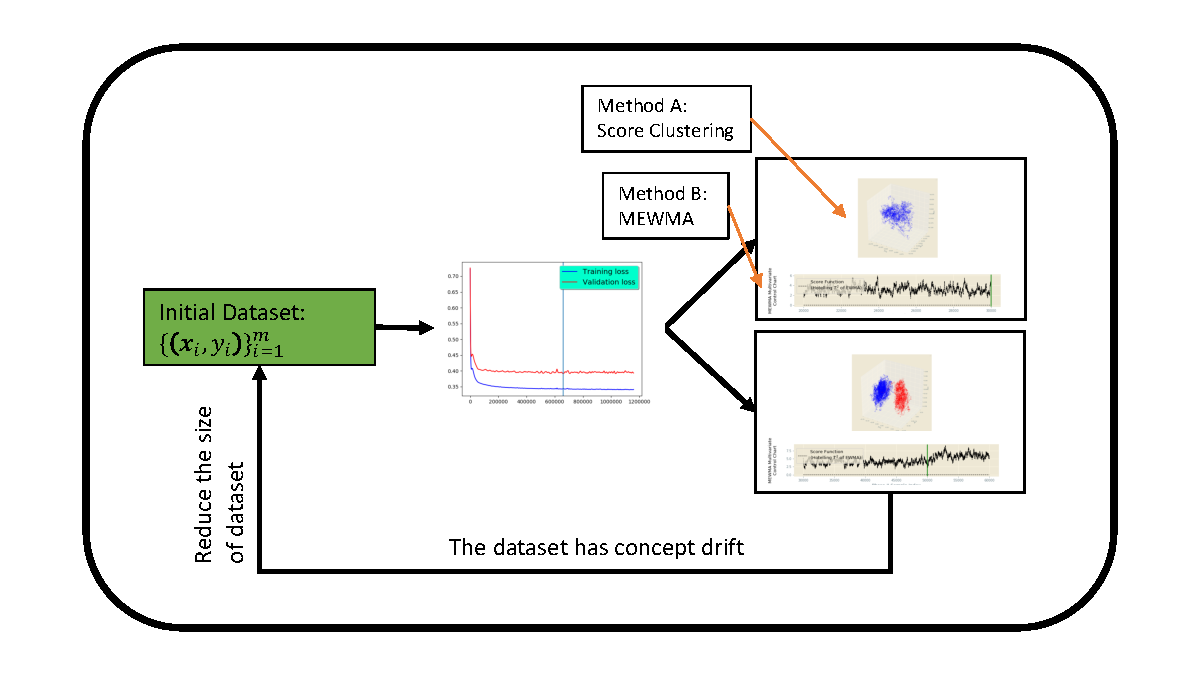
\includegraphics[width = 1\linewidth, trim=1.55in .85in 1.55in .85in, clip]{../figures/v14/flow_chart/Retrospective.png}
         \caption{Retrospective Analysis.}
         \label{fig:retro_analysis}
  \end{subfigure}
  \begin{subfigure}[t]{0.49\linewidth}
         \centering
         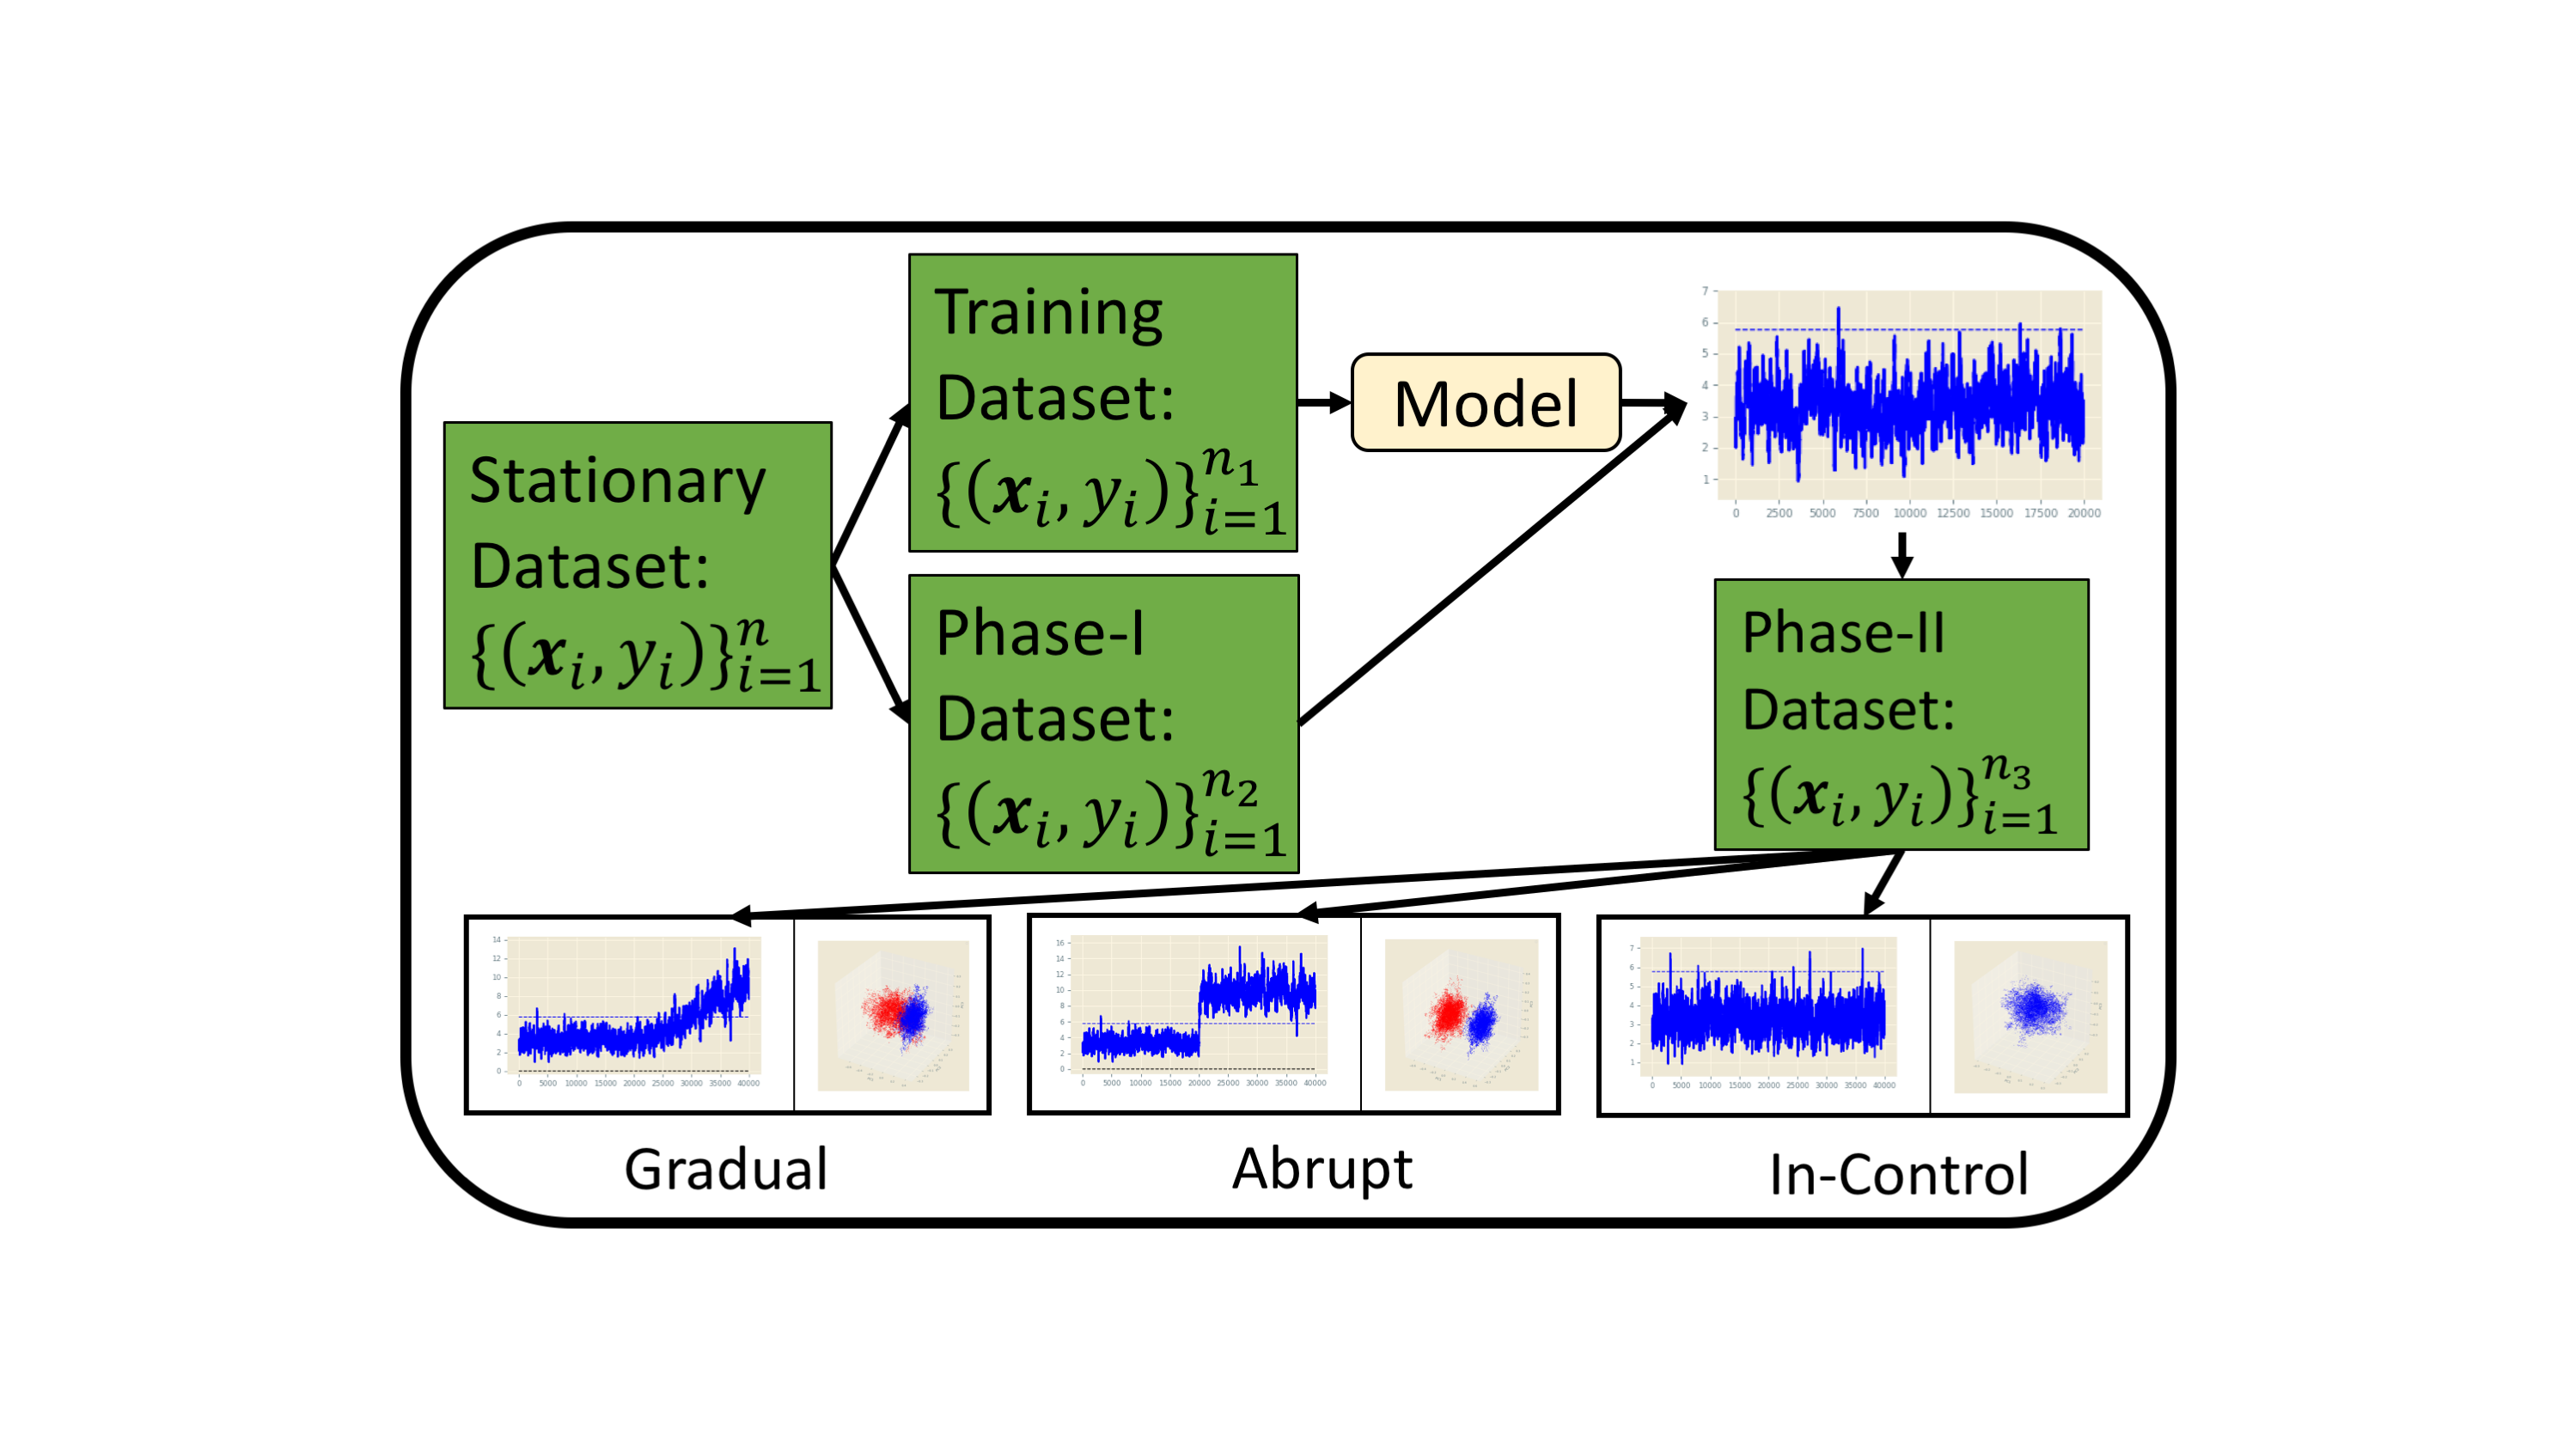
\includegraphics[width = 1\linewidth, trim=1.55in .85in 1.55in .85in, clip]{../figures/v14/flow_chart/Monitoring.png}
         \caption{Monitoring.}
         \label{fig:Monitoring}
  \end{subfigure}
  \begin{subfigure}[t]{0.49\linewidth}
         \centering
         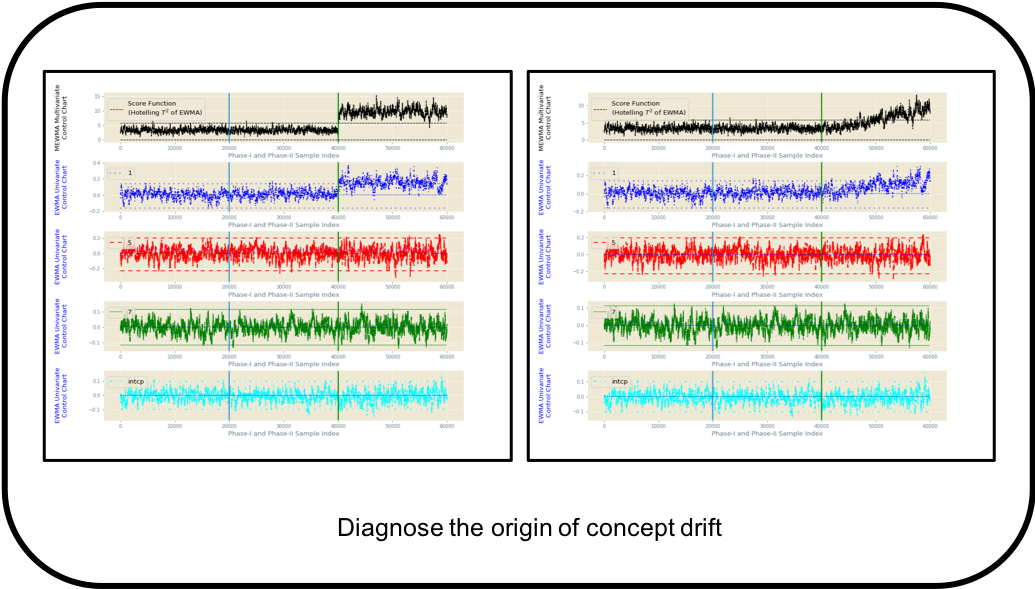
\includegraphics[width = 1\linewidth, trim=1.55in .85in 1.55in .85in, clip]{../figures/v14/flow_chart/Diagnose.png}
         \caption{Diagnosis.}
         \label{fig:diagnosis}
  \end{subfigure}
  \caption{ \replaced[id=Kungang, comment={}]{The framework of monitoring/detecting concept drift based on the score function. (a) Conducting retrospective analysis using MEWMA and/or score function clustering to ensure there is no concept drift in the dataset used to train and set control limits. The size of dataset can be recursively reduced if concept drift exists. (b) Monitoring concept drifts using the model and control limits obtained by processing training and Phase-I datasets. In this subplot, three examples of possible results are given: gradual and abrupt concept drift and in-control case. (c) Visualization of diagnosing concept drift: The MEWMA for score vectors and the EWMA for individual predictors are visualized to show the origin of concept drift.}{ The process of monitoring the score function using MEWMA. (a) Train a parametric model using batch or online learning method. (b) In Phase-I, make sure that the data are in-control and calculate control limits, as marked by the blue dashed-line. (c) In Phase-II, continue to monitor the new data for concept drift using the control limits calculated in Phase-I. The upper and lower figures show examples without and with concept drift.}}
  \label{fig:proc_mon_score}
\end{figure}

The score function is the first order derivative of the negative log-likelihood so that intuitively monitoring the score function is more sensitive than directly monitoring the negative log-likelihood. To demonstrate the efficacy of monitoring the score function, we compare it with other control charts monitoring EWMA of prediction error, or absolute residual, which are primarily used in the existing literatures. Classification error is defined as indicator function showing whether a prediction equals to true response ($I(\hat {y}_i \neq y_i)$); absolute residual is the absolute difference between real and predicted responses ($|\hat {y}_i - y_i|$). In later experimental studies, we show several advantages of the score function: monitoring the score function can render earlier detection of concept drift than monitoring those other statistics; monitoring components of the score function can help us diagnose which features contribute to the overall concept drift. Here, we show representative examples and analyses that concept drift results in mean change of score function but no change in classification error, which justifies the merit of using score-based method for concept drift problem. 

\subsubsection{Simple Logistic Regression}
\added[id=Kungang, comment={Comment: Even though the idea is intuitive, a clear explanation of the examples cannot be done in one or two sentences. Instead of over-complicating the motivation part, I just state the conclusion obtained from this example at the beginning and direct reader to this figure. I think that can also serve the purpose of motivation.}]{}
\begin{figure}[!htbp]
\centering
 \begin{subfigure}[t]{0.4\linewidth}
         \centering
         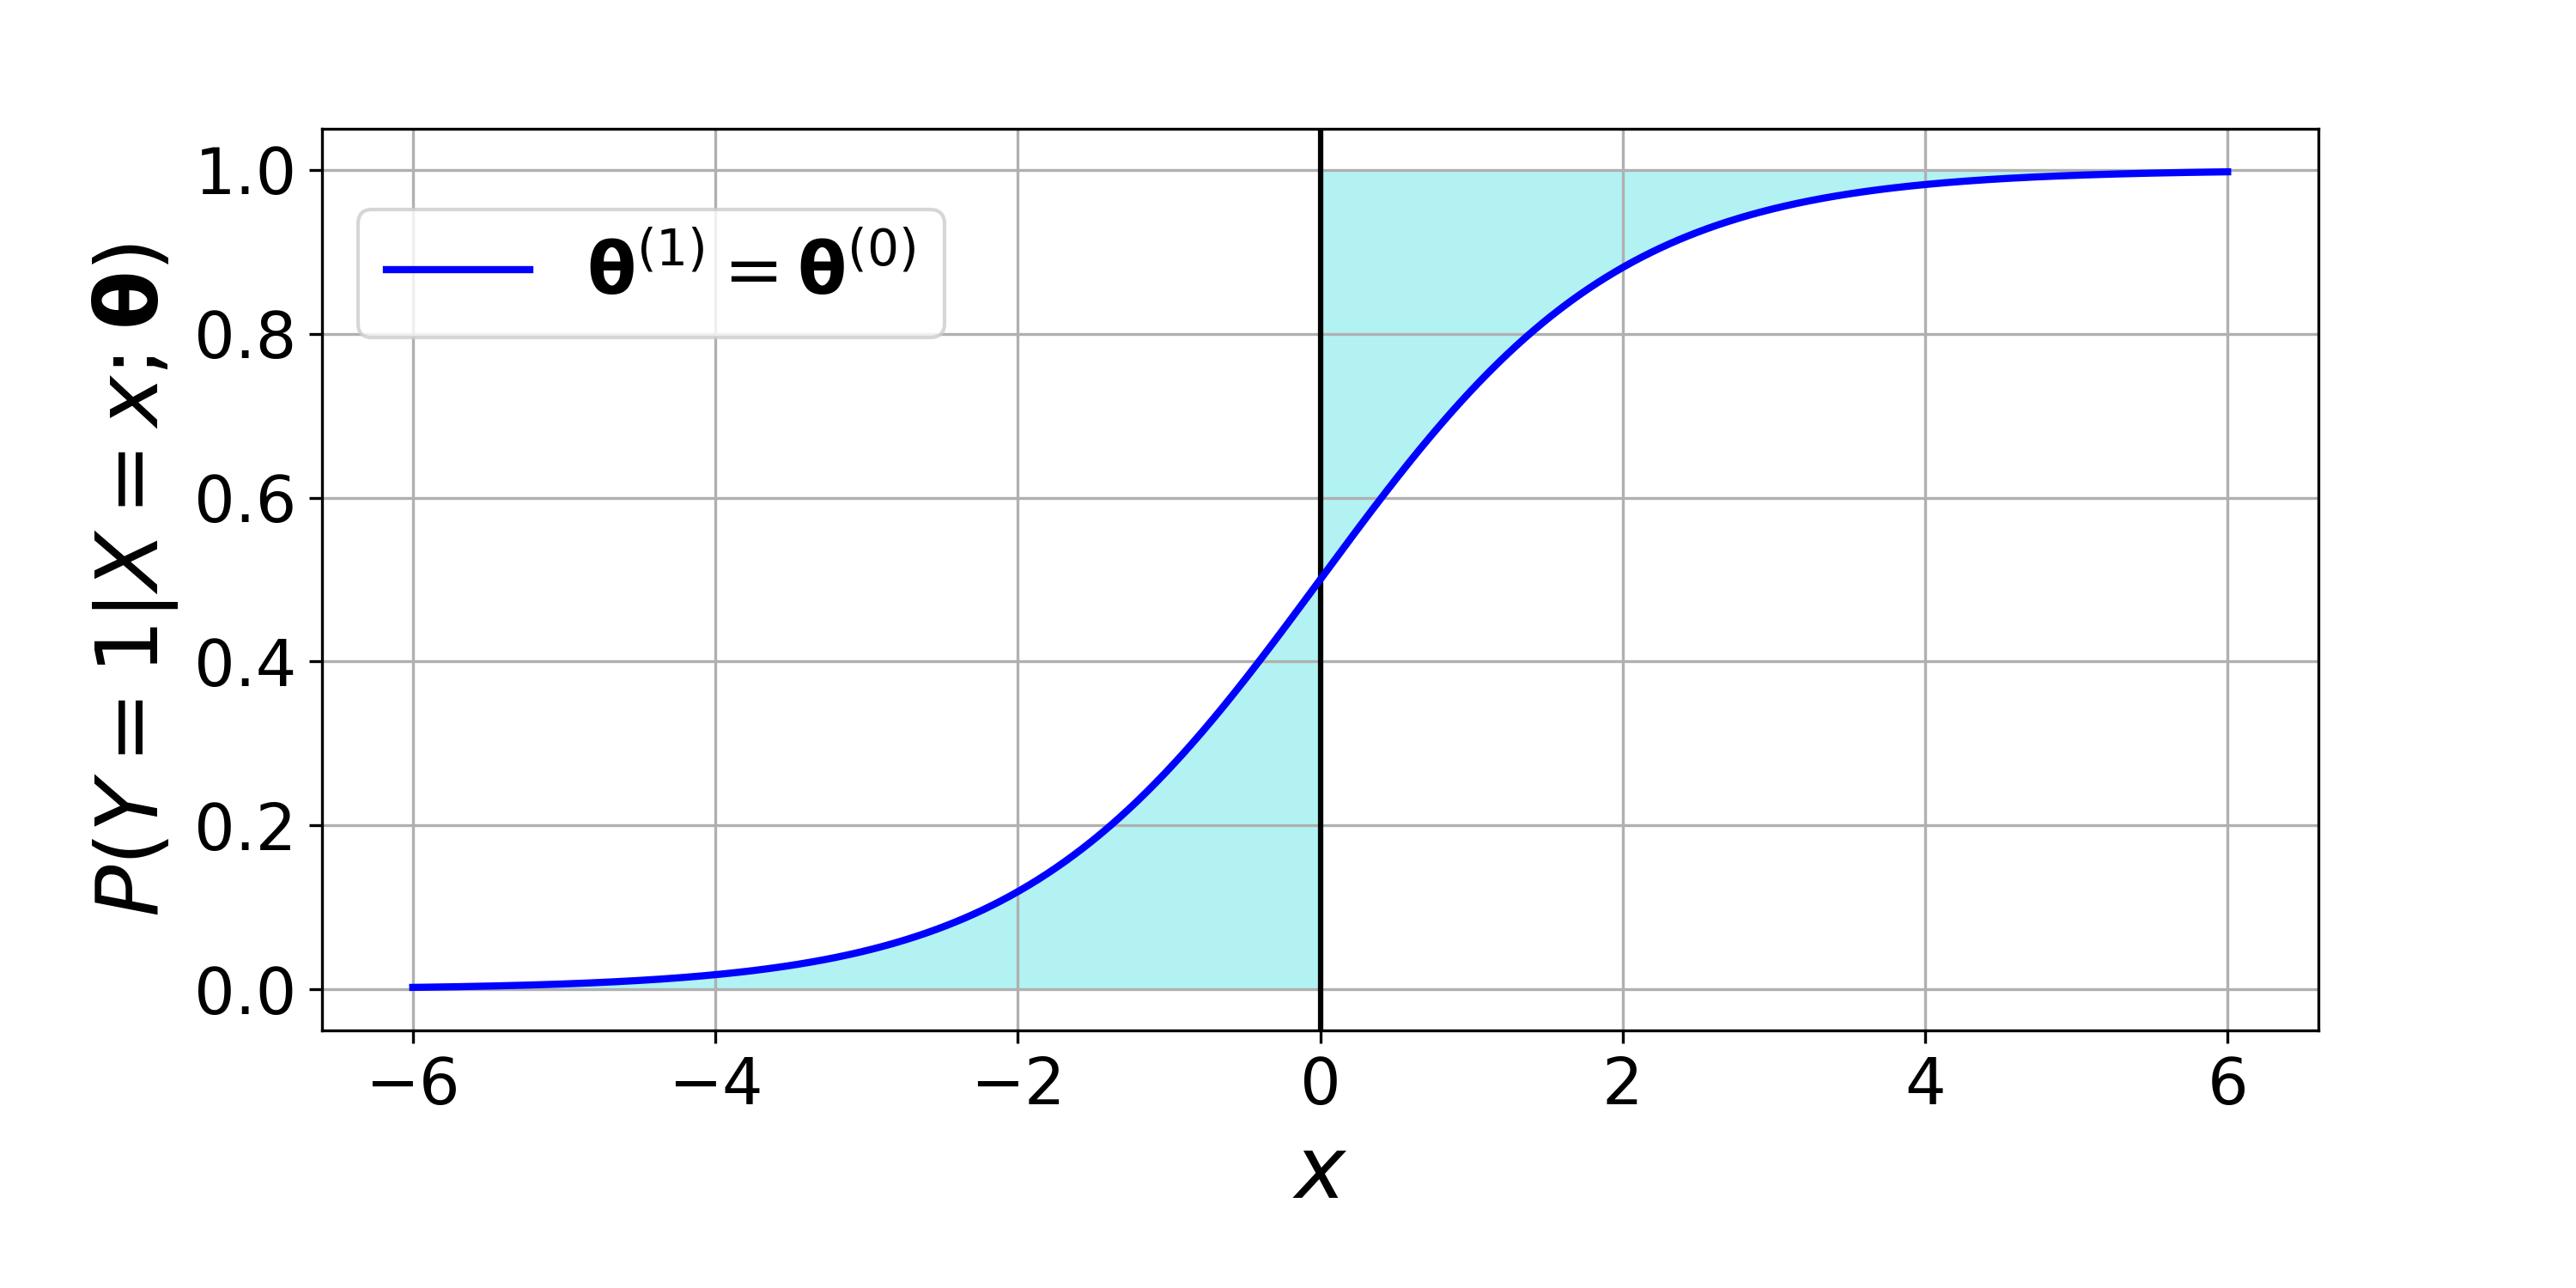
\includegraphics[width=\textwidth, trim=.2in .2in .7in .5in, clip]{../figures/v14/demons_fig/2D_logi_orig.png}
         \caption{The Original Data generating process and model.}
         \label{fig:logi_err_rate_unch_a}
  \end{subfigure}
  \begin{subfigure}[t]{0.4\linewidth}
         \centering
         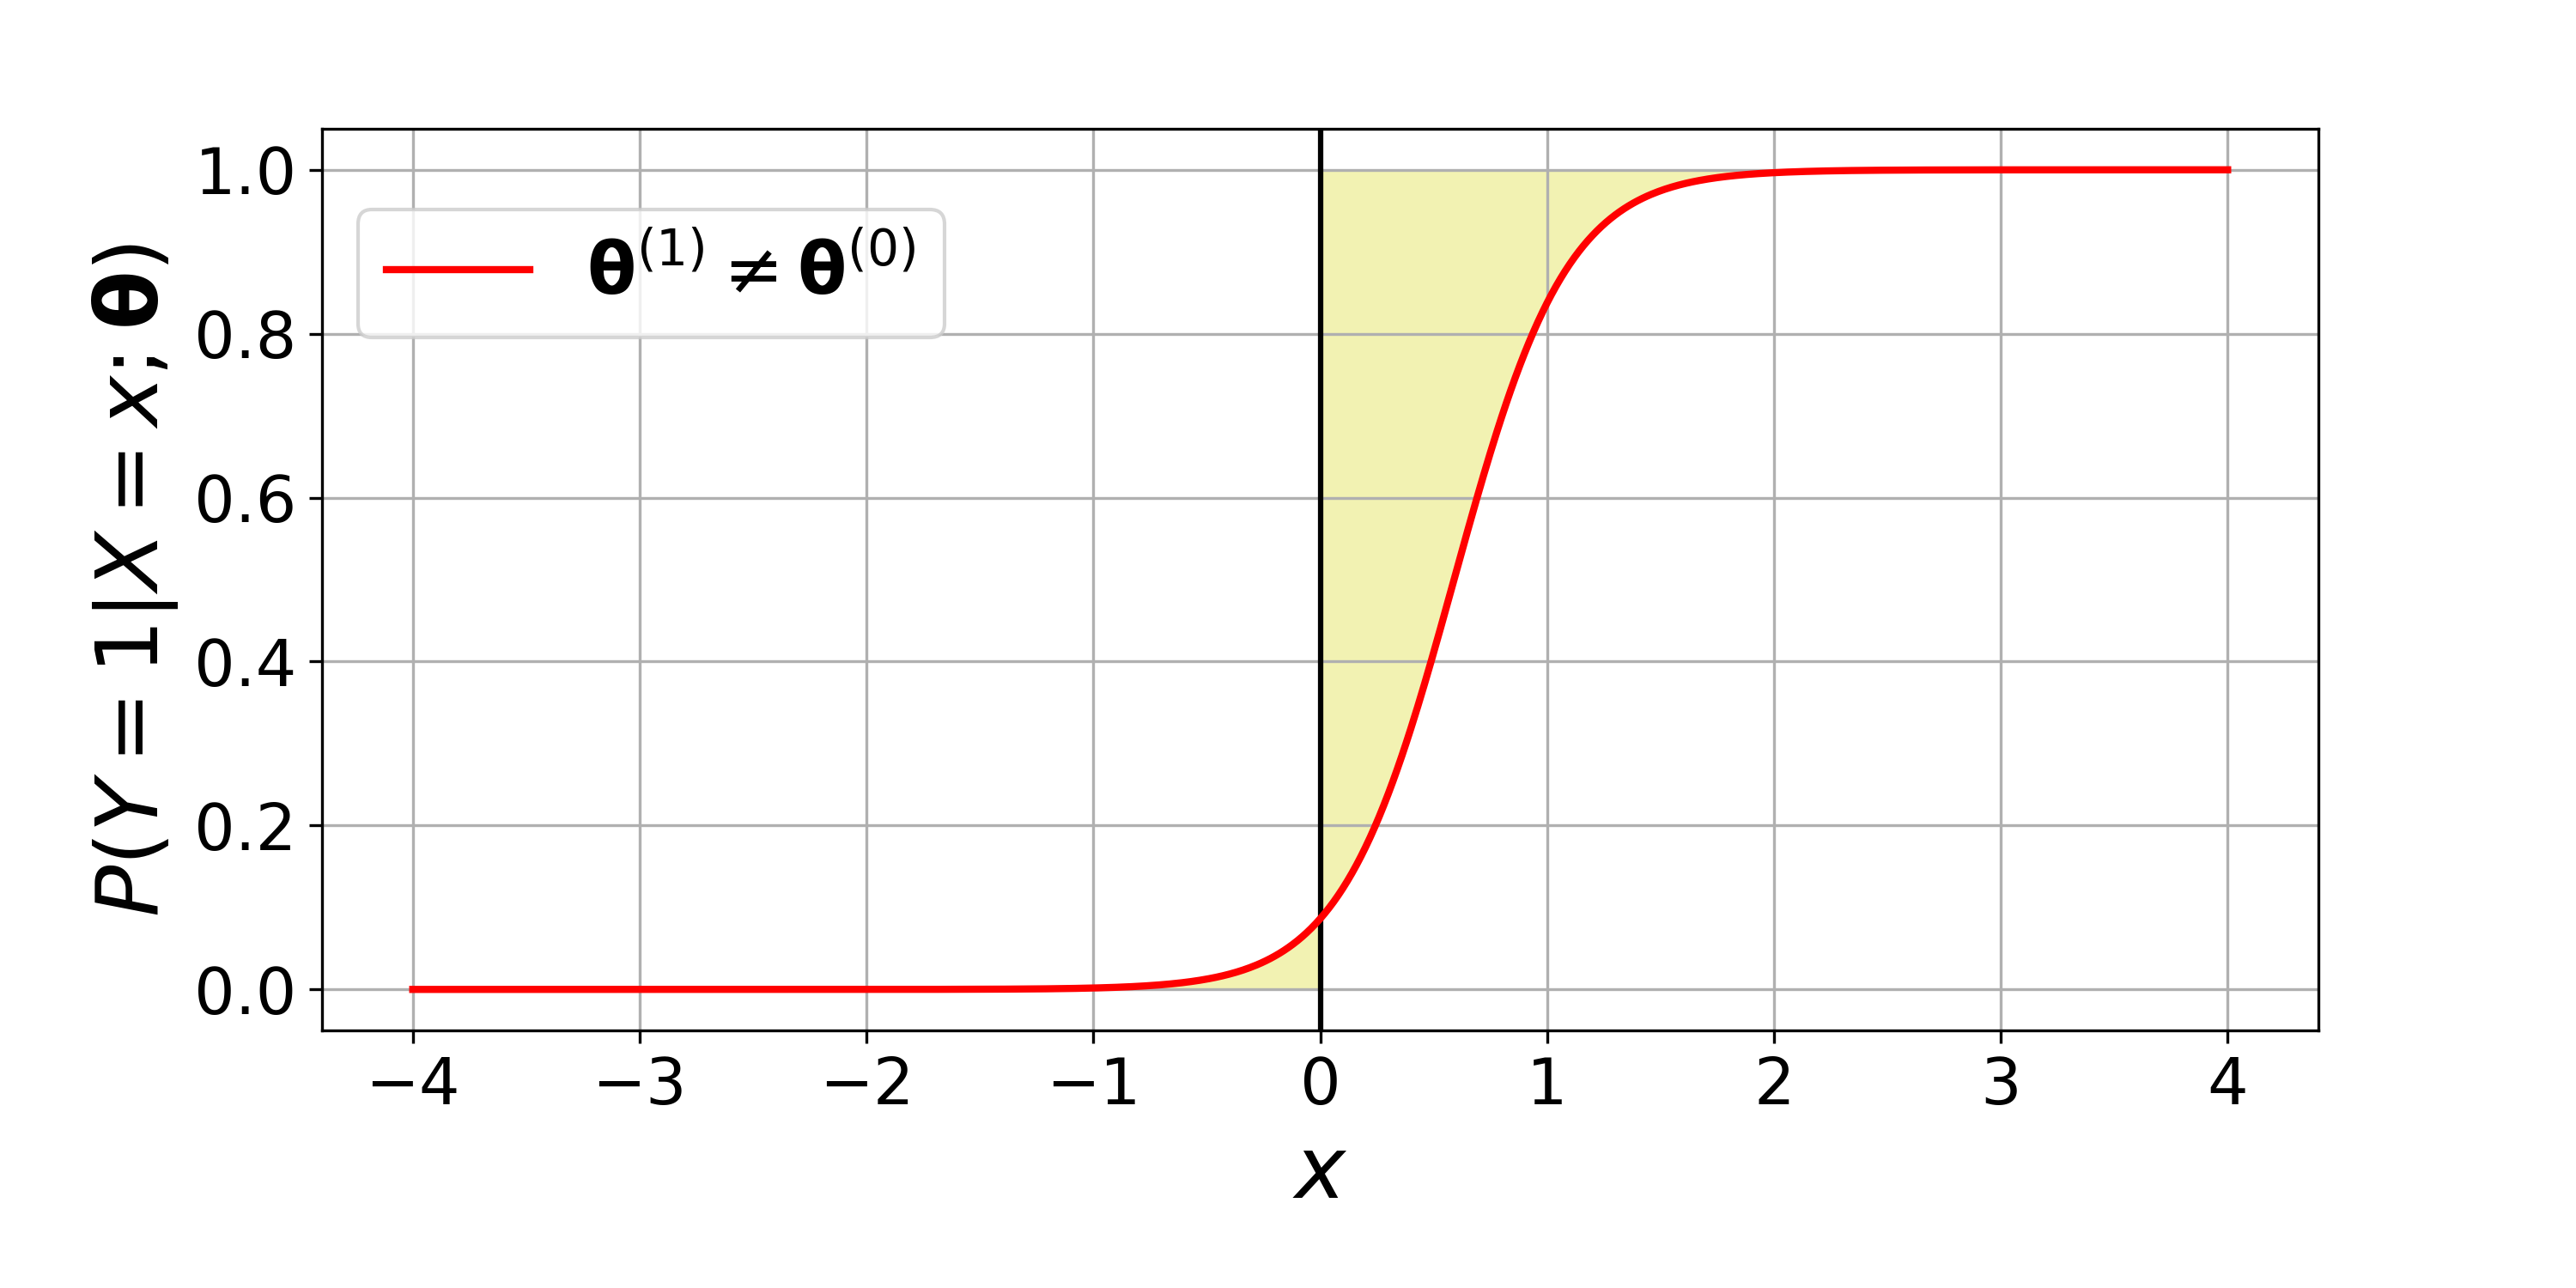
\includegraphics[width=\textwidth, trim=.2in .2in .7in .5in, clip]{../figures/v14/demons_fig/2D_logi_cd.png}
         \caption{The drifted data generating process.}
         \label{fig:logi_err_rate_unch_b}
  \end{subfigure}
%  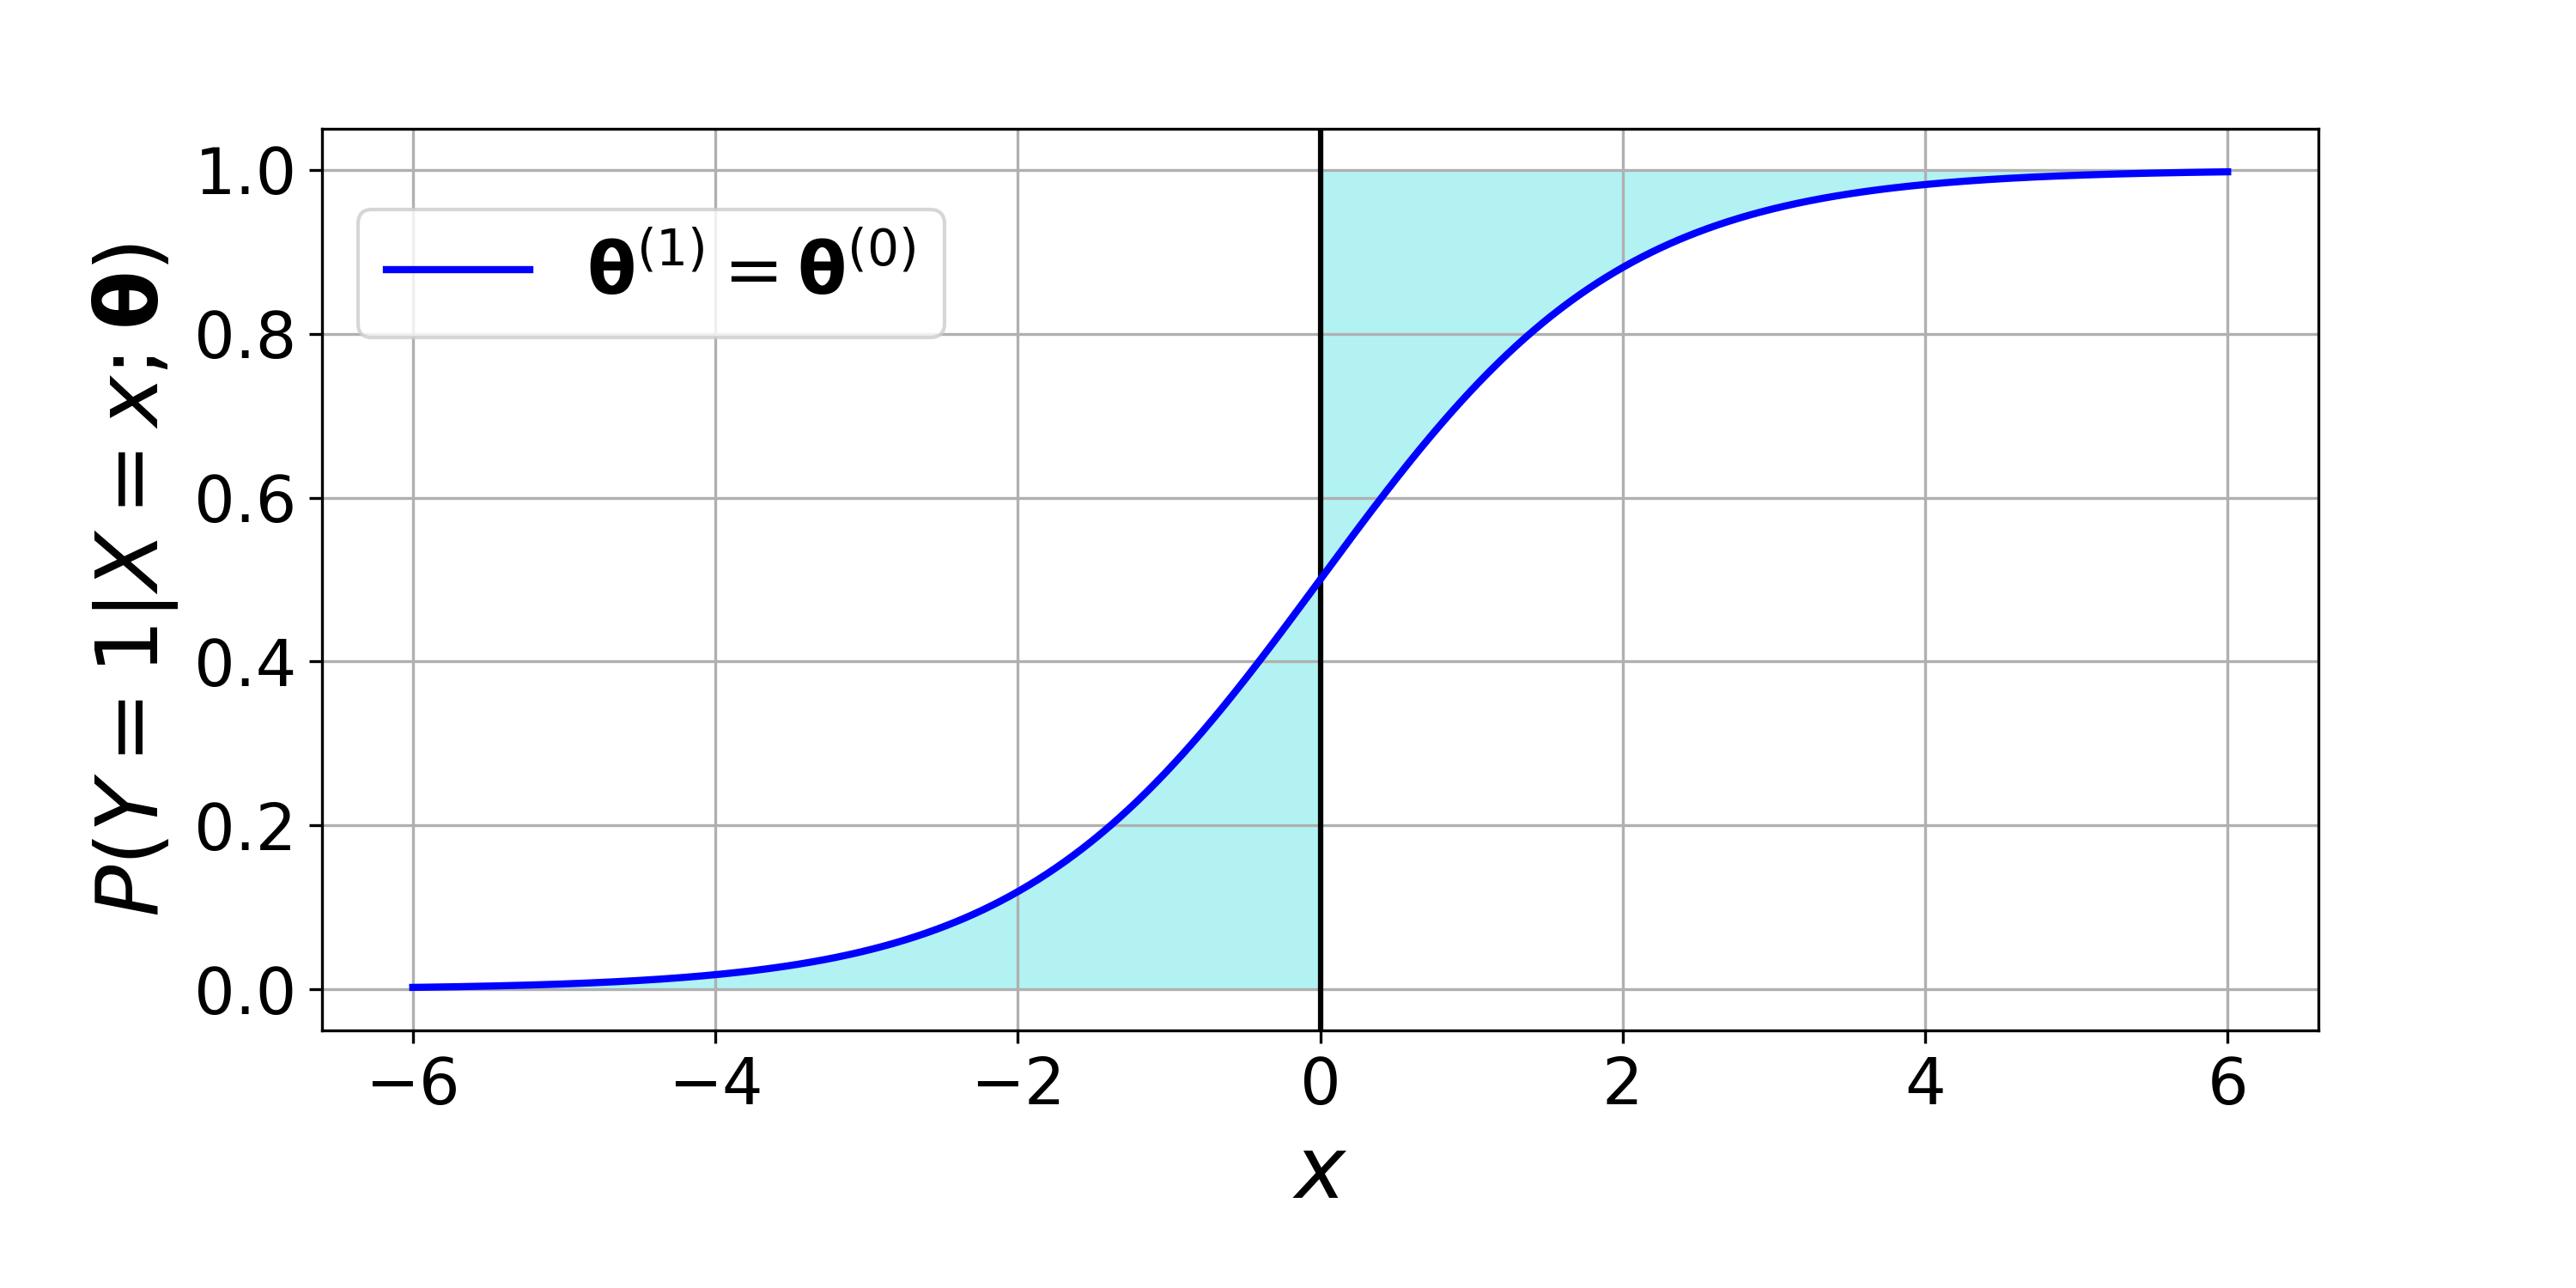
\includegraphics[width = 0.3\linewidth]{../figures/v14/demons_fig/2D_logi_orig.png}
%  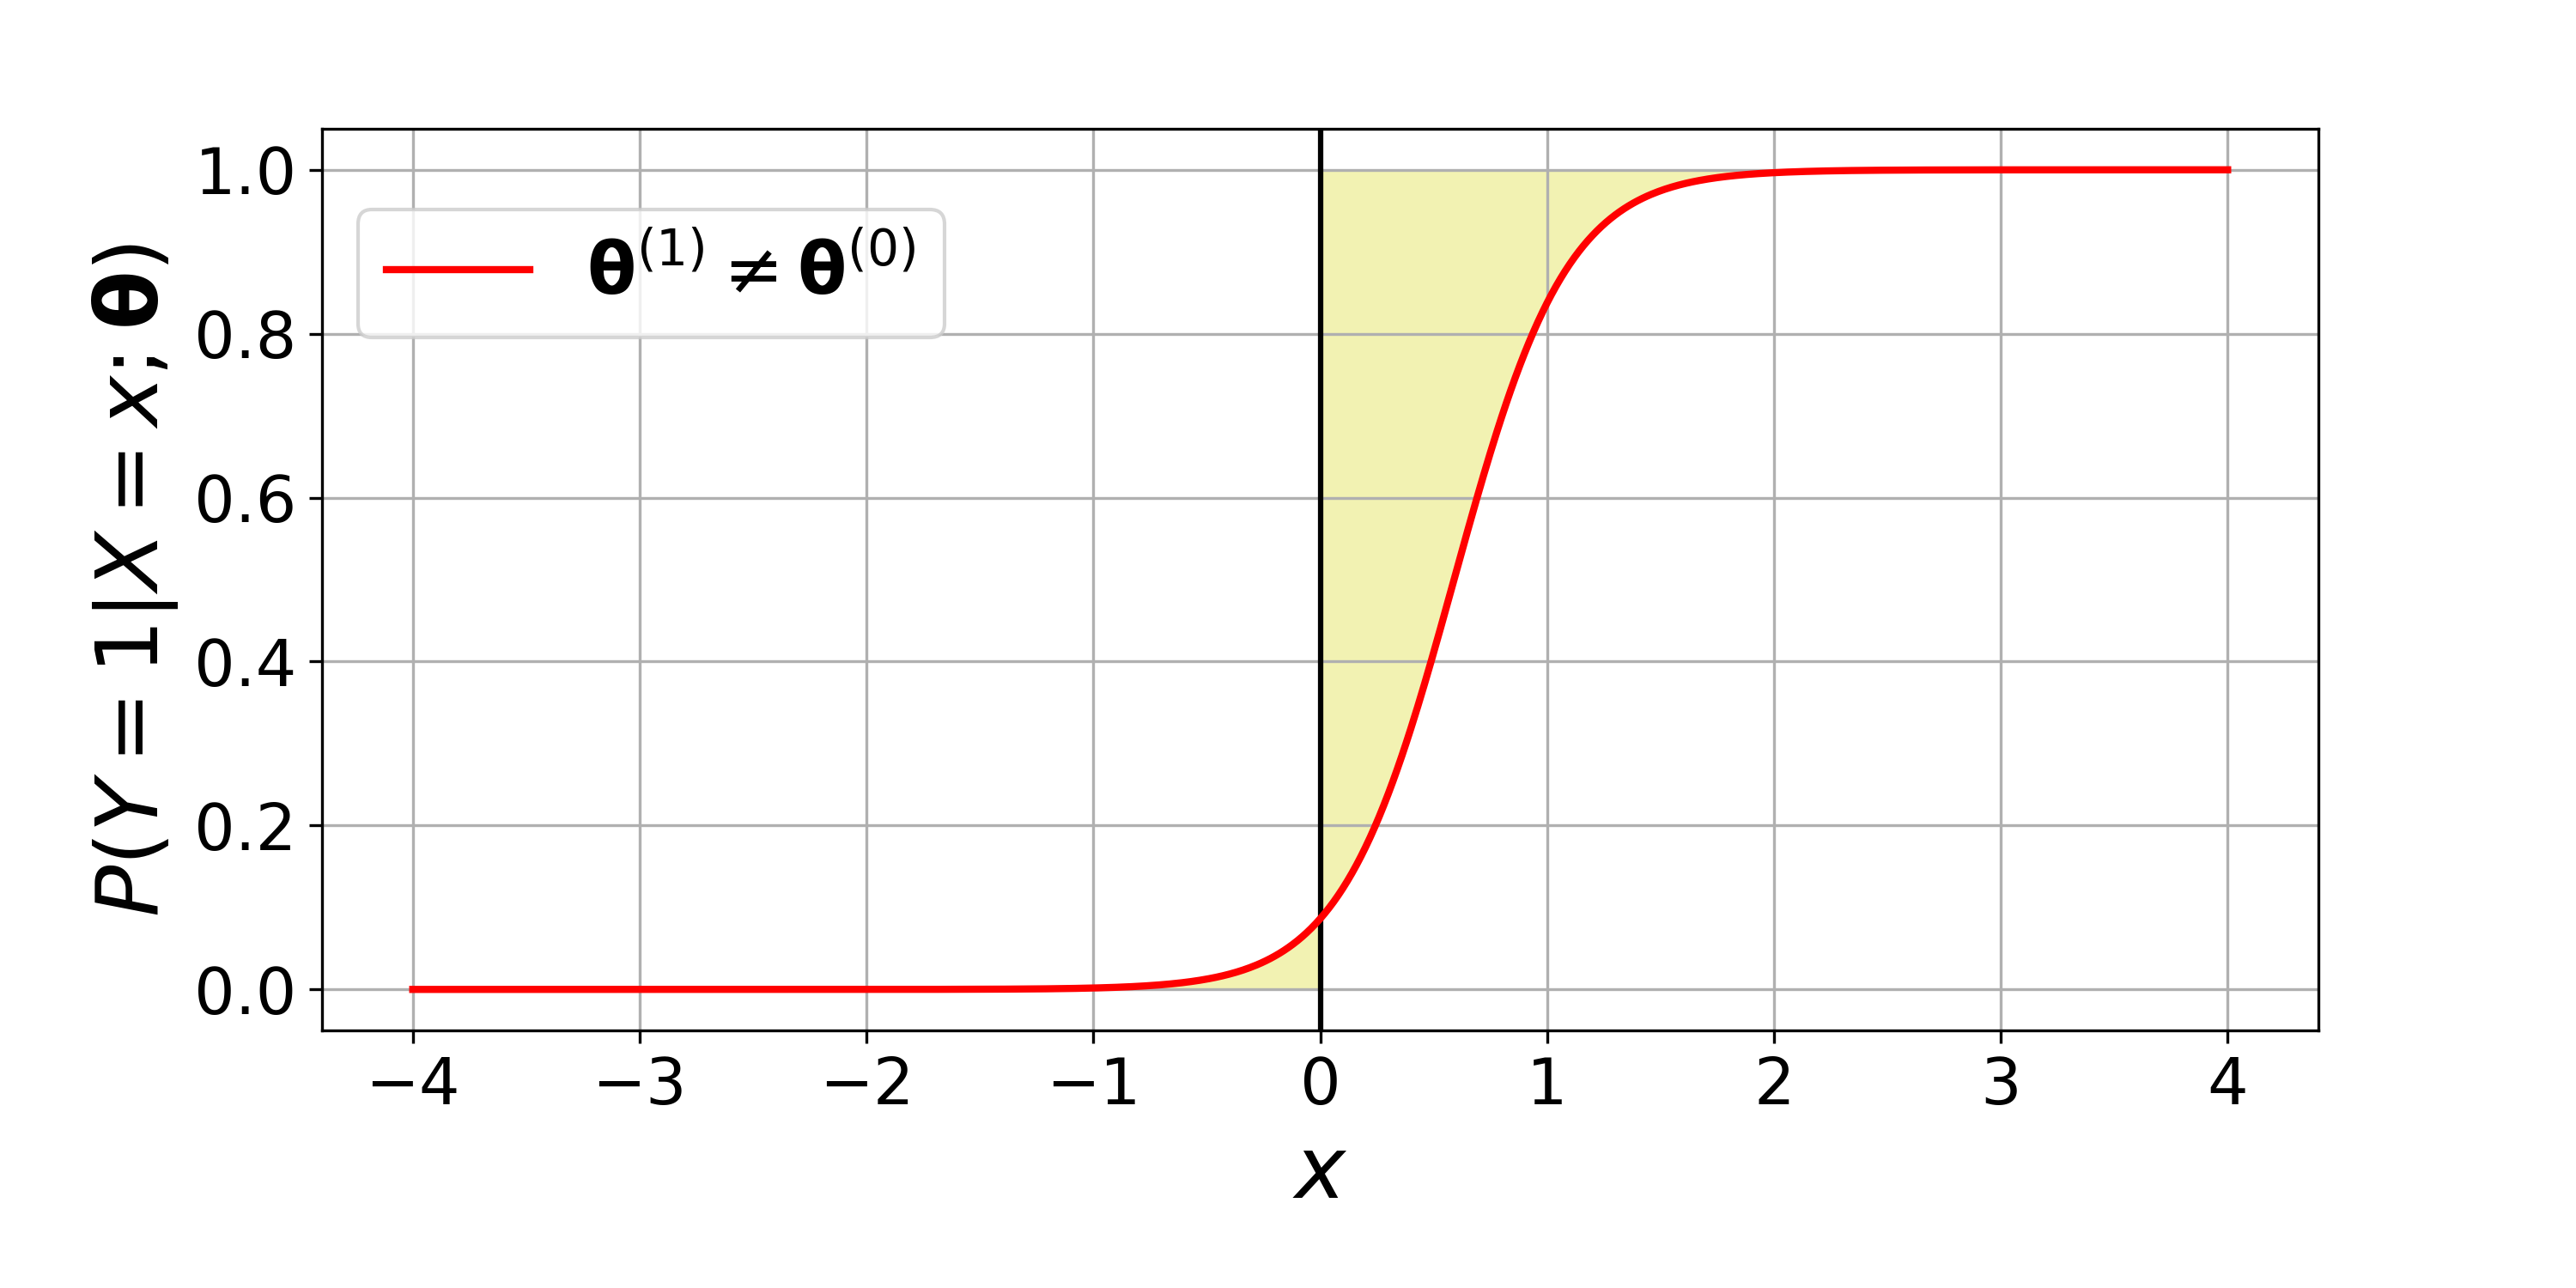
\includegraphics[width = 0.3\linewidth]{../figures/v14/demons_fig/2D_logi_cd.png}
 \begin{subfigure}[t]{0.6\linewidth}
         \centering
	 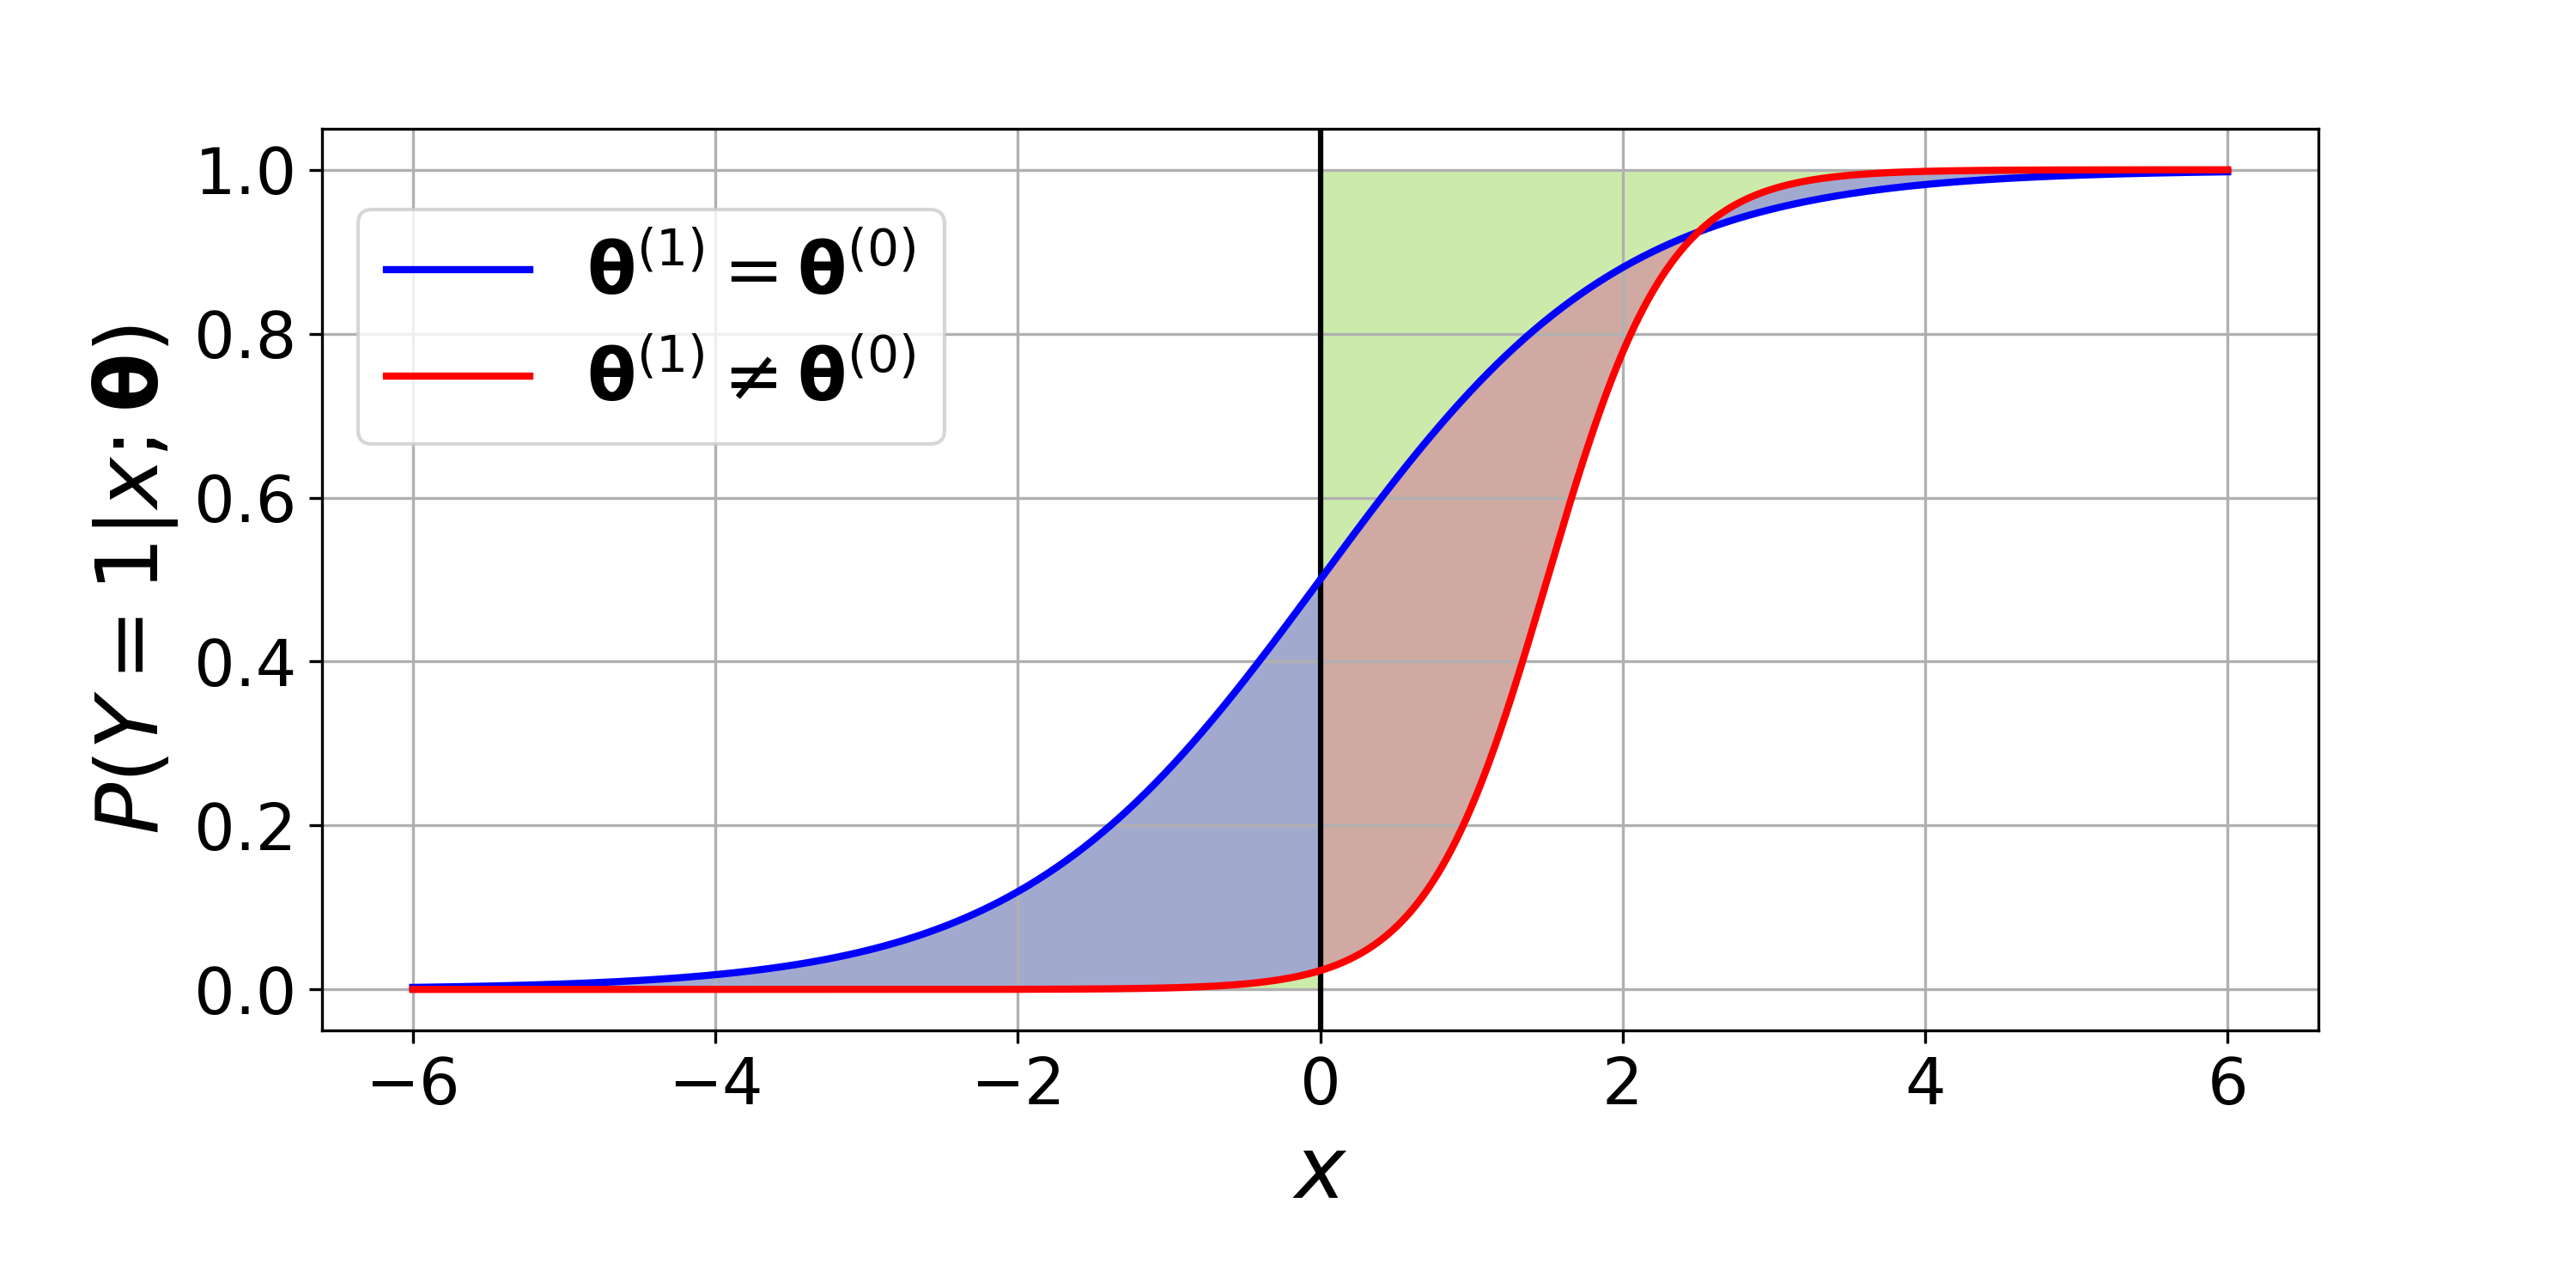
\includegraphics[width = \textwidth, trim=.2in .2in .7in .5in, clip]{../figures/v14/demons_fig/2D_logi.png}
         \caption{The overlap shaded area show unchanged expected error rate.}
         \label{fig:logi_err_rate_unch_c}
  \end{subfigure}
  \caption{The demonstration of simple logistic regression that concept drift would result in no change in expected error rate.}
  \label{fig:logi_err_rate_unch}
\end{figure}

For simple logistic regression, we can construct an example that concept drift happens without change in error rate. As shown in the Figure~\ref{fig:logi_err_rate_unch}, the blue solid line is the original model where binary data are generated according to Bernoulli distribution at each horizontal position $x$. We assume that the trained model almost perfectly captures the original model, so that the decision boundary is the $x=0$ (assuming we simplify the distribution of $x$ as uniform over $[-6, 6]$). After concept drift, the data generating model becomes the red line, where the optimal decision boundary has been changed. Error rate of the logistic regression model given predictor $\bm {X}$ can be written as a penalty function:
\begin{align}
C _{err}(\bm {X}) = p ^{(1)}I(\hat{y}=0)+(1-p ^{(1)})I(\hat{y}=1)
\label{eqn:penal_err}
\end{align}
where $p ^{(1)} = P(Y=1|\bm {X}, \bm { \theta} ^{(1)})$ and the superscript indicates that this is the probability function after a decision model being trained. Thus, if concept drift happens after training, $p ^{(1)} \neq p ^{(0)}$; otherwise, they are equal. Notice that the probability function $p ^{(1)}$ depends on predictor vector $\bm {X}$, but it would be omitted for clean notation. Given the distribution of covariates $\bm {X}$ and decision rule (model) $\hat{y}$, the expectation of this penalty function are those shaded areas in the Figure~\ref{fig:logi_err_rate_unch_a} and \ref{fig:logi_err_rate_unch_b} for the original (blue) and the drifted (yellow) data generating process. In the Figure~\ref{fig:logi_err_rate_unch_c}, the drifted data generating process decreases the error by those blue shaded error but adds the red shaded area as new error. Because the two areas are equal, the expected error rate remains the same. If we only monitor the error rate or any metrics derived from it, the concept drift would be missed. More important, this concept drift changes the optimal decision boundary, so that retraining the model can potentially obtain higher accuracy. 

\begin{figure}[!htbp]
\centering
 \begin{subfigure}[t]{0.49\linewidth}
         \centering
         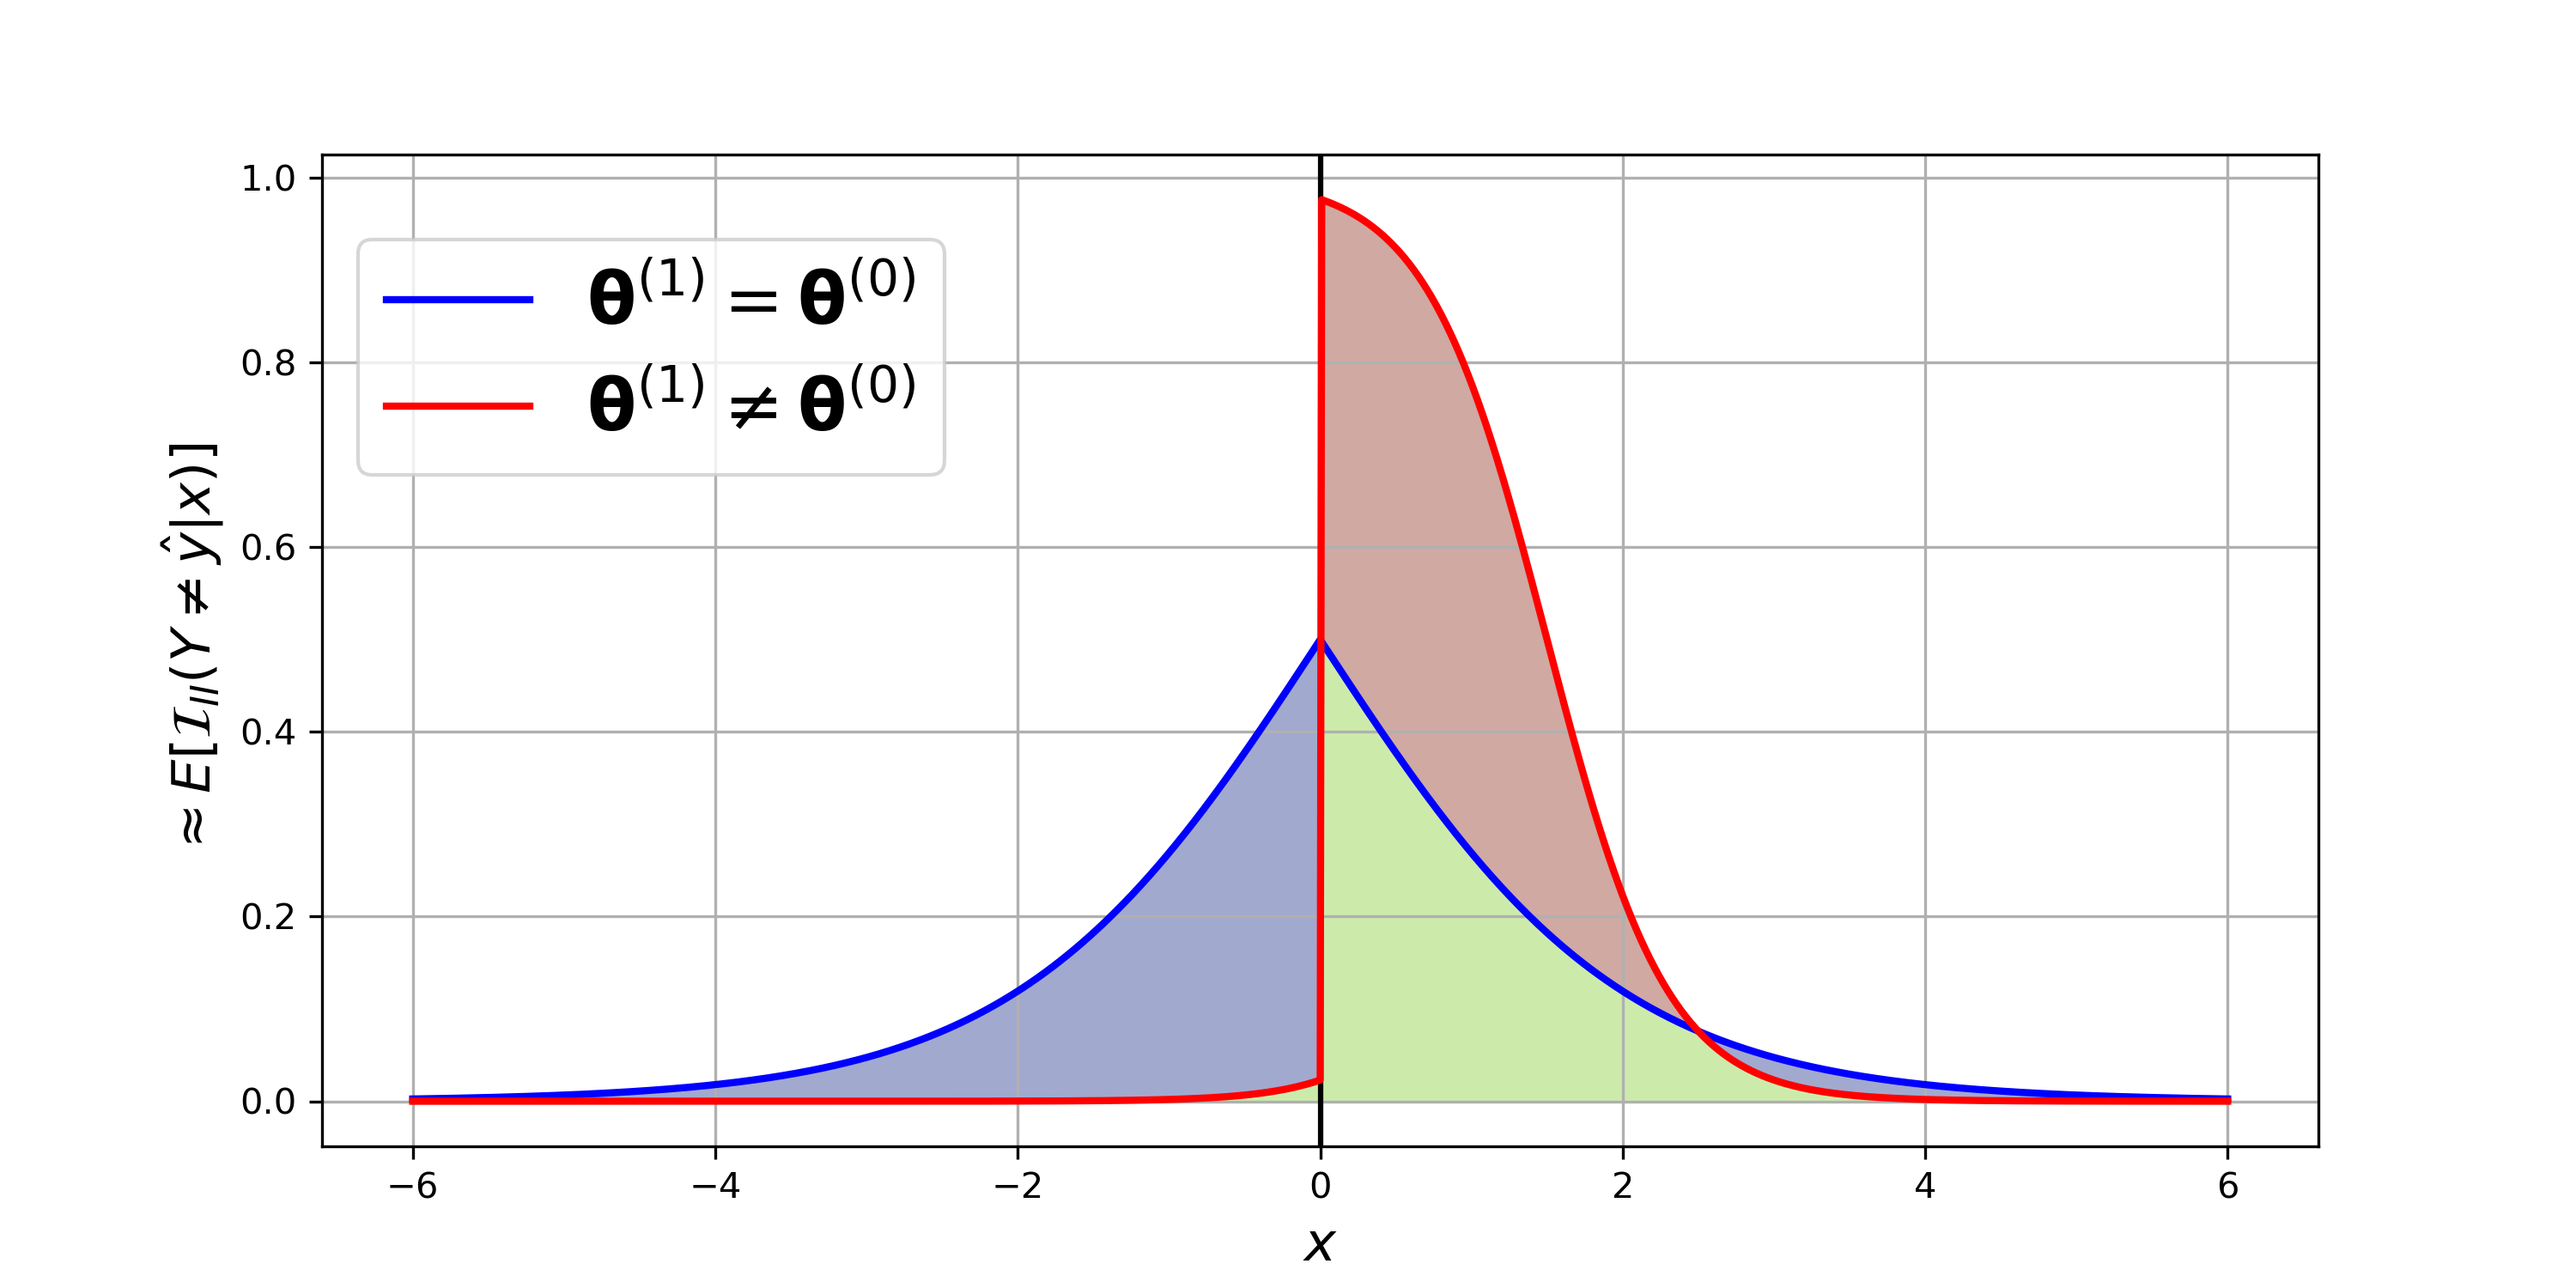
\includegraphics[width=\textwidth, trim=.2in .2in .7in .5in, clip]{../figures/v14/demons_fig/2D_err_logi.png}
         \caption{The penalty function before and after concept drift by monitoring error.}
         \label{fig:logi_err_rate_penal}
  \end{subfigure}
%  \begin{subfigure}[t]{0.32\linewidth}
%         \centering
%         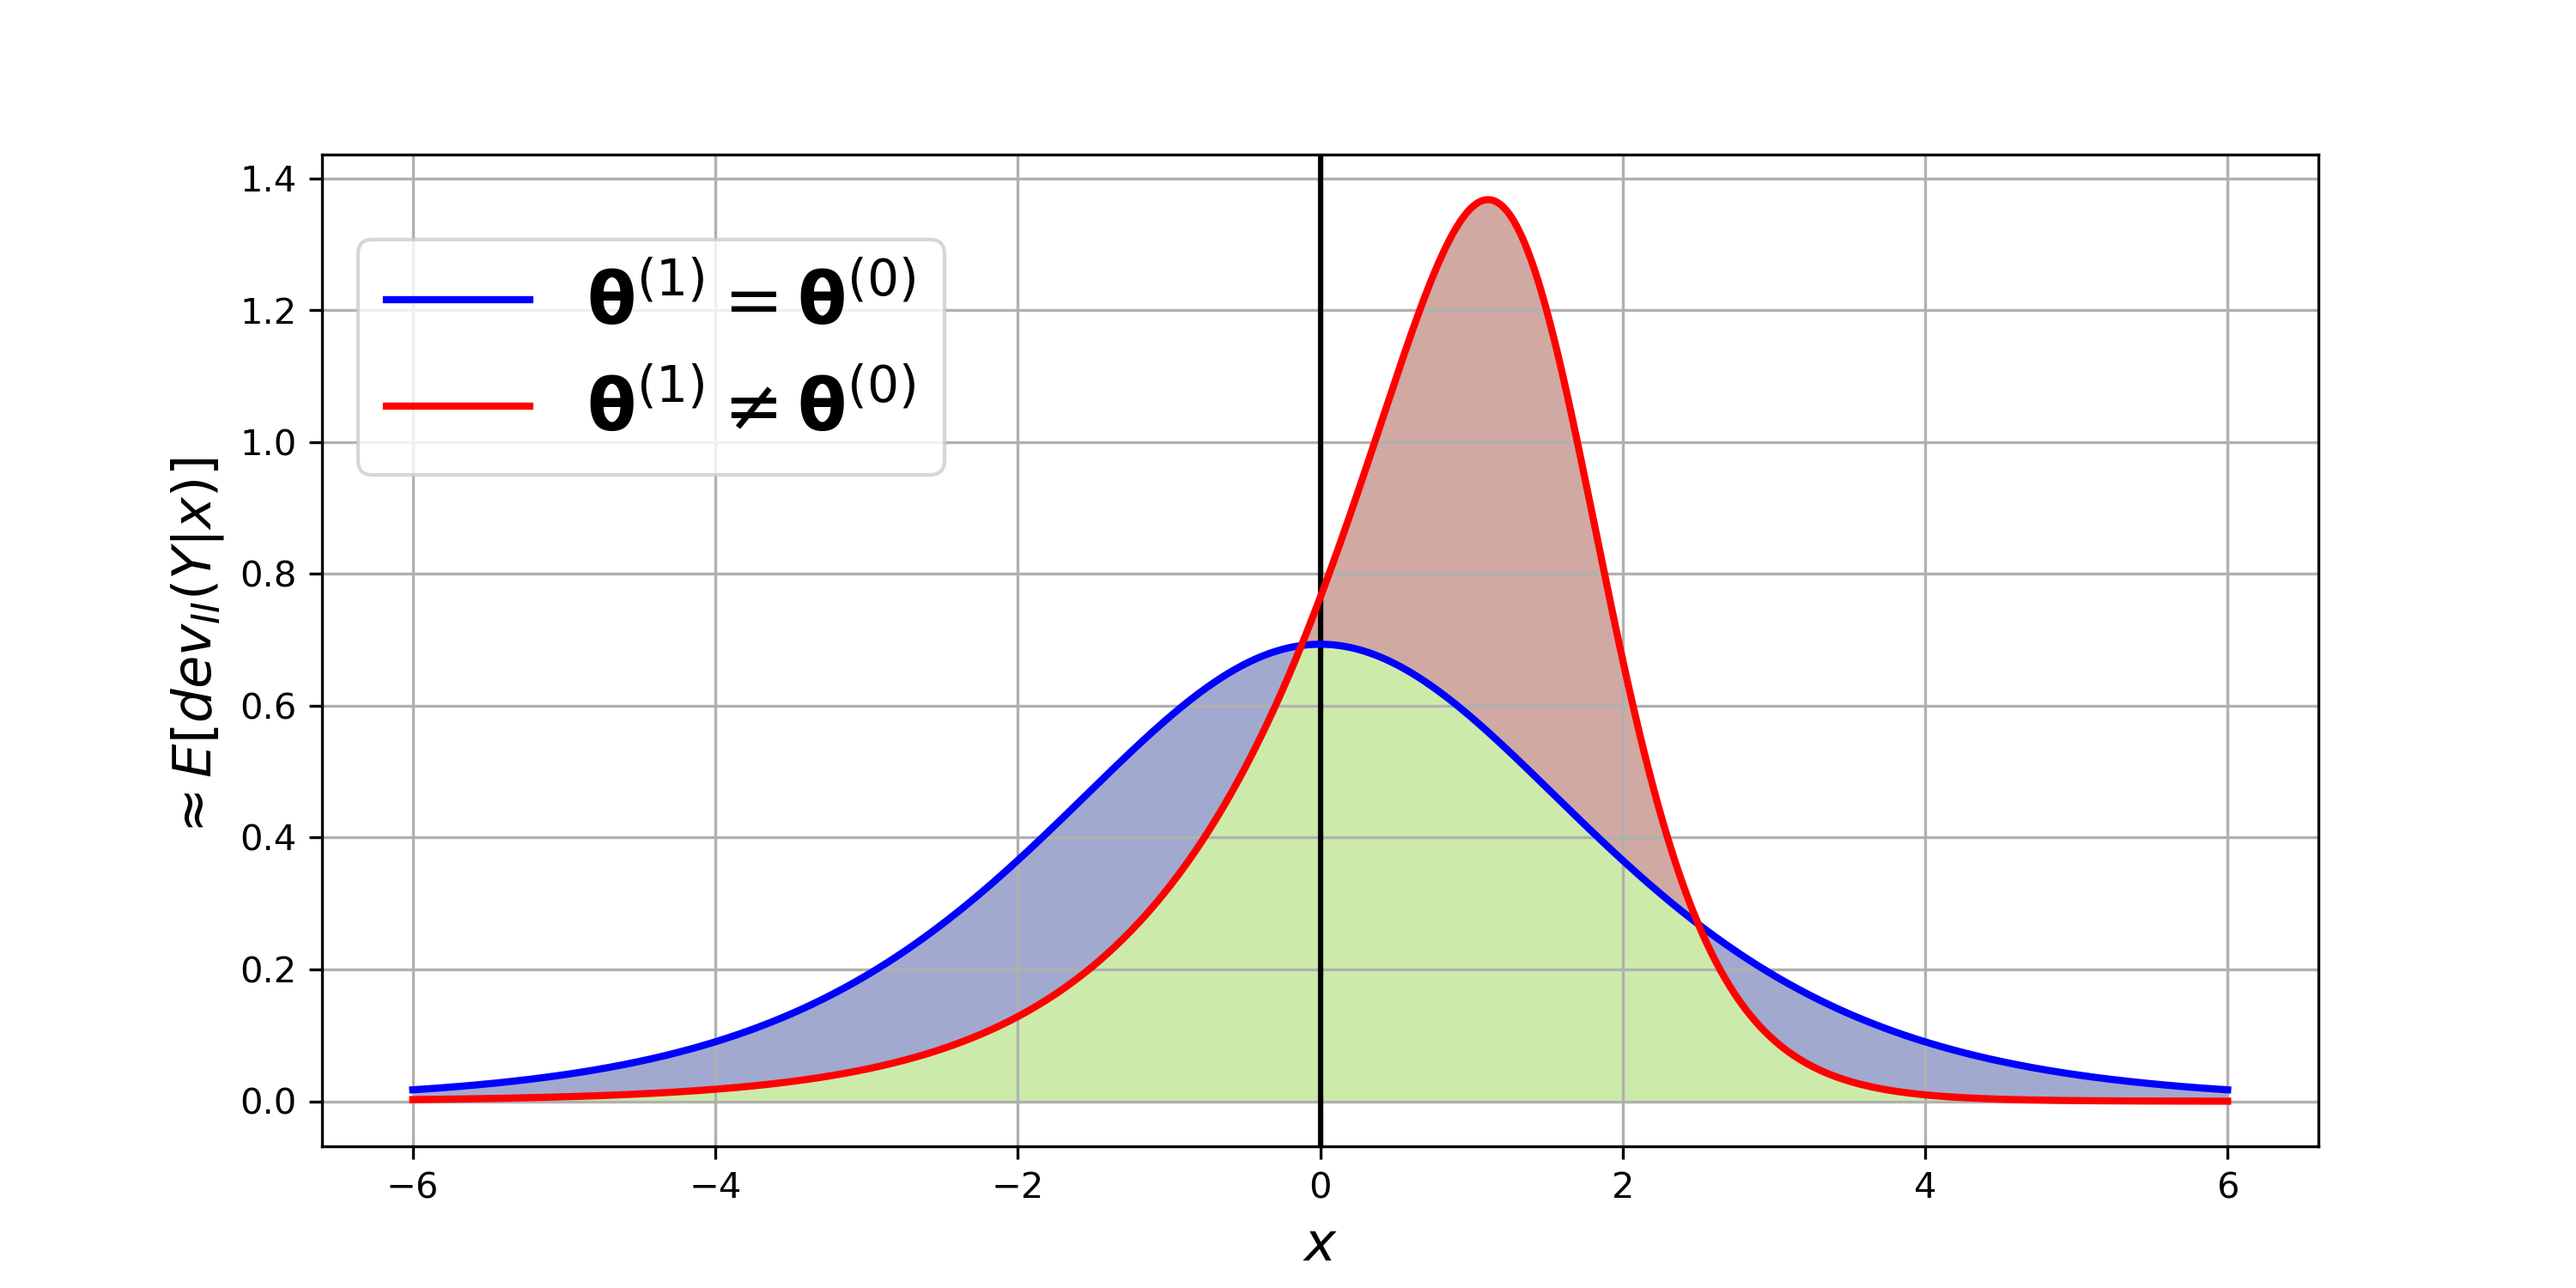
\includegraphics[width=\textwidth]{../figures/v14/demons_fig/2D_dev_logi.png}
%         \caption{The penalty function before and after concept drift by monitoring deviance.}
%         \label{fig:logi_dev_rate_penal}
%  \end{subfigure}
 \begin{subfigure}[t]{0.49\linewidth}
         \centering
	 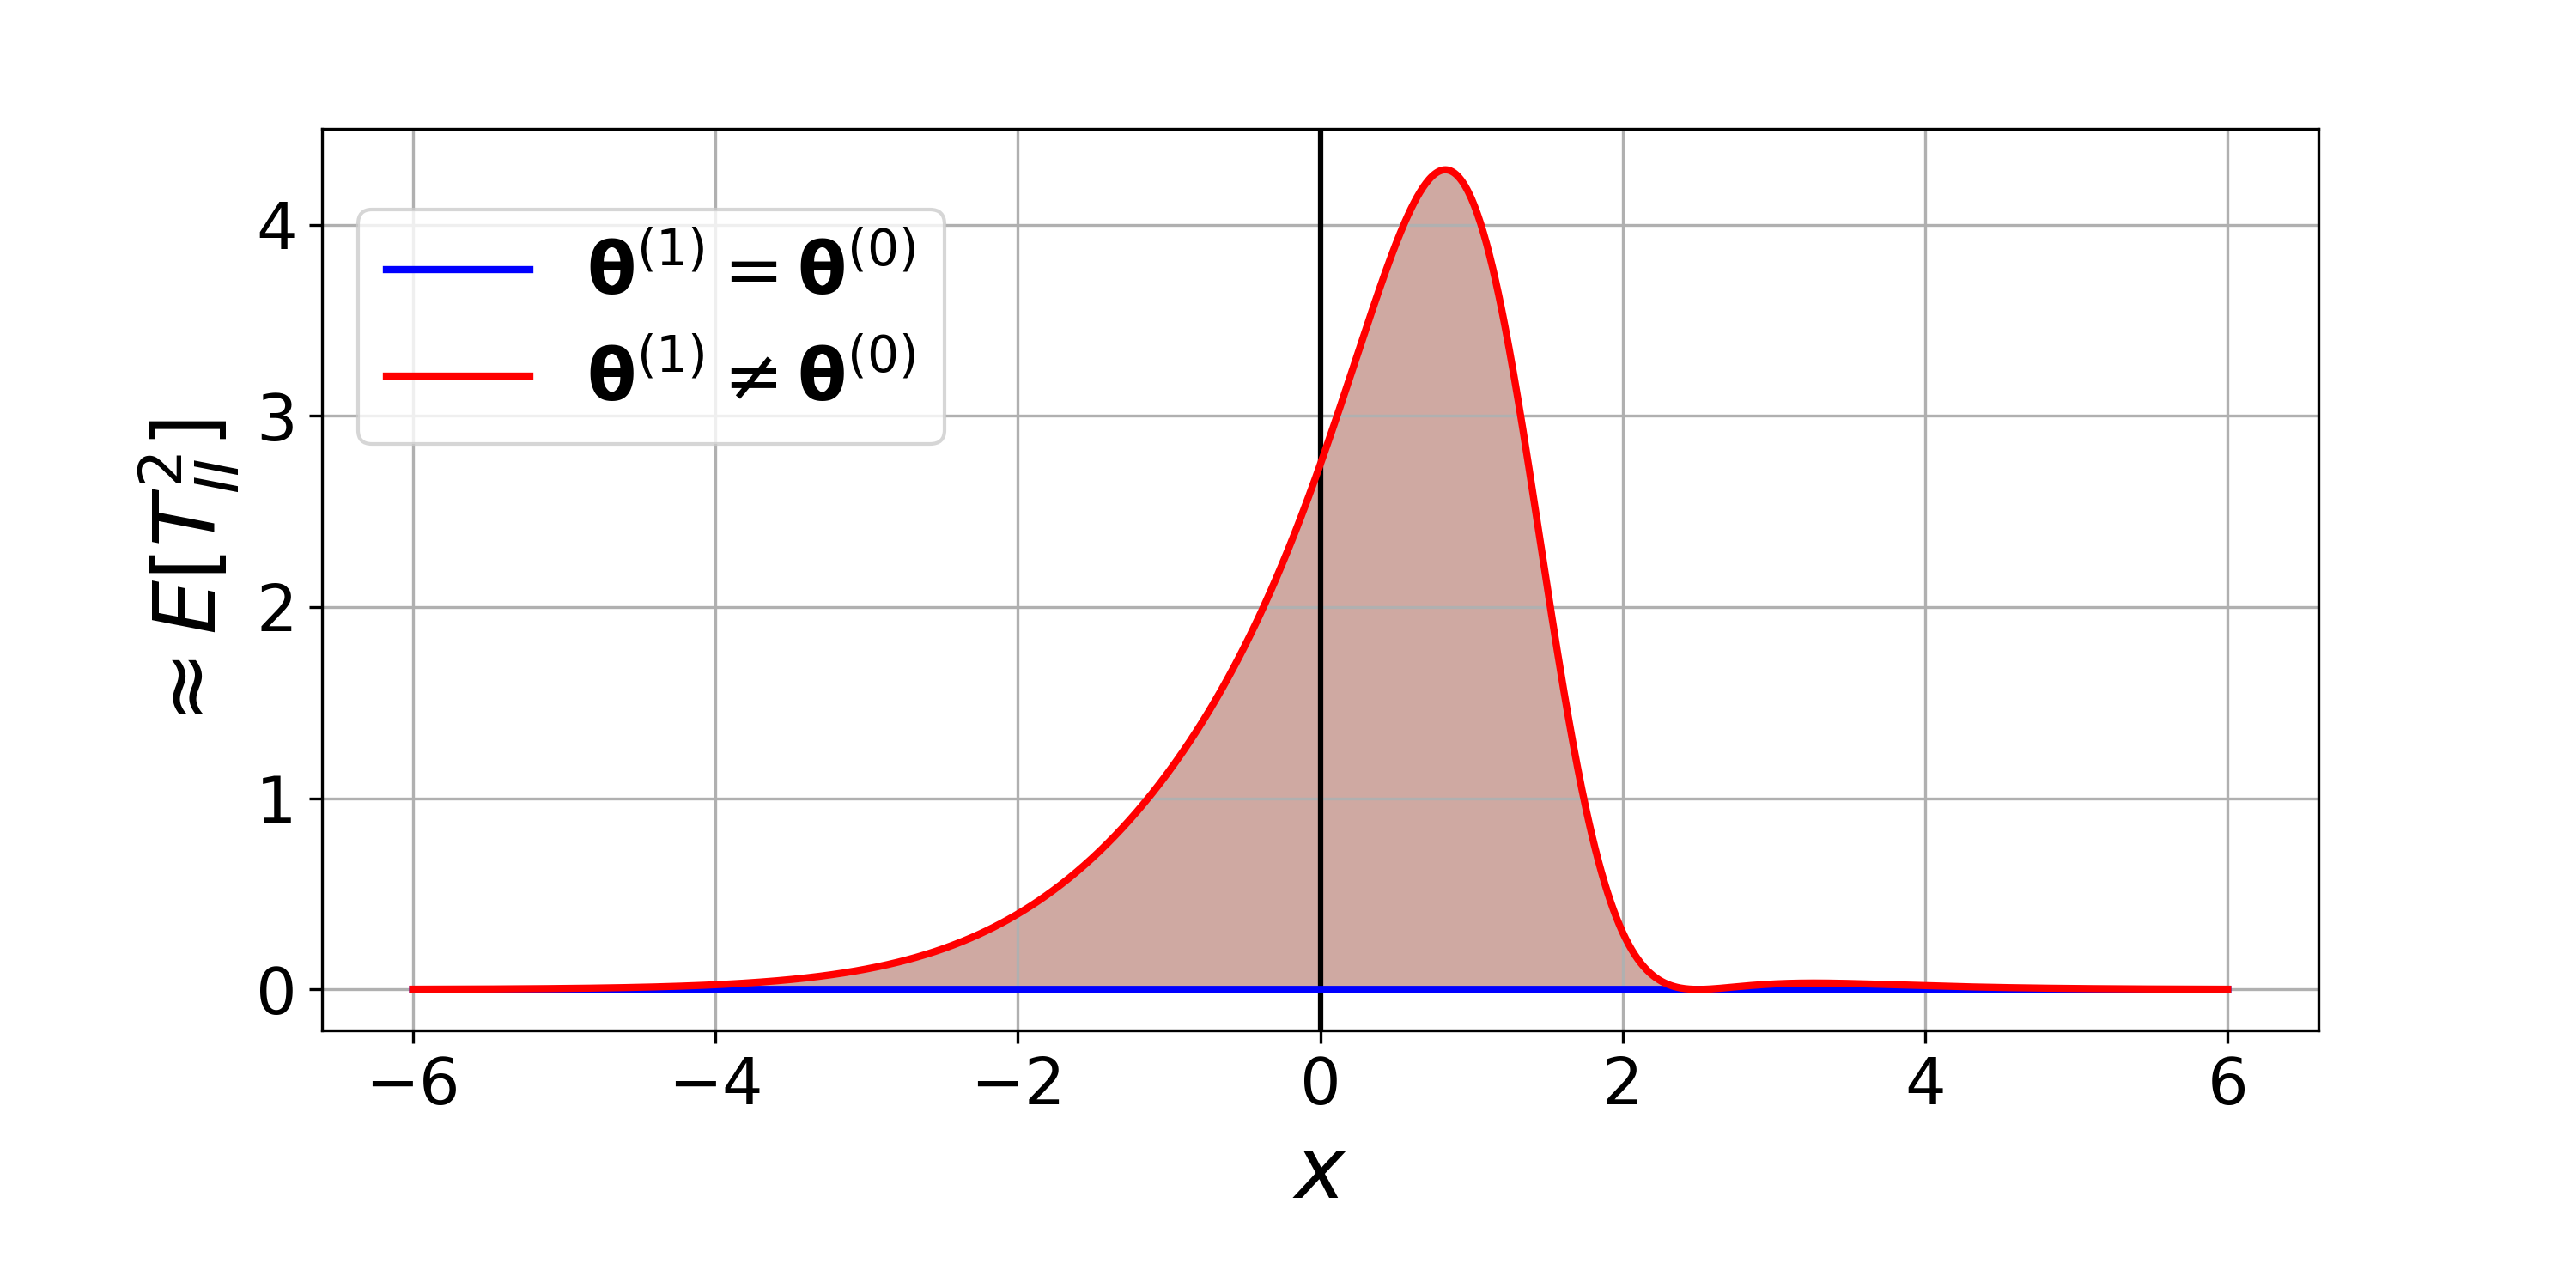
\includegraphics[width = \textwidth, trim=.2in .2in .7in .5in, clip]{../figures/v14/demons_fig/2D_score_logi.png}
         \caption{The penalty function before and after concept drift by monitoring Hotelling $T^2$ of the score function.}
         \label{fig:logi_score_rate_penal}
  \end{subfigure}
  \caption{The comparison of penalty functions by monitoring classification error and Hotelling $T^2$ of EWMA of the score function.}
  \label{fig:logi_med_penal}
\end{figure}

This can be generalized into other penalty functions for metrics like Hotelling $T^2$ of EWMA of the score function as mentioned in the Section~\ref{ss:MEWMA}. For ease of eyes, penalties are put close to horizontal line $y=0$, so that the expectation of monitored penalty equals the area under the curve in the Figure~\ref{fig:logi_med_penal}. 
%The penalty function for deviance is:
%\begin{align}
%C _{dev}(\bm {X})=-p ^{(1)}\log p ^{(0)}-(1-p ^{(1)})\log(1-p ^{(0)})
%\label{eqn:penal_dev}
%\end{align}
%where $p ^{(0)} = P(Y=1|\bm {X}, \bm { \theta} ^{(0)})$. And 
The penalty function for score function is:
\begin{align}
C _{score}(\bm {X}) = (p ^{(1)} - p ^{(0)})^2 \bm {X}^T\bm { \Sigma}^{-1}\bm {X}
\label{eqn:penal_score}
\end{align}
where $\bm { \Sigma} = E _{\bm {X}}[p ^{(0)}(1-p ^{(0)})\bm {X}\bm {X}^T]$ is the covariance matrix of the score function of the logistic model, and the subscript of the expectation means it is over the distribution of covariate $\bm {X}$. As we can see in the Figure~\ref{fig:logi_med_penal}, after concept drift, error has the decreased part (blue shaded area) and increased part (red shaded area). However, the Hotelling $T^2$ of EWMA of the score function only have the increased part, which indicates that it is more sensitive to monitor concept drift. The reason that this only has increased part is because score function are applied EWMA first and then Hotelling $T^2$. According to the penalty function~(\ref{eqn:penal_score}), we can see it directly monitors the deviation of $p ^{(1)}$ from $p ^{(0)}$, which is exactly the definition of concept drift. Reversing the order of applying EWMA and Hotelling $T^2$ would void this property, because random noises cannot be average out if the Hotelling $T^2$ is applied first. Of course, in real application there is always variance in the monitored penalty function due to finite sample size, so that the area under the blue curve in the Figure~\ref{fig:logi_score_rate_penal} is not always zero. Here the simple logistic regression gives an intuition why score function performs better in monitoring concept drift of parametric models. 

\subsubsection{Other Models}
\begin{figure}[!htbp]
\centering
 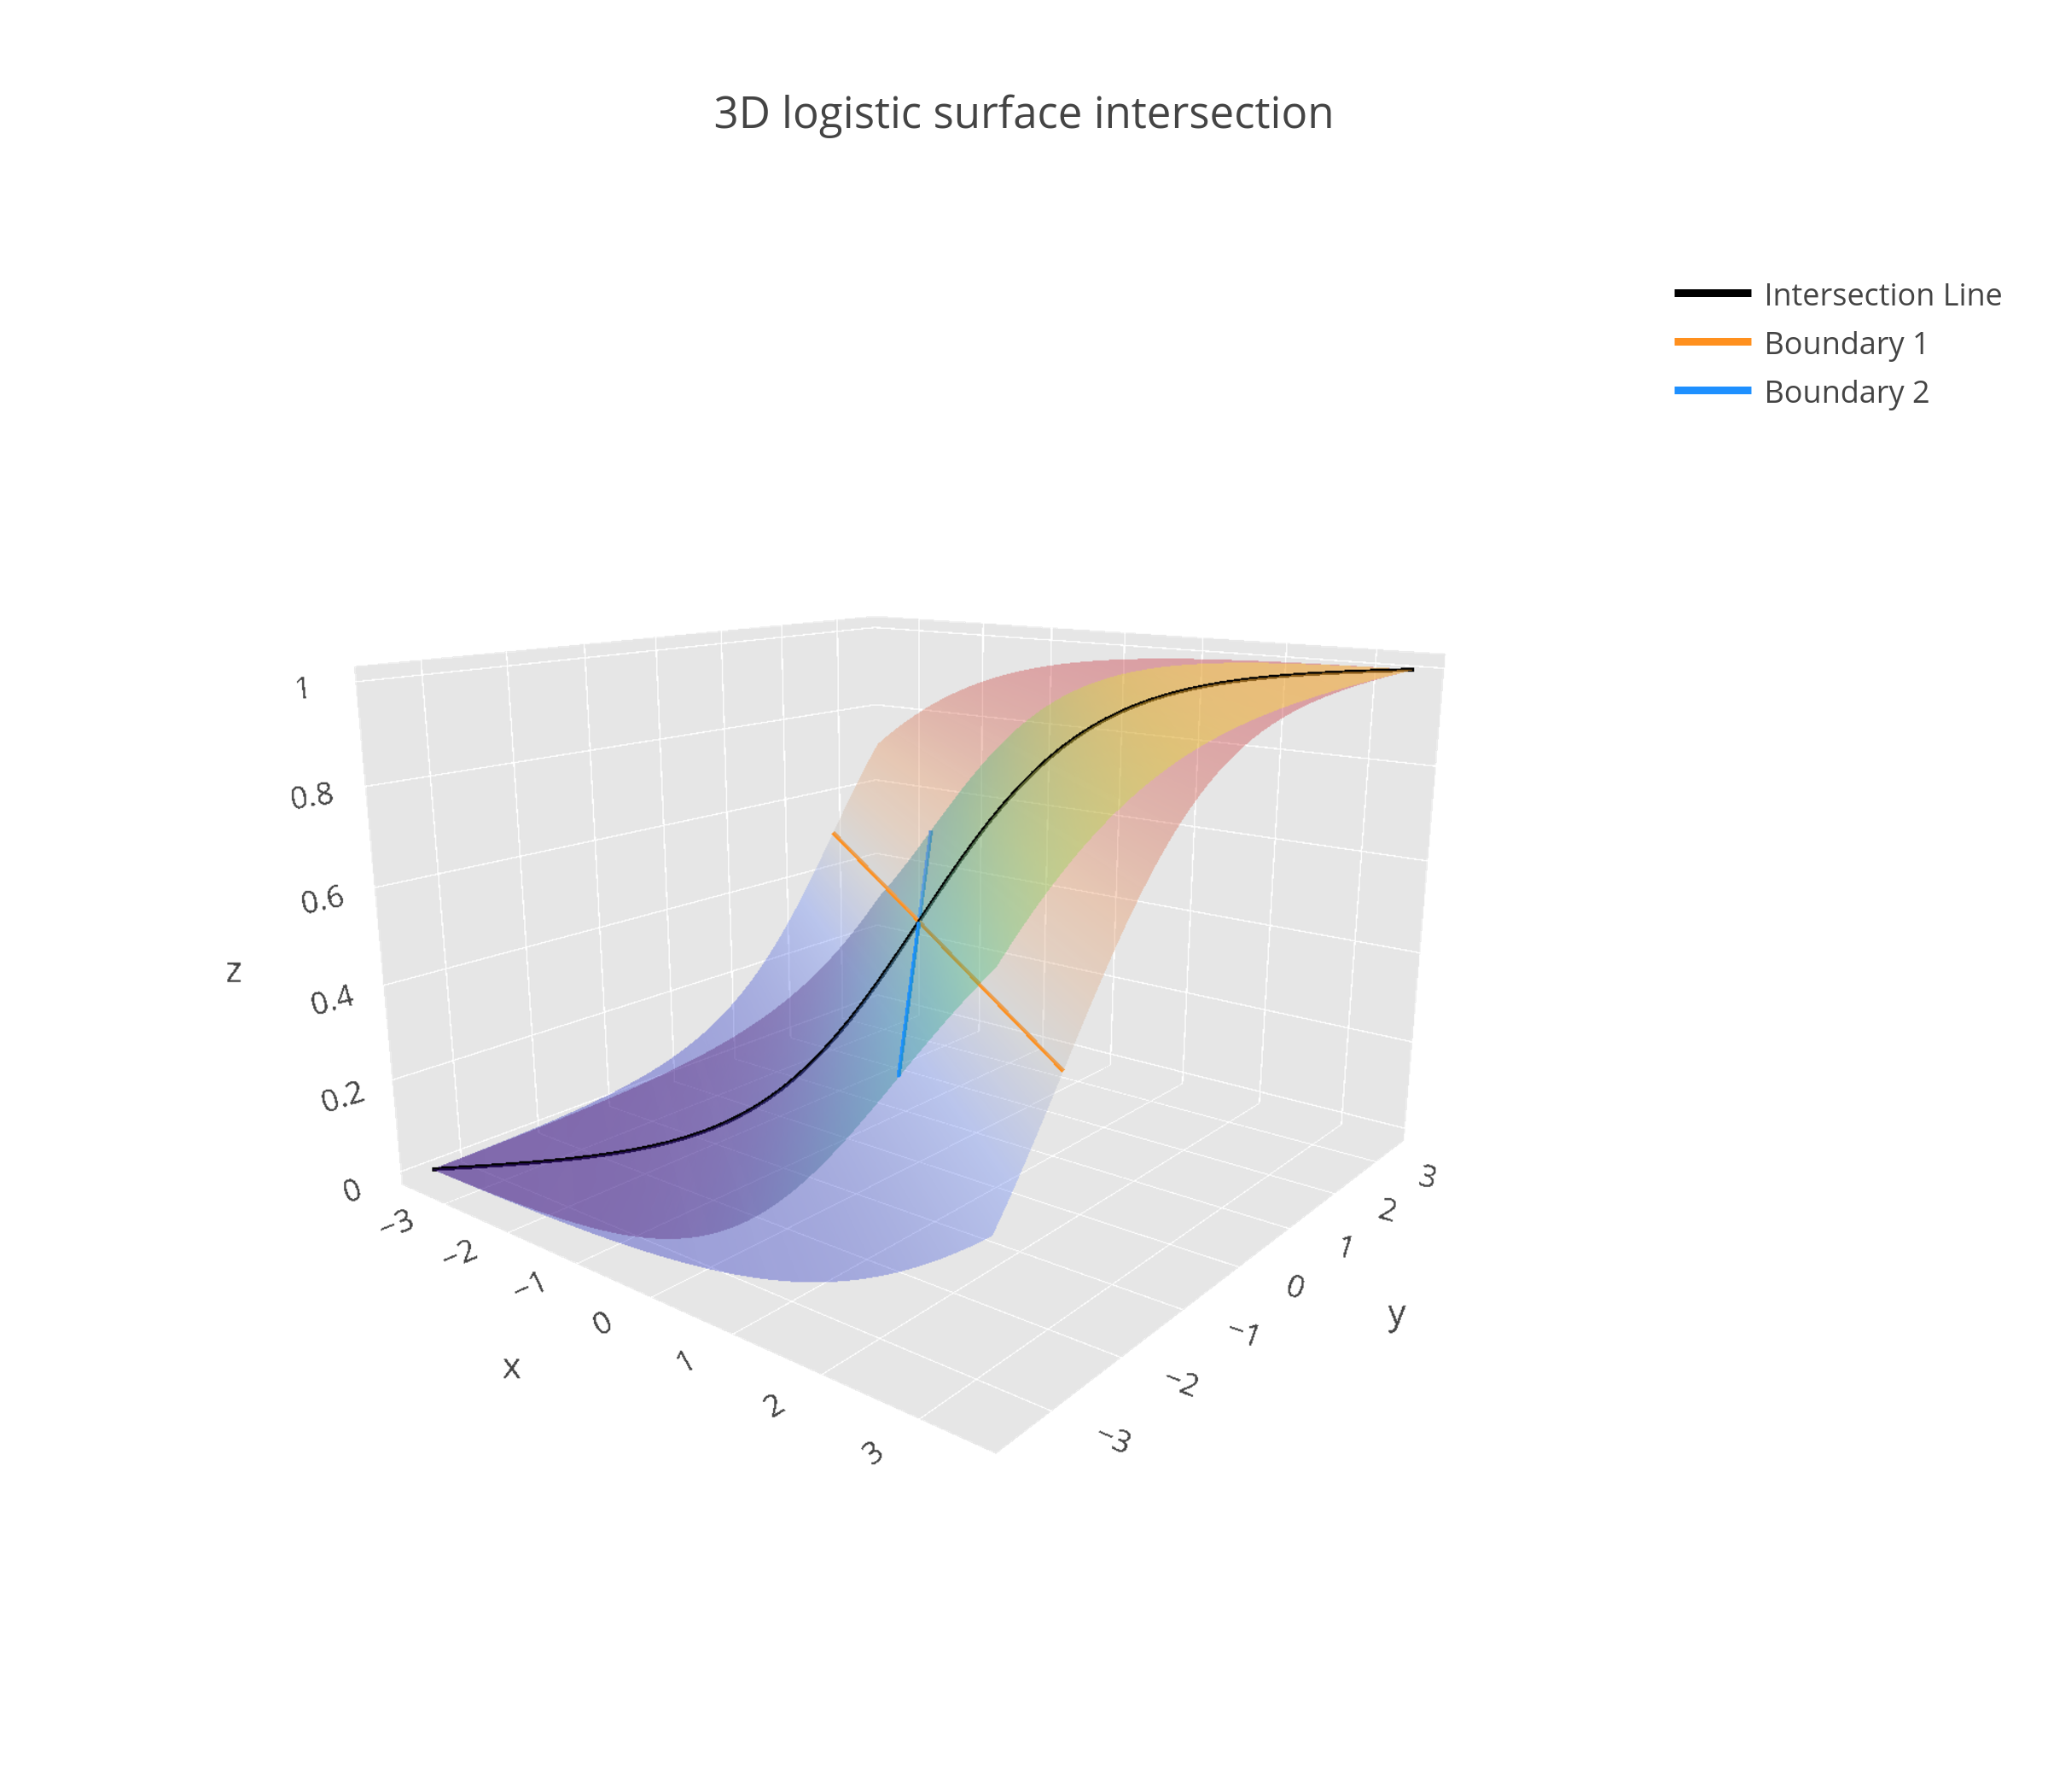
\includegraphics[width = 0.5\textwidth]{../figures/v14/demons_fig/3D_logistic_surface_intersection.png}
  \caption{The demonstration of multiple logistic regression that concept drift would result in no change in expected error rate.}
  \label{fig:logi_3d}
\end{figure}
The phenomenon observed in simple logistic regression can also be extended to multiple logistic regression. As shown in the Figure~\ref{fig:logi_3d}. Here, two logistic surfaces are plotted together, with the black line as the intersection and blue and orange lines are the optimal decision boundary for two models respectively. In this example, the error rate would not change with concept drift, because after concept drift the original model would increase local error rate in some region and decrease it in the other, resulting in zero net change in error rate. 

Besides logistic regression for binary classification data, the score-based method can also be easily applied on multi-nomial classification. 
%Besides extended to the cases with higher dimension of predictor, the score-based methods can also be applied to classification problem with more than $2$ classes, while most of methods proposed are for binary classification problems.

\subsubsection{Non-Zero Mean of Score Function with Concept Drift}
\label{ss:non_zero_mean_score}
From the discussion in the Section~\ref{ss:score_func}, the non-zero mean of score function implies concept drift. However, whether the concept drift also implies drifted mean of score function \replaced[id=Kungang, comment={Comment: This sentence results from the consideration that ``no error cannot imply no concept drift", and there are some technical assumptions related to the following statement. Also, the mean zero of score function can be achieved with concept drift when score function with different input happen to cancel each other.}]{needs justification}{is not so clear}. Here, we show that under some proper assumption, this is indeed true, which mathematically explains the superior performance of the score-based method. Generalized linear model encompasses many models used in many applications. The marginal likelihood and score function is as following:
\begin{align}
\begin{aligned}
f(y;\bm { \theta} ^{(0)}, \phi) =& \exp\{\frac{y \psi(\bm { \theta} ^{(0)})-b( \psi(\bm { \theta} ^{(0)}))}{ a ( \phi)} + c(y; \phi)\} \\
\bm {s}(\bm { \theta} ^{(0)};(\bm {X}, Y)) =& \frac{1}{a( \phi)}(y - b'( \psi (\bm { \theta})))\nabla _{ \bm { \theta}} \psi(\bm { \theta} ^{(0)})
\end{aligned}
\label{eqn:score_glm}
\end{align}
where function $b(\cdot)$ and $ \psi(\cdot)$ also depends on value of predictor $\bm { X}$, but omitted for simple notation; $ a ( \phi)$ is a positive scaling factor. In generalized linear model, $ g(E[y]) = \psi ( \bm { \theta})=\bm {x}^T\bm { \theta}$ is called link function. The expectation of the score function when $P(Y|\bm {X})$ has parameter with value $\bm { \theta} ^{(1)}$ and the change of parameter $ \Delta \bm { \theta}= \bm { \theta}^{(1)}-\bm { \theta}^{(0)}$ is small, using Taylor expansion, we can get:
\begin{align}
\begin{aligned}
E _{\bm { \theta} ^{(1)}}[\bm {s}(\bm { \theta} ^{(0)};(\bm {X}, Y))] \approx& \frac{1}{a ( \phi)}E[b''( \psi( \bm { \theta} ^{(0)}))\nabla _{ \bm { \theta}} \psi ( \bm { \theta} ^{ (0)}) \nabla _{ \bm { \theta}}^T \psi ( \bm { \theta} ^{ (0)})] \Delta \bm { \theta} \\
=& \frac{1}{a ( \phi)}E[b''( \psi( \bm { \theta} ^{(0)}))\bm {X}\bm {X}^T] \Delta \bm { \theta}
\end{aligned}
\label{eqn:exp_score_glm}
\end{align}
where the expectation without subscript is w.r.t to $\bm {X}$. It is known that $Var[y] = a ( \phi)b''(\psi ( \bm { \theta} ^{ (0)}))$ so that $b''(\psi ( \bm { \theta} ^{ (0)}))>0$ always holds, assuming response $y$ always has randomness. This indicates the matrix in the function~(\ref{eqn:exp_score_glm}) is always positive-defined if the distribution of $\bm {X}$ is not degenerated. Then, any methods for detecting multivariate mean change can be applied to this concept drift detection problem, which opens up a whole toolbox in SPC. Notice that this conclusion actually also holds when $ \psi ( \bm { \theta})$ is not a linear function of $\bm { \theta}$. For example, neural network can be used to model this function, and $\bm { \theta}$ is the vector or weights and biases of the neural net. In later simulation study, score-based method also works on neural network. 

% How to formally define detection;
% How to quantify the relationship between the rate of detection and the rate of concept drift. Any power law?
% How to quantify the relationship between the rate of detection, the rate of concept drift, and the absolute value of concept drift. Any power law?
% After carefully define and quantify detection of concept drift in the simplest case, we can start to think about the online learning rate of more complex concept drift pattern. For example, when we have an alternative concept drift pattern. How should we choose statistics to monitor to get a better estimation of parameters in concept drift. In the online training context, early detection and change learning rate according maybe a way to solve concept drift problem better.

\subsection{Monitoring Sample Score Vectors with the High-Dimension Vector of Parameters}
One of the advancement of machine learning is that models become increasingly complex. Some models can have millions of parameters, like convolutional neural network. To monitor those models for concept drift, we can calculate sample score vectors when we make prediction or finely tune models. However, with such high-dimension of parameters, the inverse of the sample covariance matrix in (\ref{eqn:hotellingt2}), $\hat {\bm { \Sigma}}_t$, is very likely to be singular. For example, when the sample size of our training data (denoted as $N_1$ as in the Section~\ref{ss:comp_other_metrics}) is smaller than the dimension of parameters, $dim(\bm { \theta})$, the sample covariance would be singular. 

To solve this problem, we can add a nugget parameter on all diagonal entries of $\hat {\bm { \Sigma}}_t$ or use pseudo-inverse of the sample covariance. For the method of adding a nugget parameter $ \delta$, we assign $\hat {\bm { \Sigma}}_t+ \delta \bm {I}$ to $\tilde {\bm { \Sigma}}_t$ as the approximated covariance matrix. To understand the effect of this nugget parameter, denote the eigen-decomposition of the sample covariance matrix as $\hat {\bm { \Sigma}}_t = \bm {Q}\bm { \Lambda} \bm {Q}^T$ and obtain the eigen-values as $ diag(\bm{\Lambda}) = [ \lambda_1, \lambda_2,\cdots, \lambda_n]$ in a non-increasing order. Then, we can write the approximated sample covariance matrix as $\tilde {\bm { \Sigma}}_t = \bm {Q}\tilde{\bm { \Lambda}} \bm {Q}^T$, where $\tilde{\bm { \Lambda}} = \bm { \Lambda} + \delta \bm {I}$. The EWMA of the new statistics with this modified covariance matrix in the equation~(\ref{eqn:hotellingt2}) bypasses the issue of ill-conditioning by suppressing unimportant directions of variation. 

Setting a condition number achieves a similar purpose. By setting a maximum condition number, $ \gamma$, we set all $ \lambda_i$ equal to $0$, if $ \lambda_1 \geq \gamma \lambda_i$. Denote the maximum of the index of $ \lambda_i$ which is not set to $0$ as $k$ and a new diagonal matrix $\bm { \Lambda} ^{-}$ as $diag(\bm { \Lambda} ^{-}) = [1/\lambda_1,1/\lambda_2, \cdots, 1/\lambda_k, 0, \cdots, 0]$. Then, a pseudo-inverse of the sample covariance matrix is defined as $\hat {\bm { \Sigma}}_t ^{-} = \bm {Q}\bm { \Lambda}^{-}\bm {Q}^T$. This is equivalent to applying PCA onto $\bm {z}_t$, so that the most important variations in $\bm {z}_t$ are kept. 

Comparing with adding a nugget parameter, even though both methods give similar results, setting the maximum condition number is more intuitive in terms of controling the behavior of inverting the covariance matrix, while adding the nugget allows the concept drift to be detected in those directions, that would be otherwise set to $0$ in hard thresholding by setting the maximum condition number. So we choose to add a nugget parameter.

\subsection{Score function of Penalized Models}
In many current applications, models become increasingly complex, which almost always require penalization to combat overfitting. The penalty term would change the score function of the original model. The penalization term can be looked as a prior on parameters from Bayesian perspective. Then, we can simply ``distribute" the prior among all data and treat the likelihood times prior as the new model. Then, all methods of calculating score vectors and applying EWMA and Hotelling $T^2$ follows. In some popular form of penalization, this would not change the monitoring statistics. For example, adding a $l_2$ penalization term of all parameters would only add a constant vector to all score vectors. Adding penalization would have another good effect. When $dim ( \bm { \theta})$ is too large, $l_2$ penalization would add a diagonal matrix with positive entries to the sample covariance matrix, automatically resulting in a well-conditioned matrix. We will encounter a penalization in neural network models. 

% Here another way is use pseudo-inverse.
\section{Decoupling of Concept Drift for Multivariate Regression and Classification}
\label{s:decou_cd}
While detecting the concept drift, we want to pinpoint which {covariates} have significant impact on the change of {the} conditional distribution {$P(Y| \bm {X}, \bm{\theta})$}. This can provide interpretability for concept drift for updating or fixing models. In some industry (e.g. financial, insurance, manufacturing), model interpretability is valued or even required by laws. Ideally, after decoupling, univariate control charts should truly reflect whether covariates have concept drifts or not. However, even for those covariates without concept drifts, the variance would increases due to variance of $\bm {X}$. More detailed analysis will follow in this section.

\subsection{Concept Drift Decoupling}
To detect which covariates have concept drift, naively monitoring component-wise mean {drift} of the score function breaks down when {covariates considerably correlate with each other} or nonlinear predictive models are used. To demonstrate this, look at linear model and logistic regression. Assuming the vector of the true parameters {before concept drift $\bm { \theta}^ { (0)}$} is known (we ignore the difference between the true parameter, $\bm { \theta}^ { (0)}$, and the estimator of it, $\hat{\bm { \theta}}$, as discussed in the Section~\ref{ss:sgd_score}), the linear regression and the corresponding score function implies that {$E_{\bm{ \theta}^{ (0)}}[(Y - \bm {x}^T\bm { \theta}^{ (0)} ) \bm {X}|\bm {X}]=0$}. Note the notation that, the subscript, ${ \bm{\theta}}^{ (0)}$, of the expectation is the vector of parameters of the underlying distribution the expectation is taken w.r.t., and the $\bm{ \theta}^{ (0)}$ in the expectation is the value taken for that vector. The two can be different, when the mean drift of concept drift is derived. After concept drift, {assuming the parameter $\bm { \theta}^{ (0)}$ changes to $\bm { \theta} ^{ (1)}$, denote the change in the vector of parameters as $ \Delta \bm { \theta} = \bm { \theta} ^{ (1)} - \bm { \theta}^ { (0)}$ for the rest context.} {The} joint expectation for the score function is $E [\bm {X}\bm {X}^T] \Delta \bm { \theta}$, where the concept drift only decouples when $E [\bm {X}\bm {X}^T]$ is an {diagonal} matrix. For logistic regression, the joint expectation of the score function, $E[(\sigma ( \bm {  \bm {X}^T \theta}^{ (1)}) - \sigma ( \bm {X}^T\bm { \theta}^{ (0)} )) \bm {X}]$,  no longer has a clean format, because it depends on the unknown parameter vector, $\bm { \theta} ^{ (1)}$, after concept drift. In the next section, results from simulated data show that this mean {drift} is not decoupled even when $X _{i} (i = 1,2, \cdots, p)$ are uncorrelated. 

To decouple the interleaved drifts of parameters, for linear regression, we can simply premultiply sample score vectors by the {the inverse of the estimated} $E [\bm {X}\bm {X}^T]$, because this matrix doesn't depend on the actual drift in parameters (otherwise, it is generally hard to estimate when concept drift starts). However, this is not universally viable for more complex models, like in logistic regression. In general, the mean {drift} of the score function after concept drift is
\begin{align}
\begin{aligned}
E _{\bm { \theta}^{ (1)}}[\bm{s}(\bm { \theta}^{ (0)}; (\bm {X}, Y))] 
= & E[E _{\bm { \theta}^{ (1)}}[\bm{s}(\bm { \theta}^{ (0)}; (\bm {X}, Y))| \bm {X}] ] \\
= & E[\int _{y}\bm{s}(\bm { \theta}^{ (0)}; (\bm {X}, y)) P(y | \bm {X}, \bm{\theta} ^{ (1)}) dy ]
\end{aligned}
\label{eqn:cd_mean_shift}
\end{align}
Apply Taylor expansion on the $\bm{s}(\bm { \theta}^{ (0)}; (\bm {x}, y))$ around $\bm { \theta} ^{ (1)}$
\begin{align}
\begin{aligned}
 &\bm{s}(\bm { \theta}^{ (0)}; (\bm {x}, y)) = \bm{s}(\bm { \theta}^{ (1)}; (\bm {x}, y)) 
 + \nabla _{\bm { \theta}}{ \bm{s}(\bm { \theta}^{ (1)}; (\bm {x}, y))}(\bm { \theta}^ { (0)} - \bm { \theta} ^{ (1)}) 
 + o(\bm { \theta}^ { (0)} - \bm { \theta} ^{ (1)} ) 
\end{aligned}
\label{eqn:sc_ty_expa}
\end{align}
Substitute equation (\ref{eqn:sc_ty_expa}) into (\ref{eqn:cd_mean_shift}) and use the property of the score function for $\bm { \theta} ^{ (1)}$.
\begin{align}
\begin{aligned}
& E _{\bm { \theta}^{ (1)}}[\bm{s}(\bm { \theta}^{ (0)}; (\bm {X}, Y))] \\
= & E[\int _{y} \bm{s}(\bm { \theta}^{ (1)}; (\bm {X}, y))P (y| \bm {X}, \bm{\theta}^{ (1)}) d y ] \\ 
 +&  E[\int _{y} [  \nabla _{\bm { \theta}}{ \bm{s}(\bm { \theta}^{ (1)}; (\bm {x}, y))}(\bm { \theta}^ { (0)} - \bm { \theta} ^{ (1)}) \\ 
 +& o(\bm { \theta}^ { (0)} - \bm { \theta} ^{ (1)} ) ] P (y| \bm {X}, \bm{\theta}^{ (1)}) d y]\\ 
= & E[E _{\bm { \theta}^{ (1)}}[\bm{s}(\bm { \theta}^{ (1)}; (\bm {X}, Y))| \bm {X}]] \\
+ & E[\int _{y} [ \nabla_{\bm { \theta}} \nabla^T _{\bm { \theta}}{ \ln f(\bm { \theta}^{ (1)}| (\bm {x}, y))}(\bm { \theta}^ { (0)} - \bm { \theta} ^{ (1)}) \\
+ & o(\bm { \theta}^ { (0)}- \bm { \theta}^{ (1)})]P (y| \bm {X}, \bm{\theta}^{ (1)}) dy] \\
= & \bm{0} +  \{E[E _{\bm { \theta}^{ (1)}}[\nabla_{\bm { \theta}} \nabla ^T_{\bm { \theta}}{ \ln {f}(\bm { \theta}^{ (1)}| (\bm {x}, y))} | \bm {X}]] \\ + &o(1)\}(\bm { \theta}^{ (1)} - \bm { \theta}^ { (0)}) \\
= & [{\mathbf {I}}(\bm { \theta}^{ (1)})+ o(1)](\bm { \theta}^{ (1)} - \bm { \theta}^ { (0)}) \\
= & [{\mathbf {I}}(\bm { \theta}^{ (0)})+ o(1)](\bm { \theta}^{ (1)} - \bm { \theta}^ { (0)}) \\
%= & (\bm { \theta}^ {tr} - \bm { \theta}^{dr}) \int \left.\frac{\partial^2 \ln f (y | \bm {x}, \bm{\theta})}{\partial \bm { \theta}\partial \bm { \theta}^T}\right| _{\bm { \theta} = \bm { \theta}^{'}} f (y | \bm {x}, \bm{\theta}^{'}) d y \\
%+ & o(\bm { \theta}^* - \bm { \theta}^{'})  \\
%= & {\mathbf {I}}(\bm { \theta}^{'}|\bm {x})(\bm { \theta}^{'} - \bm { \theta}^*) + o(\bm { \theta}^* - \bm { \theta}^{'})  \\
%= & {\mathbf {I}}(\bm { \theta}|\bm {x})(\bm { \theta}^{'} - \bm { \theta}^*) + o(\bm { \theta}^* - \bm { \theta}^{'})
\end{aligned}
\label{eqn:fisher_approx}
\end{align}
where {${\mathbf {I}}(\bm { \theta}^{ (0)})=E[E _{\bm { \theta}^{ (0)}}[\nabla_{\bm { \theta}} \nabla^T _{\bm { \theta}}{ \ln{f}(\bm { \theta}^{ (0)}; (\bm {x}, y))} | \bm {X}]]$} is the (expected) Fisher Information Matrix {at parameter $\bm { \theta} ^{ (0)}$} and $o(\cdot)$ represents asymptotically negligible quantity comparing with the argument. Here, we use the fact that the expectation of the score function is $\bm {0}$ when {$\bm { \theta}^{ (1)}$} is true and assume {$ \bm { \theta}^ { (1)} - \bm { \theta}^{ (0)} $} small. To approximately decouple concept drift, we can premultiply sample score vectors by {the} inverse of {the} estimated {${\mathbf {I}}(\bm { \theta}^{ (0)})$}, or the sample covariance matrix of {the score function.}

\subsection{Variance Inflation for Covariates without Concept Drift}
\label{ss:var_infla}
\added[id=Kungang, comment={}]{Notice that the expectation in (\ref{eqn:score_exp_zero}) is w.r.t. the conditional distribution, but the sample score vector, {$\bm{s} (\bm { \theta} ^{ (0)};(\bm {x}_i, y_i))$}, has randomness from not only $P_{\bm {\theta}} (Y|\bm {X})$ (where $\bm { \theta} = \bm { \theta}^{(0)}$ when no concept drift) but also $P (\bm {X})$. In other words, monitoring mean {drift} of {$\bm{s} (\bm { \theta}^{ (0)};(\bm {x}_i, y_i))$} using control charts (which will be formally introduced later) is practically implemented by monitoring drift of {$E _{ \bm { \theta}}[\bm{s} (\bm { \theta}^{ (0)};(\bm {X}, Y))]$}.
%\begin{align}
%\begin{aligned}
%&E _{\bm { \theta}^{tr}}[\bm{s}(\bm { \theta}^{tr}| (\bm {X}, Y))| \bm {X}=\bm {x}] \\
%= & \int _{y}\bm{s}(\bm { \theta}^{tr}| (\bm {x}, y)) p(y | \bm {x}, \bm{\theta} ^{tr}) dy\\
%= & \int _{y}\bm{s}(\bm { \theta}^{tr}| (\bm {x}, y)) f(\bm{\theta}^{tr}| (\bm {x},y)) dy = \bm {0}
%\end{aligned}
%\label{eqn:expe_score}
%\end{align}
To understand the relation, using iterative expectation, we have}
\begin{align}
E_{ \bm { \theta} }[\bm{s} (\bm { \theta} ^{ (0)};(\bm {X}, Y))] = E [E _{ \bm { \theta} }[\bm{s} (\bm { \theta} ^{ (0)};(\bm {X}, Y)); \bm {X}]]
\label{eqn:joint_expe}
\end{align}
\added[id=Kungang, comment={}]{According to the definition, a concept drift corresponds to change in $E _{ \bm { \theta} }[\bm{s} (\bm { \theta} ^{ (0)};(\bm {X}, Y))| \bm {X}]$ from $\bm{0}$, because this indicates the change in $P(Y|\bm {X})$. In practice, we can not directly monitor $E _{ \bm { \theta} }[\bm{s} (\bm { \theta} ^{ (0)};(\bm {X}, Y))| \bm {X}]$, because of lack of control in randomness from $\bm {X}$. Instead, we actually monitor $E_{ \bm { \theta} }[\bm{s} (\bm { \theta} ^{ (0)};(\bm {X}, Y))]$. This actually makes sense, because the {drift} of the left-hand-side in (\ref{eqn:joint_expe}) implies the {drift} of inner expectation of the right-hand-side, meaning concept drift; the reverse is generally true except that {$E _{ \bm { \theta} }[\bm{s} (\bm { \theta} ^{ (0)};(\bm {X}, Y))| \bm {X}]$} has a specific form and non-zero values at different realizations of $\bm {X}$ cancel out after taking expectation w.r.t. $\bm {X}$. As shown in Section~\ref{ss:non_zero_mean_score}, under assumption of small changes and smooth conditions w.r.t the parameter, for generalized linear model, concept drift in parametric models implies non-zero mean of score function.}

As mentioned before, the univariate score function corresponding to those covariates without concept drifts will have $\bm{0}$ mean in univariate control charts, but the variance would be inflated if concept drifts exist in other covariates so that the monitored statistics will still fall outside of control limits. Because of the clear pattern without mean drifts, these components should not be included as candidates of origins of concept drifts, and after recovering those covariates from concept drifts as required by some applications, the inflated variance in control charts should go back to normal. To give an example here, linear regression is used to show the origin of variance inflation.

For a linear regression mode, assuming that the data generation model is $y' = \bm {x}^T\bm { \theta}^{ (1)} + \epsilon$, the variance of the $k$th component after the concept drift is
%\begin{align}
%\begin{aligned}
%&Var _{\bm{ \theta}^{(0)}}[ (Y- \bm {X}^T\bm{ \theta}^{(0)}) X_{k}]  \\
%= & E _{ \bm{ \theta}^{(0)}} [(Y-   \bm {X}^T\bm{ \theta}^{(0)})^2 X_{k}^2] - E _{ \bm{ \theta}^{(0)}}^2 [(Y- \bm {X}^T\bm{ \theta}^{(0)} ) X_{k}]  \\
%= & E _{\bm{ \theta}^{(0)}} [(Y - \bm {X}^T\bm{ \theta}^{(0)})^2 X_{k}^2]  \\
%= & E [E _{\bm{ \theta}^{(0)}}[(Y - \bm {X}^T\bm{ \theta}^{(0)} )^2| \bm {X}] X_{k}^2]  \\
%= & \sigma^2 E[  X_{k}^2] = \sigma^2 \sigma_{x,k}^2
%\end{aligned}
%\label{eqn:var_bef_cd}
%\end{align}
\begin{align}
\begin{aligned}
&Var _{ \bm{ \theta}^{(1)}}[ (Y'- \bm {X}^T \bm{\theta}^{(0)}  ) X_{k}]   \\
%= & E  [Var  _{ \bm{ \theta}^{(1)}}[(Y' - \mu ) X_{k}]] + Var  [E  _{ \bm{ \theta}^{(1)}}[(Y' - \mu ) X_{k}]]   \\
%= & 
= & E _{\bm{ \theta}^{(1)}} [(\bm {X}^T \bm{\theta}^{(1)}+\epsilon -  \bm {X}^T \bm{\theta}^{(0)}  )^2 X_{k}^2] - E _{\bm{ \theta}^{(1)}}^2 [(\bm {X}^T \bm{\theta}^{(1)}+\epsilon - \bm {X}^T \bm{\theta}^{(0)}) X_{k}]   \\
= & E   [E _{\bm{ \theta}^{(1)}}[(\bm {X}^T\Delta \bm { \theta}  +\epsilon)^2|\bm {X}] X_{k}^2] - \Delta \bm{\theta}^T E   [\bm {X}  X_{k}]E   [\bm {X} ^T X_{k}] \Delta \bm { \theta}    \\
= & E   [ (\Delta \bm { \theta}^T \bm {X} \bm {X} ^T \Delta \bm { \theta} + \sigma^2)X_{k}^2] - \Delta \bm{\theta}^T E   [\bm {X}  X_{k}]E   [\bm {X} ^T X_{k}] \Delta \bm { \theta}    \\
= & \sigma^2 \sigma_{x,k}^2 + \Delta \bm{\theta}^TVar [\bm {X}  X_{k}] \Delta \bm{\theta}
\end{aligned}
\label{eqn:var_aft_cd}
\end{align}
where $ \sigma$ is the variance of random noise and $ \sigma _{x,k}$ is the variance of the $k$th component of the predictor variable. Clearly, $\Delta \bm{\theta}^TVar [\bm {X}  X_{k}]\Delta \bm{\theta}$ is generally non-zero if $ \Delta \bm { \theta} \neq \bm {0}$, resulting in variance inflation for predictor without concept drift. Notice that because the variance of lines in control charts depends on the predictor variable, ``covariate drift" (meaning change in distribution of $\bm {X}$) will also affect the variance in the control charts, but not mean. In this study, we assume no covariate drift.

\section{Demonstration of Monitoring the Score Function}
The concept drift in real datasets is notoriously hard to testify unless there is some strong prior knowledge on when drifts happened. To test the properties mentioned in the Section~\ref{s:decou_cd}, we first use simulated datasets. Here, we focus on simple but commonly used models like linear model, logistic regression, multinomial regression, poisson regression, and MLP, for the simplicity of proof-of-concept and analytical explanation. We expect that those properties can be extended to more complex models, because our previous analyses on the score function are mostly model and distribution agnostic. 

In the following demonstration and analysis, several experiments are shown the efficacy and properties of score-based method and its superior performance comparing with other metrics. First, simulations shown that concept drift can result in no expected error rate change (thus no detection) on control charts, but large mean drift in score. Then, Monte Carlo simulation experiments are conducted to calculate Median Run Length ($MRL$) for both in-control and out-of-control regions, showing that score-based method have higher sensitivity in detection. At the last, datasets with partially correlated covariates are simulated to show that score-based method can decouple the concept drift, with proper scaling.
%The generated datasets have independent or correlated covariates to illustrate the effect of decoupling operations and under which conditions they can be useful. Because the most of real datasets have more or less multicollinearity, more emphasis is put on datasets having correlated covariates. 
We also simulate abrupt and gradual concept drifts to test the performance of detecting and tracking concept drifts by monitoring the score function, as well as other metrics like EWMA of the prediction error or absolute residual. Those results show that monitoring the score function is a better and more versatile method in solving with concept drift problems. 

\subsection{Concept Drifts with No Error Rate Change}
\begin{figure}[!htp]
\centering
\begin{subfigure}[t]{0.49\linewidth}
         \centering
        %   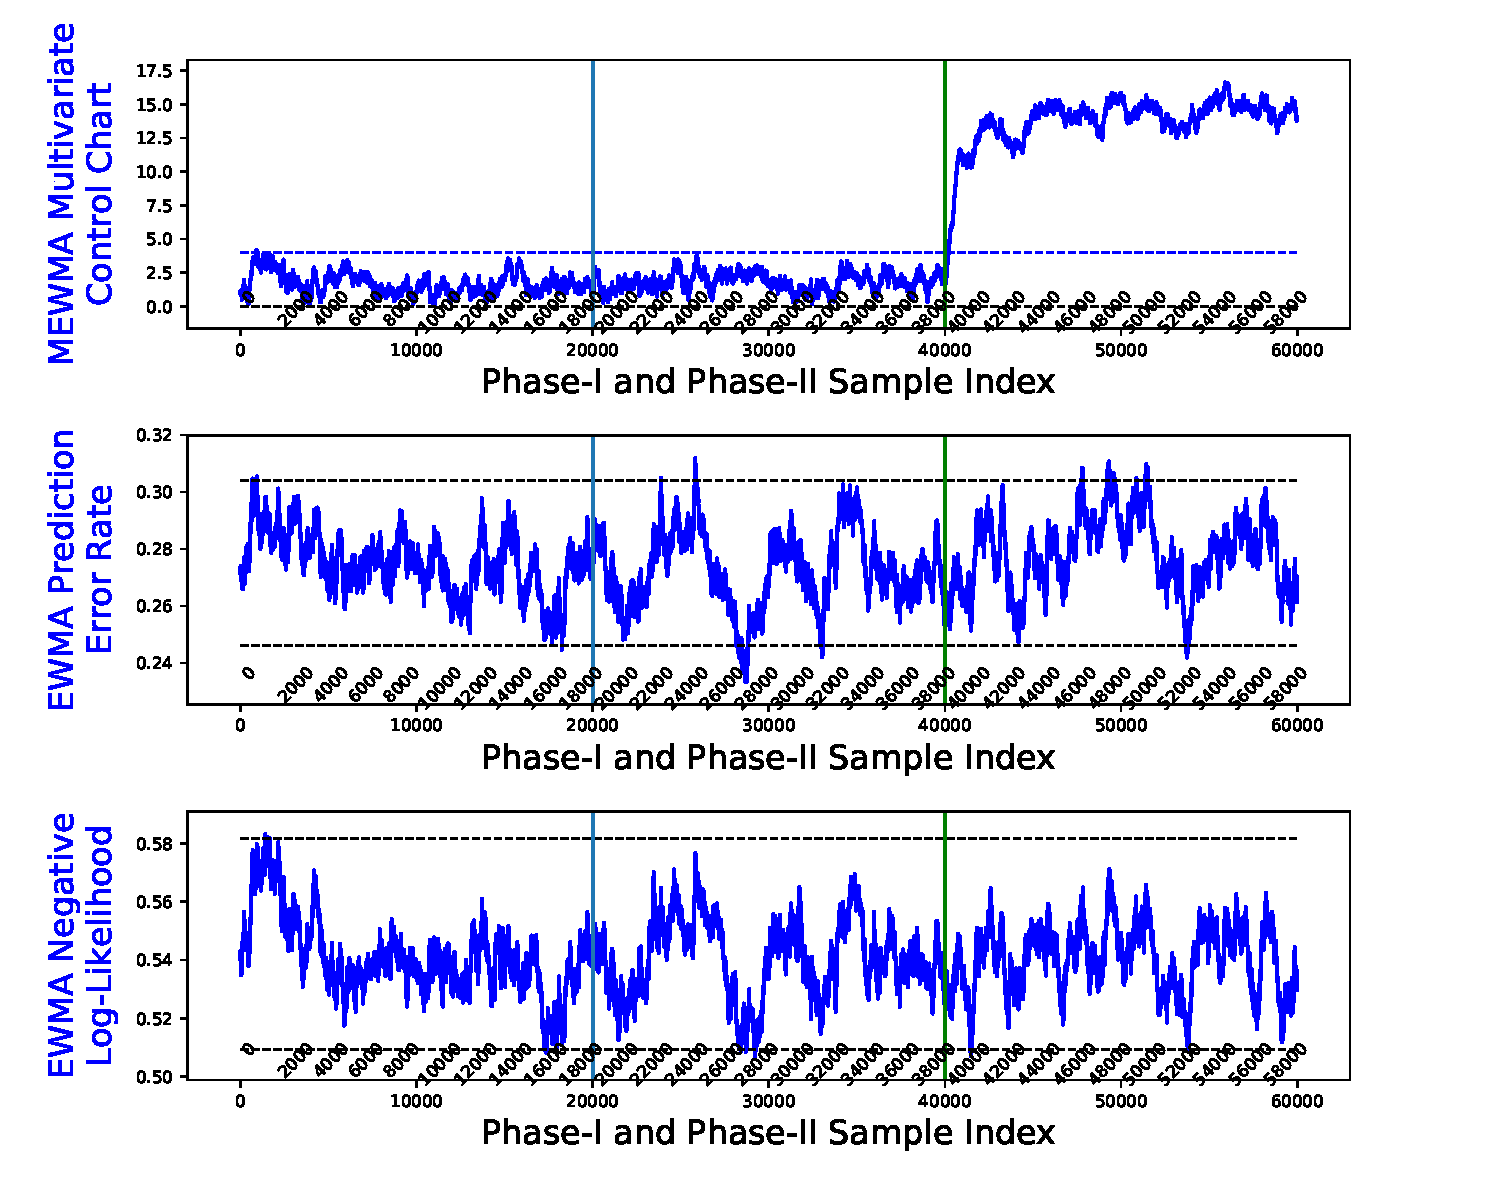
\includegraphics[width = \linewidth, trim=0in 2.6in 0in 0in, clip]{../figures/v14/sim_11/non_nnet_unif_ch_f_trans/1_sim11_logi_1e-08_0_0015_1.png}
           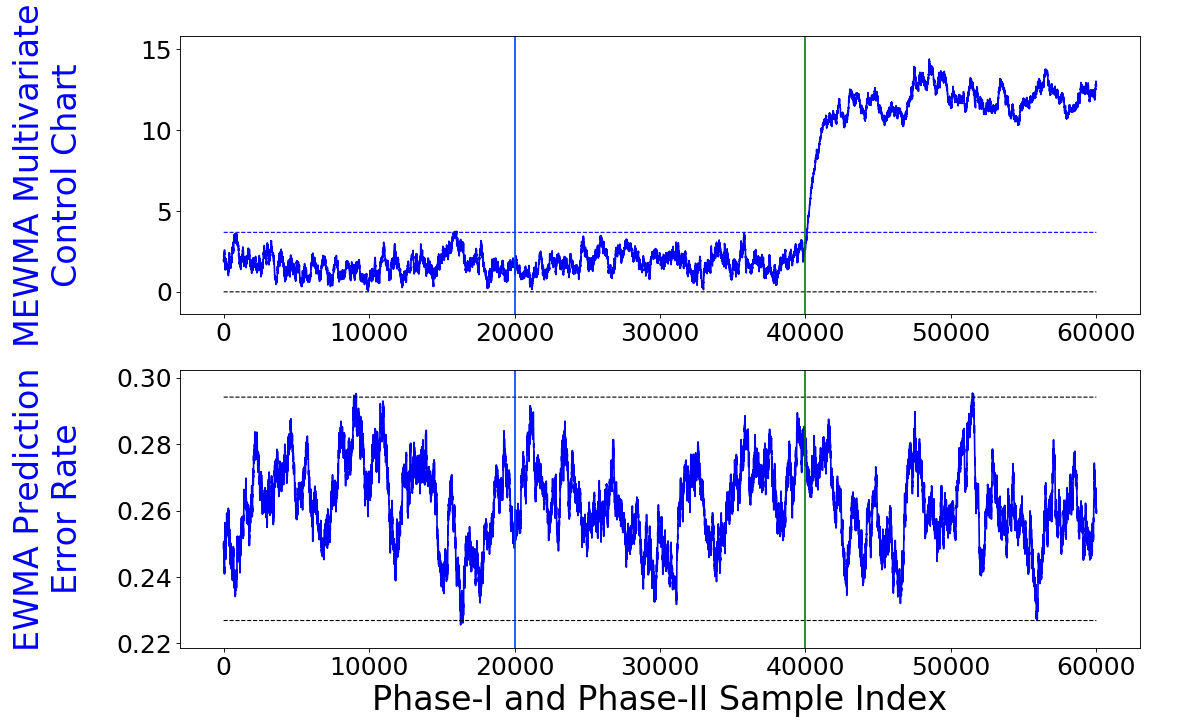
\includegraphics[width = \linewidth]{../figures/v14/sim_11/non_nnet_nonunif_ch_f_0_2/1_sim11_logi_1e-08_0_0015_1.png}
         \caption{Concept drift results mean change in score-based method but no mean change in error rate.}
         \label{fig:exp_no_err_ch_a}
  \end{subfigure}
\begin{subfigure}[t]{0.49\linewidth}
         \centering
	       %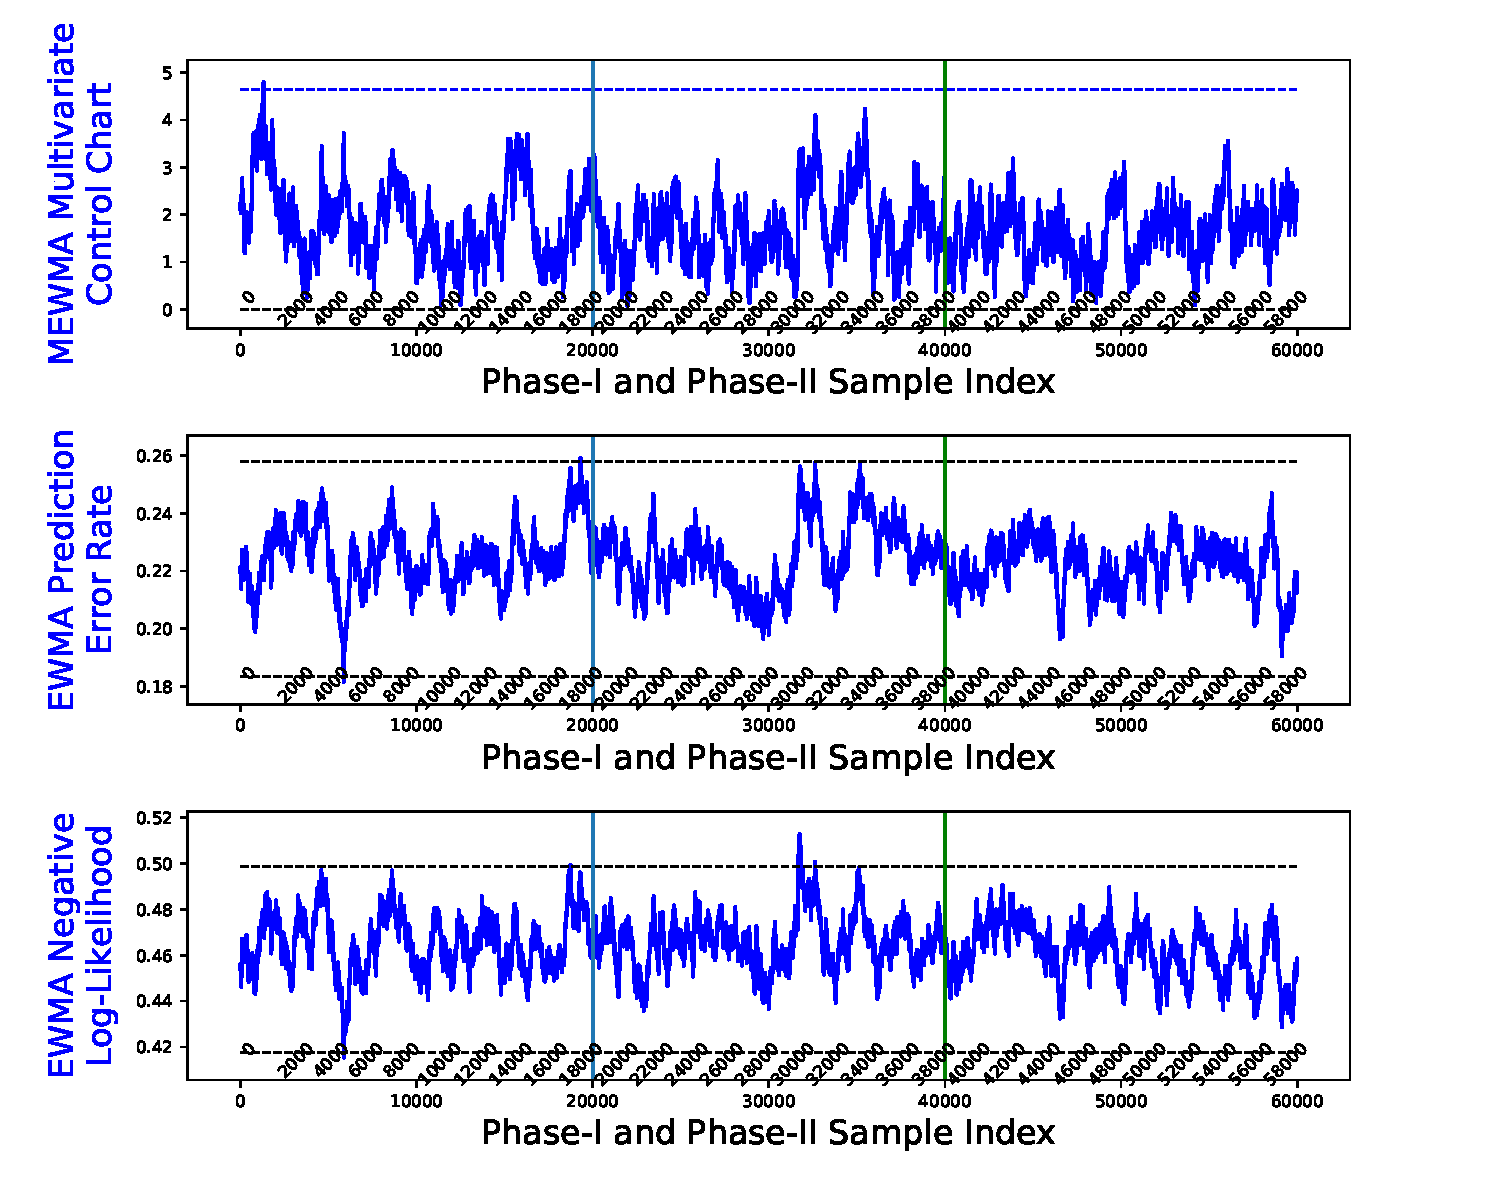
\includegraphics[width = \linewidth, trim=0in 2.6in 0in 0in, clip]{../figures/v14/sim_11/non_nnet_unif_ch_f_trans_followup/1_sim11_logi_1e-08_0_0015_1.png}
	       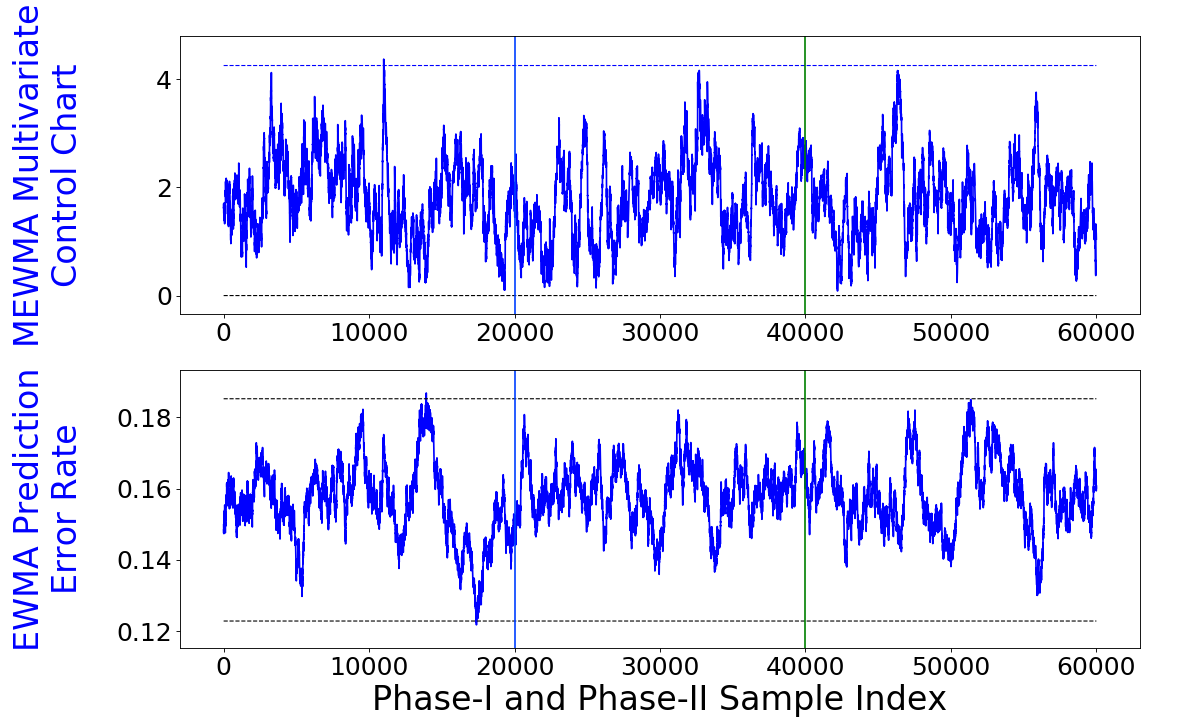
\includegraphics[width = \linewidth]{../figures/v14/sim_11/non_nnet_nonunif_ch_f_0_2_followup/1_sim11_logi_1e-08_0_0015_1.png}
         \caption{After retrained on the drifted dataset, the performance of model increased, according to lower limits in prediction error.}
         \label{fig:exp_no_err_ch_b}
  \end{subfigure}
%  \includegraphics[width = 0.8\linewidth]{../figures/sim_2_pinv_pdf/sim2_ewma_2_metric_with_reg_1e-08_0_005.png}
%  \includegraphics[width = 0.48\linewidth]{../figures/sim_2_pinv/sim2_ewma_log_lik_with_reg_1e-08_0_005.png}
  \caption{A logistic regression example with two covariates, where before blue vertical line is Phase-I and the green vertical line is the boundary between concept drift in the Phase-II. This example shows that score-based method can detect concept drift which has no change in error. This detection provides an opportunity for improvement as shown in the lower limits on the right plot.}
  \label{fig:exp_no_err_ch}
\end{figure}
In the Section~\ref{ss:comp_other_metrics}, simple logistic regression has been shown that concept drift may not result in mean change in expected error rate which defeats the purpose of detecting and monitoring it. Here, for a simple demonstration, we simulate Bernoulli datasets with two covariates. The concept drift is similar as shown in the Figure~\ref{fig:logi_err_rate_unch}. As shown in the Plot~\ref{fig:logi_err_rate_unch_a}, prediction error rate has no significant signal for successful detection on concept drift. However, the score-based method shows large deviation. After retraining model over drifted dataset, the results shown in the Plot~\ref{fig:logi_err_rate_unch_b} indicate that the accuracy has been increased because of lower control limit on prediction error rate. This example directly proves that score-based method has advantage over error-based method. 

\subsection{Simulations on Median Run-Length ($MRL$)}
\label{ss:simu_MRL}
To quantitatively show higher sensitivity of score-based method, the Monte Carlo simulations are conducted for different models to calculate $MRL$. Datasets are generated according to linear, logistic, multinomial, and poisson regression. Then, corresponding training models are obtained by learning through those simulated datasets.

For a fair comparison, error rate, residual, and score-based metrics are applied with EWMA with the same parameter $\lambda$, as defined in the Section~\ref{ss:MEWMA}. In SPC, different change sizes have different optimal $ \lambda$'s, because of the trade-off of sensitivity in change size and detection delay. Here, we choose three change sizes and $ \lambda$'s so that $MRL_0$ (in-control $MRL$) are equal to a given value. The shorter $MRL_1$ (out-of-control $MRL$) for a given $ \lambda$, the concept drift is detected earlier. Here, examples of linear(Table~\ref{tab:lin_MRL}), logistic(Table~\ref{tab:logi_MRL}), multinomial(Table~\ref{tab:multi_logi_MRL}), and poisson(Table~\ref{tab:pois_MRL}) regressions are tested. The neural network models (Table~\ref{tab:lin_nnet_MRL},~\ref{tab:logi_nnet_MRL},~\ref{tab:multi_logi_nnet_MRL}) are also applied on those datasets to see if score-based method can also be used in highly nonlinear models. In those tables, $ \alpha$ is the changing factor that represents the size of concept drift or changes of parameters (larger $ \alpha$ means larger concept drift). As shown in results, score-based method has smaller $MLR_1$, which indicates higher sensitivity. The gap between $MRL_1$ of score-based metric and other metrics is larger when concept drift size is smaller, that is the detection becomes more challenging. Those simulations prove the generality and superior capability of score-based method.

\begin{table}[!t]
\centering
\begin{tabular}{ccccc}
\toprule
\multicolumn{2}{c}{($ \alpha$, $ \lambda$)} & {$  \lambda_1$} & {$ \lambda_2$} & {$ \lambda_3$} \\
\midrule
\multirow{3}{*}{$\alpha = 0$} & score &$3500.0$ & $3499.0$ & $3502.5$ \\
& err &$3499.5$ & $3501.0$ & $3500.0$ \\
%& dev &$3499.5$ & $3499.5$ & $3501.0$ \\
\midrule
\multirow{3}{*}{$\alpha = 0.3$} & score &$\bm{391.0}$ & $\bm{377.5}$ & $\bm{464.0}$ \\
& err &$835.0$ & $1050.0$ & $1278.0$ \\
%& dev &$575.0$ & $633.0$ & $814.0$ \\
\midrule
\multirow{3}{*}{$\alpha = 0.5$} & score &$\bm{184.0}$ & $\bm{148.0}$ & $\bm{153.0}$ \\
& err &$359.0$ & $360.5$ & $442.0$ \\
%& dev &$244.0$ & $218.0$ & $239.0$ \\
\midrule
\multirow{3}{*}{$\alpha = 0.7$} & score &$\bm{111.0}$ & $\bm{82.0}$ & $\bm{75.0}$ \\
& err &$205.0$ & $177.0$ & $186.0$ \\
%& dev &$134.0$ & $108.0$ & $105.0$ \\
\midrule
\end{tabular}
\caption{Comparison of Phase-II MRL's of logistic regression using score and classification error, with $10000$ simulations. The ML0's (in-control median run lengths) are matched as close as possible. $ \lambda$ is the EWMA parameter ({$ \lambda_1 = 0.0028369$}, {$ \lambda_2 = 0.0087330$}, {$ \lambda_3 = 0.018546$}), and $ \alpha$ is the change factor ($ \alpha=0$ corresponds to in-control case).}
\label{tab:logi_MRL}
\end{table}


\begin{table}[!t]
\centering
\begin{tabular}{ccccc}
\toprule
\multicolumn{2}{c}{($ \alpha$, $ \lambda$)} & $ \lambda_1$ & $ \lambda_2$ & $ \lambda_3$ \\
\midrule
\multirow{3}{*}{$\alpha=0$} & score &$5500.0$ & $5498.5$ & $5499.5$ \\
& err &$5499.0$ & $5499.5$ & $5498.5$ \\
%& dev &$5502.5$ & $5498.5$ & $5498.0$ \\
\midrule
\multirow{3}{*}{$\alpha=0.5$} & score &$\bm{246.0}$ & $\bm{260.0}$ & $\bm{302.0}$ \\
& err &$929.0$ & $1164.0$ & $1444.5$ \\
%& dev &$557.0$ & $649.0$ & $807.0$ \\
\midrule
\multirow{3}{*}{$\alpha=0.7$} & score &$\bm{149.0}$ & $\bm{141.0}$ & $\bm{148.0}$ \\
& err &$482.0$ & $567.0$ & $694.0$ \\
%& dev &$285.0$ & $300.0$ & $342.0$ \\
\midrule
\multirow{3}{*}{$\alpha=0.9$} & score &$\bm{110.0}$ & $\bm{98.0}$ & $\bm{97.0}$ \\
& err &$316.0$ & $345.0$ & $406.0$ \\
%& dev &$182.0$ & $176.0$ & $184.0$ \\
\midrule
\end{tabular}
\caption{Comparison of Phase-II MRL's of multinomial regression using score and classification error, with $10000$ simulations. The MRL0's (in-control median run lengths) are matched as close as possible. $ \lambda$ is the EWMA parameter ({$ \lambda_1 = 0.0060052$}, {$ \lambda_2 = 0.010923$}, {$ \lambda_3 = 0.016641$}), and $ \alpha$ is the change factor ($ \alpha=0$ corresponds to in-control case).}
\label{tab:multi_logi_MRL}
\end{table}


\begin{table}[!t]
\centering
\begin{tabular}{ccccc}
\toprule
\multicolumn{2}{c}{($ \alpha$, $ \lambda$)} & {$ \lambda_1$} & {$ \lambda_2$} & {$ \lambda_3$} \\
\midrule
\multirow{3}{*}{$ \alpha=0$} & score &$1199.5$ & $1200.5$ & $1200.0$ \\
& abs\_resi &$1200.0$ & $1199.5$ & $1200.0$ \\
%& dev &$1199.5$ & $1199.5$ & $1199.5$ \\
\midrule
\multirow{3}{*}{$\alpha=0.1$} & score &$\bm{247.0}$ & $\bm{339.0}$ & $\bm{516.0}$ \\
& abs\_resi &$898.5$ & $1003.5$ & $1023.5$ \\
%& dev &$866.5$ & $986.0$ & $989.0$ \\
\midrule
\multirow{3}{*}{$\alpha=0.3$} & score &$\bm{69.0}$ & $\bm{46.0}$ & $\bm{52.0}$ \\
& abs\_resi &$127.0$ & $111.0$ & $135.0$ \\
%& dev &$113.0$ & $100.0$ & $127.0$ \\
\midrule
\multirow{3}{*}{$\alpha=0.5$} & score &$\bm{38.0}$ & $\bm{20.5}$ & $\bm{19.0}$ \\
& abs\_resi &$48.0$ & $30.0$ & $27.0$ \\
%& dev &$38.0$ & $26.0$ & $25.0$ \\
\midrule
\end{tabular}
\caption{Comparison of Phase-II MRL's of linear regression using score and absolute residual, with $10000$ simulations. The MRL0's (in-control median run lengths) are matched as close as possible. $ \lambda$ is the EWMA parameter ( {$ \lambda_1 = 0.0038876$}, {$ \lambda_2 = 0.028477$}, {$ \lambda_3 =0.065955$}), and $ \alpha$ is the change factor ($ \alpha=0$ corresponds to in-control case).}
\label{tab:lin_MRL}
\end{table}


\begin{table}[!t]
\centering
\begin{tabular}{ccccc}
\toprule
\multicolumn{2}{c}{($ \alpha$, $ \lambda$)} & {$ \lambda_1$} & {$ \lambda_2$} & {$ \lambda_3$} \\
\midrule
\multirow{3}{*}{$\alpha=0$} & score &$6495.5$ & $6506.0$ & $6506.5$ \\
& abs\_resi &$6501.0$ & $6500.0$ & $6502.0$ \\
%& dev &$6501.0$ & $6498.0$ & $6507.0$ \\
\midrule
\multirow{3}{*}{$\alpha=0.3$} & score &$\bm{321.0}$ & $\bm{381.0}$ & $\bm{460.0}$ \\
& abs\_resi &$1661.5$ & $1772.0$ & $1807.5$ \\
%& dev &$3146.0$ & $3474.5$ & $3659.0$ \\
\midrule
\multirow{3}{*}{$\alpha=0.5$} & score &$\bm{171.0}$ & $\bm{176.5}$ & $\bm{195.0}$ \\
& abs\_resi &$453.0$ & $475.5$ & $508.0$ \\
%& dev &$718.0$ & $794.0$ & $875.5$ \\
\midrule
\multirow{3}{*}{$\alpha=0.7$} & score &$\bm{119.0}$ & $\bm{116.0}$ & $\bm{123.0}$ \\
& abs\_resi &$233.0$ & $228.0$ & $232.0$ \\
%& dev &$290.0$ & $286.0$ & $295.0$ \\
\midrule
\end{tabular}
\caption{Comparison of Phase-II MRL's of poisson regression using score and absolute residual, with $10000$ simulations. The MRL0's (in-control median run lengths) are matched as close as possible. $ \lambda$ is the EWMA parameter ({$ \lambda_1=0.0050701$} , {$ \lambda_2=0.0090466$}, {$ \lambda_3=0.013069$}), and $\alpha$ is the change factor ($ \alpha=0$ corresponds to in-control case).}
\label{tab:pois_MRL}
\end{table}

\begin{table}[!t]
\centering
\begin{tabular}{ccccc}
\toprule
\multicolumn{2}{c}{($ \alpha$, $ \lambda$)} & {$ \lambda_1$} & {$ \lambda_2$} & {$ \lambda_3$} \\
\midrule
\multirow{3}{*}{$\alpha=0$} & score &$3494.0$ & $3505.5$ & $3494.5$ \\
& err &$3503.5$ & $3508.0$ & $3521.5$ \\
%& dev &$3500.5$ & $3508.5$ & $3507.0$ \\
\midrule
\multirow{3}{*}{$\alpha=0.3$} & score &$\bm{476.0}$ & $\bm{390.0}$ & $\bm{385.0}$ \\
& err &$800.5$ & $834.5$ & $1064.0$ \\
%& dev &$616.5$ & $576.5$ & $645.0$ \\
\midrule
\multirow{3}{*}{$\alpha=0.5$} & score &$\bm{252.5}$ & $\bm{177.0}$ & $\bm{153.5}$ \\
& err &$403.0$ & $346.5$ & $349.5$ \\
%& dev &$288.0$ & $230.0$ & $218.0$ \\
\midrule
\multirow{3}{*}{$\alpha=0.7$} & score &$\bm{159.0}$ & $\bm{110.0}$ & $\bm{84.0}$ \\
& err &$251.0$ & $198.0$ & $177.0$ \\
%& dev &$173.0$ & $136.0$ & $112.0$ \\
\midrule
\end{tabular}
\caption{Comparison of Phase-II MRL's of neural network ($1$ hidden layer with $10$ nodes) for logistic binary classification data using score and classification error, with $1000$ simulations. The MRL0's (in-control median) run lengths are matched as close as possible. $ \lambda$ is the EWMA parameter ({$ \lambda_1=0.0010545$}, {$ \lambda_2=0.0035807$}, {$ \lambda_3=0.0082376$}), and $ \alpha$ is the change factor ($ \alpha=0$ corresponds to in-control case).}
\label{tab:logi_nnet_MRL}
\end{table}


\begin{table}[!t]
\centering
\begin{tabular}{ccccc}
\toprule
\multicolumn{2}{c}{($ \alpha$, $ \lambda$)} & {$ \lambda_1$} & {$ \lambda_2$} & {$ \lambda_3$} \\
\midrule
\multirow{3}{*}{$\alpha=0$} & score &$5519.5$ & $5470.5$ & $5517.0$ \\
& err &$5503.5$ & $5491.5$ & $5509.5$ \\
%& dev &$5495.0$ & $5494.0$ & $5474.0$ \\
\midrule
\multirow{3}{*}{$\alpha=0.5$} & score &$ \bm{341.0}$ & $\bm{434.0}$ & $\bm{553.0}$ \\
& err &$955.0$ & $1164.5$ & $1432.5$ \\
%& dev &$626.5$ & $721.0$ & $880.0$ \\
\midrule
\multirow{3}{*}{$\alpha=0.7$} & score &$\bm{202.0}$ & $\bm{208.0}$ & $\bm{249.0}$ \\
& err &$507.0$ & $569.5$ & $711.0$ \\
%& dev &$336.5$ & $347.0$ & $375.5$ \\
\midrule
\multirow{3}{*}{$\alpha=0.9$} & score &$\bm{136.0}$ & $\bm{132.0}$ & $\bm{140.0}$ \\
& err &$313.0$ & $325.5$ & $376.5$ \\
%& dev &$205.5$ & $197.0$ & $202.5$ \\
\midrule
\end{tabular}
\caption{Comparison of Phase-II MRL's (median run lengths) of neural network ($1$ hidden layer with $10$ nodes) for multinomial regression data using score and classification error, with $1000$ simulations. The MRL0's (in-control median run lengths) are matched as close as possible. $ \lambda$ is the EWMA parameter ({$ \lambda_1 =0.0052546$}, {$ \lambda_2=0.0092416$}, {$ \lambda_3 =0.014028$}), and $ \alpha$ is the change factor ($ \alpha=0$ corresponds to in-control case).}
\label{tab:multi_logi_nnet_MRL}
\end{table}


\begin{table}[!t]
\centering
\begin{tabular}{ccccc}
\toprule
\multicolumn{2}{c}{($ \alpha$, $ \lambda$)} & {$ \lambda_1$} & {$ \lambda_2$} & {$ \lambda_3$} \\
\midrule
\multirow{3}{*}{$\alpha=0$} & score &$1192.5$ & $1202.0$ & $1199.5$ \\
& abs\_resi &$1200.0$ & $1198.5$ & $1201.5$ \\
%& dev &$1199.0$ & $1200.0$ & $1199.0$ \\
\midrule
\multirow{3}{*}{$\alpha=0.1$} & score &$\bm {518.5}$ & $\bm{1031.5}$ & $1429.5$ \\
& abs\_resi &$1313.5$ & $1431.5$ & $\bm{1412.0}$ \\
%& dev &$1635.0$ & $1911.5$ & $1998.5$ \\
\midrule
\multirow{3}{*}{$\alpha=0.3$} & score &$\bm{134.0}$ & $\bm{122.5}$ & $\bm{225.0}$ \\
& abs\_resi &$223.0$ & $218.5$ & $274.0$ \\
%& dev &$297.0$ & $487.0$ & $1655.5$ \\
\midrule
\multirow{3}{*}{$\alpha=0.5$} & score &$\bm{66.0}$ & $\bm{46.0}$ & ${52.0}$ \\
& abs\_resi &$76.0$ & $56.0$ & $52.0$ \\
%& dev &$84.0$ & $72.0$ & $92.5$ \\
\midrule
\end{tabular}
\caption{Comparison of Phase-II MRL's (median run lengths) of neural network ($1$ hidden layer with $10$ nodes) for linear regression data using score and absolute residual, with $1000$ simulations. The MRL0' (in-control median run lengths) are matched as close as possible. $ \lambda$ is the EWMA parameter ({$ \lambda_1=0.0021882$}, {$ \lambda_2=0.012062$}, {$ \lambda_3=0.027374$}), and $ \alpha$ is the change factor ($ \alpha=0$ corresponds to in-control case).}
\label{tab:lin_nnet_MRL}
\end{table}

\subsection{Concept Drift Diagnoses}
\subsubsection{Simulated Dataset for Linear Regression}
% Change nugget parameter to psudo-inverse.
\begin{enumerate}[(I)]
\item
\textbf{Abrupt Concept Drifts with Independent Covariates}

\label{sss:lin_ind_pred}
\begin{figure}[!hpt]
\centering
  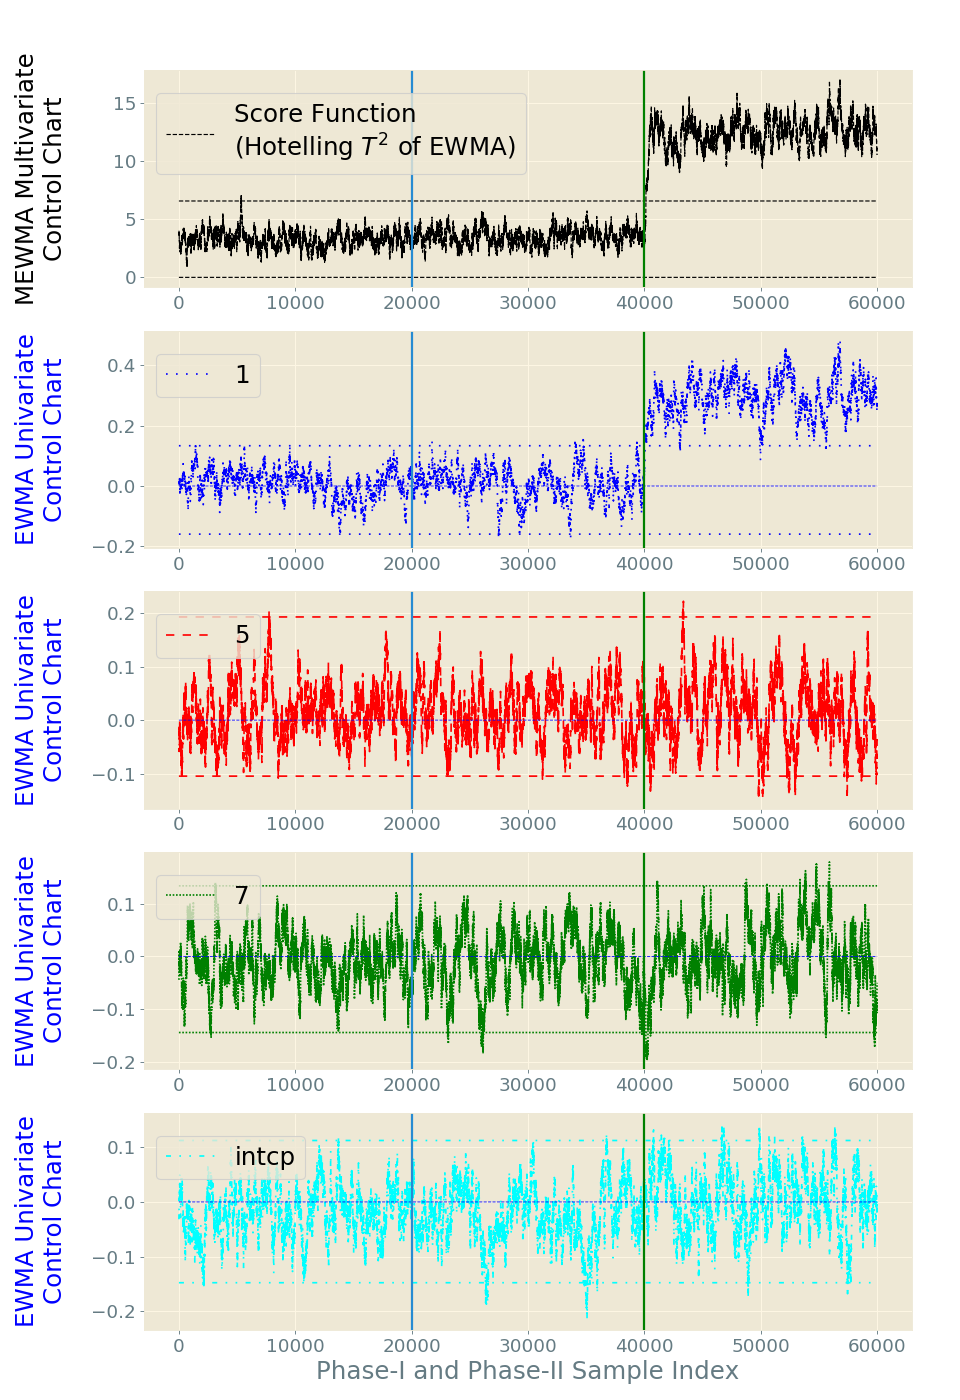
\includegraphics[width = 0.6\linewidth]{../figures/v14/sim_2/reg/neg_single_3_sim2_mlines_with_regu_1e-08_0_005.png}
%  \includegraphics[width = 0.8\linewidth]{../figures/sim_2_pinv_pdf/neg_single_sim2_mlines_with_regu_1e-08_0_005.png}
  \caption{Abrupt concept drift of linear model with independent covariates (colorful in electronic version). For conciseness, here only show EWMA (or MEWMA) control charts for the $1$st (blue), $5$th (red), intercept (green), and Hotelling $T^2$ (black). The blue and green vertical lines mark the boundaries of Phase-I/II and before/after concept drift. The lines of monitored statistics in control charts have the same style and color with lines of their control limits correspondingly.}
  \label{fig:lin_reg_ind_X}
\end{figure}
In this simulation, the dataset is generated by a {linear} model $y = \bm {x}^T\bm { \theta} + \epsilon$. The $10$ {covariates} {$\bm {x}=[x_1, x_2, \cdots, x _{10}]$} are independent Gaussian distributed with mean $0$ and variance $1$; the variance of random error $ \epsilon$ is $1$; the EWMA parameter is $0.027562$ chosen by ensuring around $50\%$ signal ratio after concept drift; there is no penalization in training the model because the number of parameters is small comparing to the sample size; the alarm rate for calculating the control limits is $99.9\%$; the sizes of the dataset used in training, validation, Phase-I, and Phase-II are $10000$, $2000$, $20000$, and $40000$. The responses in training, validation, and Phase-I are generated with coefficients all equal to $1$. In the first half of Phase-II, the coefficients are unchanged, but in the second half, the first four coefficients are multiplied by $1- \alpha=0.7$, where $ \alpha=0.3$ is defined as the changing factor. Other coefficients are unchanged.
\begin{figure}[!htp]
\centering
%   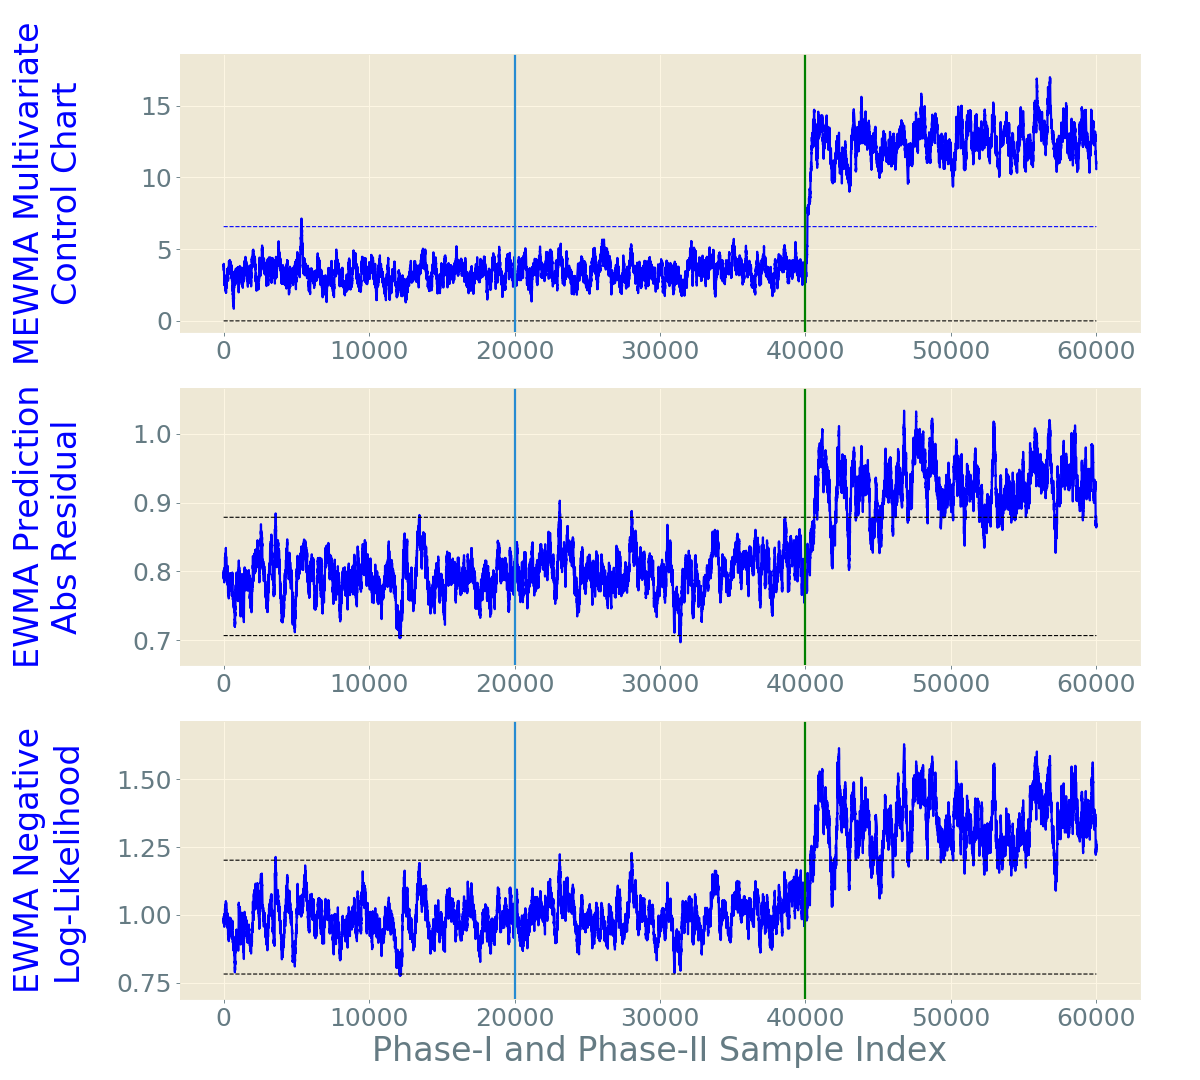
\includegraphics[width = 0.6\linewidth, trim=0in 2.6in 0in 0in, clip]{../figures/v14/sim_2/reg/3_sim2_lin_1e-08_0_005_1.png}
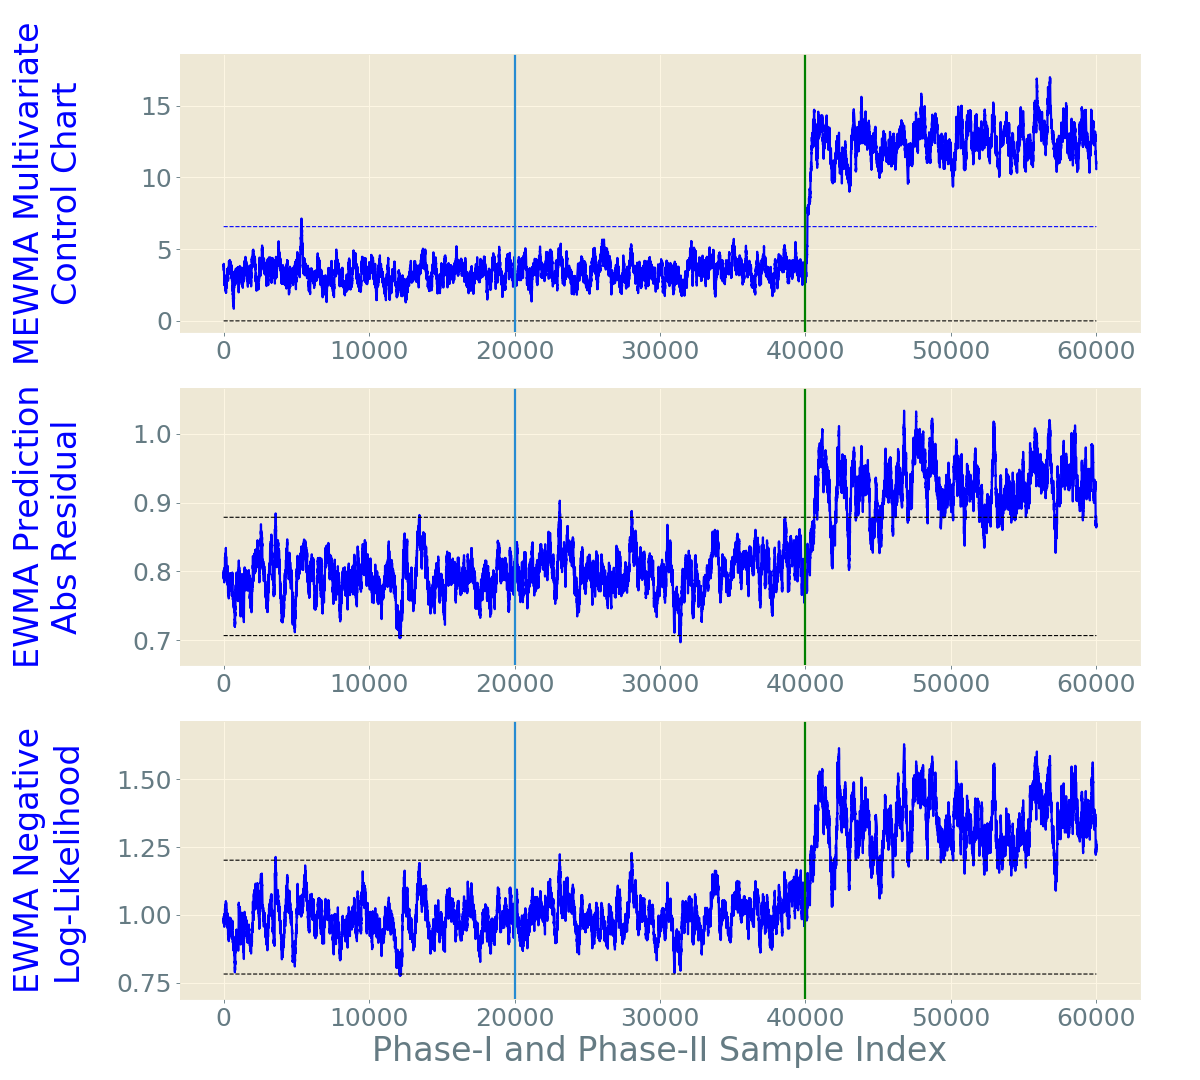
\includegraphics[width = 0.6\linewidth]{../figures/v14/sim_2/reg/3_sim2_lin_1e-08_0_005_1.png}
%  \includegraphics[width = 0.8\linewidth]{../figures/sim_2_pinv_pdf/sim2_ewma_2_metric_with_reg_1e-08_0_005.png}
%  \includegraphics[width = 0.48\linewidth]{../figures/sim_2_pinv/sim2_ewma_log_lik_with_reg_1e-08_0_005.png}
  \caption{Abrupt concept drift of linear model with independent covariates (colorful in electronic version). Control charts of Hotelling $T^2$ of the score function and EWMA of the absolute residual are compared. The lines of monitored statistics in control charts have the same style and color with lines of their control limits correspondingly.}
  \label{fig:lin_reg_ind_X_comp}
\end{figure}

Figure~\ref{fig:lin_reg_ind_X} shows Phase-I and Phase-II of monitoring Hotelling $T^2$ and individual components of the score function. Before blue vertical lines (Phase-I), all lines of monitored statistics are well mixed in their range indicating no concept drift in training and Phase-I. After blue vertical lines (Phase-II), the EWMA lines corresponding to the first four coefficients have significant drifts (only show the first one here) and the change of mean is $0.3$ corresponding to the mean drift of coefficients, contributing to the entire line of MEWMA Hotelling $T^2$ (the black solid line). In this example, all covariates are independent with others, so that there is not coupling, meaning only coefficients with concept drifts would have mean drifts. For brevity, only representative lines are shown. Lines of the rest of coefficients (including intercept) don't have mean drift but have larger deviation after the concept drift, for the reason mentioned in the Section~\ref{ss:var_infla}. The increase of deviation in control charts of those unchanged parameters results from the drifts ($\Delta \bm { \theta}$) coupling with variation of covariates ($X_k\bm {X}^T$).

To compare control charts of Hotelling $T^2$ of the score function and EWMA of the absolute residual, we plot the later two with the one of the score function respectively as shown in Figure~\ref{fig:lin_reg_ind_X_comp}. All of these methods can capture the abrupt concept drift pretty well: in Phase-I they are all mixed well and in Phase-II mean drifts are close to each other. Here, we also see inflated variance of lines after the concept drift, even though they plateau very quickly. The three metrics capture the concept drift quite well, but the score-based method has higher signal ratio after concept drift, indicating that its superior performance in detecting small size changes, which is consistent with the results from the Section~\ref{ss:simu_MRL}. Later, we will show results of the gradual concept drift.

\item
\textbf{Abrupt Concept Drifts with Correlated Covariates}

\label{sss:lin_not_ind_pred}
\begin{figure}[!htbp]
\centering
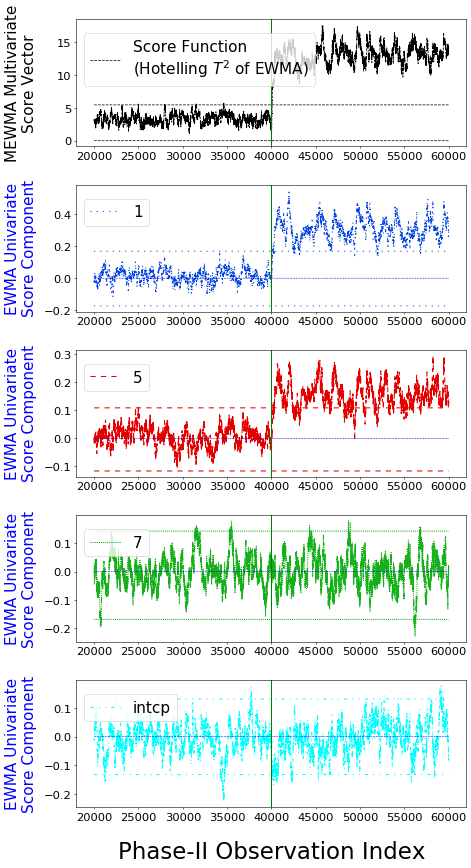
\includegraphics[width = 0.4\linewidth]{../figures/v14/sim_4/reg/PII_neg_single_1_sim4_mlines_with_regu_1e-08_0_005.png}
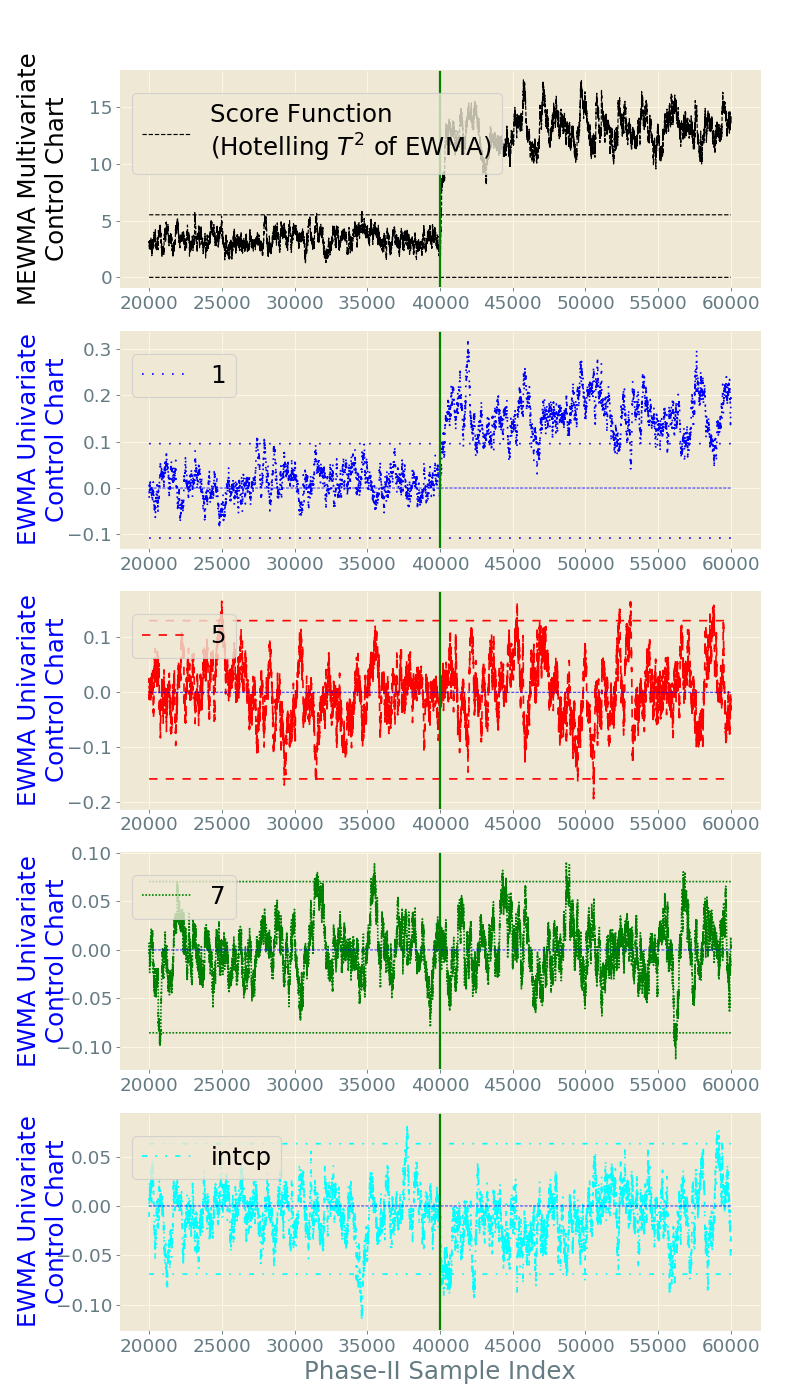
\includegraphics[width = 0.4\linewidth]{../figures/v14/sim_4/reg/PII_neg_single_1_sim4_fisher_mlines_with_regu_1e-08_0_005.png}
%\includegraphics[width = 0.4\linewidth]{../figures/sim_4_1_pinv_pdf/PII_neg_single_sim4_mlines_with_regu_1e-08_0_005.png}
%\includegraphics[width = 0.4\linewidth]{../figures/sim_4_1_pinv_pdf/PII_pos_single_sim4_mlines_fisher_with_regu_1e-08_0_005.png}
%  \includegraphics[width = 1\linewidth]{../figures/sim_3/PII_pos_sim3_mlines_with_regu_1e-08_0_001.png}
%  \includegraphics[width = 1\linewidth]{../figures/sim_3/PII_neg_sim3_mlines_fisher_with_regu_1e-08_0_001.png}
  \caption{Abrupt concept drift of linear model with correlated {covariates} (colorful in electronic version). Comparison are made between before (left) and after (right) being scaled by {the inverse of the estimated} Fisher Information Matrix, {$\mathbf {I} ( {\bm{\theta}} ^{(0)})$.} For legibility, here only show EWMA (or MEWMA) control charts for the $1$st (blue), $5$th (red), $7$th (green), intercept (cyan), and Hotelling $T^2$ (black). The lines of monitored statistics in control charts have the same style and color with lines of their control limits correspondingly.}
  \label{fig:lin_reg_not_ind_X}
\end{figure}
Then, we manually introduce correlation between {covariates} by setting $0.5 x_1 + 0.5 x_5$ and $ 0.3 x_1 + 0.3 x_2 + 0.4 x_6$ as new $x_5$ and $x_6$ respectively, with others remaining the same. The EWMA and MEWMA control charts before (left) and after (right) scaled by {the inverse of the estimated} ${\mathbf {I}}(\bm { \theta}^{(0)})$ is as shown in Figure~\ref{fig:lin_reg_not_ind_X}. The blue and red lines are for $x_1$ and $x_7$: scaling or not has no effect on those lines, where the coefficient for $x_1$ has mean {drift} but $x_7$ doesn't. However, according to the green line for $x_5$, scaling changes it from having mean {drift} to not, indicating that this scaling successfully decouples concept drift from correlated covariates. This is not surprising, because ${\mathbf {I}} ^{-1}(\bm { \theta}^{(0)})$ equals to $E ^{-1} [\bm {X}\bm {X}^T]$, which doesn't depend on $ \bm { \theta} ^{(0)}$ or $ \bm { \theta} ^{(1)}$, meaning high-ordered term in equation (\ref{eqn:fisher_approx}) is zero. However, in the next experiment for logistic regression, the concept drift is harder to decouple because multiplying ${\mathbf {I}} ^{-1}(\bm { \theta}^{(0)})$ can only approximately decouple concept drifts.

\item
\textbf{Gradual Concept Drifts with Correlated Covariates}
\label{sss:lin_not_ind_pred_grad_cd}
\begin{figure}[!htbp]
\centering
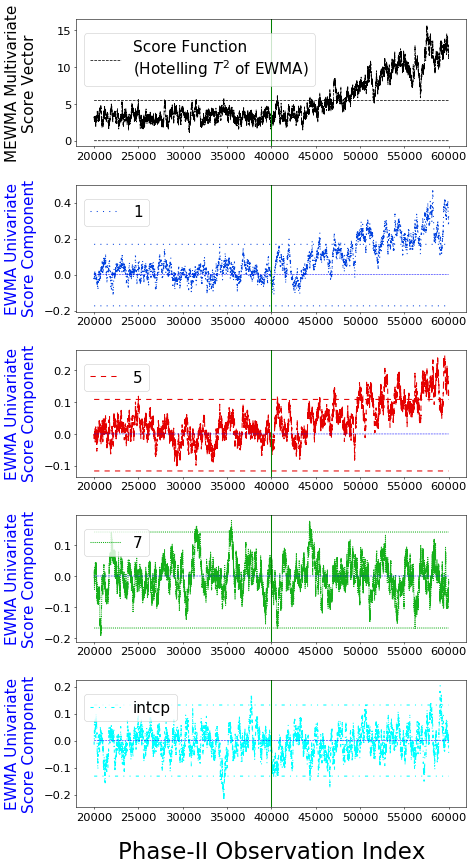
\includegraphics[width = 0.4\linewidth]{../figures/v14/sim_6/reg/PII_neg_single_1_sim6_mlines_with_regu_1e-08_0_005.png}
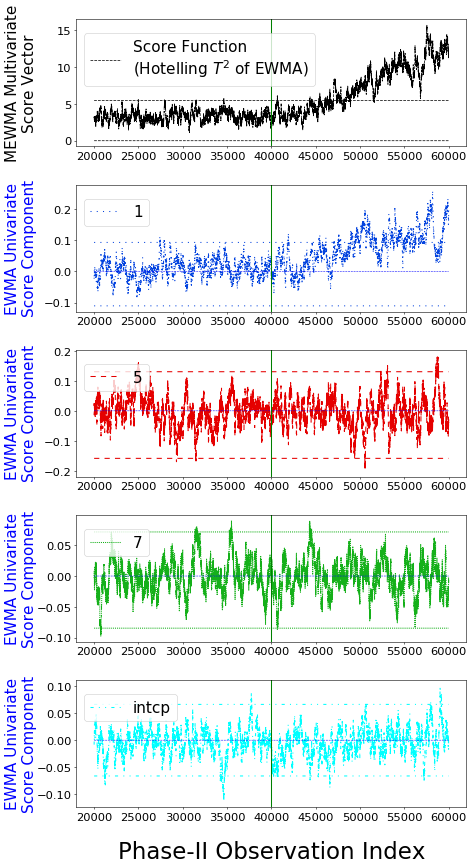
\includegraphics[width = 0.4\linewidth]{../figures/v14/sim_6/reg/PII_neg_single_1_sim6_fisher_mlines_with_regu_1e-08_0_005.png}
%\includegraphics[width = 0.4\linewidth]{../figures/sim_6_1_pinv_pdf/PII_neg_single_sim6_mlines_with_regu_1e-08_0_005.png}
%\includegraphics[width = 0.4\linewidth]{../figures/sim_6_1_pinv_pdf/PII_pos_single_sim6_mlines_fisher_with_regu_1e-08_0_005.png}
 \caption{Gradual concept drift of linear model with correlated {covariates} (colorful in electronic version). Comparison are made between before (left) and after (right) being scaled by {the inverse of the estimated} Fisher Information Matrix, {$\mathbf {I} ( {\bm{\theta}} ^{(0)})$.} For legibility, here only show EWMA (or MEWMA) control charts for the $1$st (blue), $5$th (red), $7$th (green), intercept (cyan), and Hotelling $T^2$ (black). The left (right) vertical axis is for univariate (multivariate) control charts. The lines of monitored statistics in control charts have the same style and color with lines of their control limits correspondingly.}
  \label{fig:lin_reg_not_ind_X_grad_cd}
\end{figure}
In real applications, many concept drifts happen in a gradual way. In this dataset, all conditions are the same with that in the Section~\ref{sss:lin_not_ind_pred} except that the concept drifts happen linearly in the second half time of Phase-II. The starting and ending coefficients of the linear concept drift period correspond to those before and after concept drifts in the abrupt case. 
\begin{figure}[!htbp]
\centering
% \includegraphics[width = 0.48\linewidth]{../figures/sim_6_1_pinv_pdf/sim6_ewma_resi_with_reg_1e-08_0_005.png}
%\includegraphics[width = 0.8\linewidth]{../figures/sim_6_1_pinv_pdf/sim6_ewma_2_metric_with_reg_1e-08_0_005.png}
% 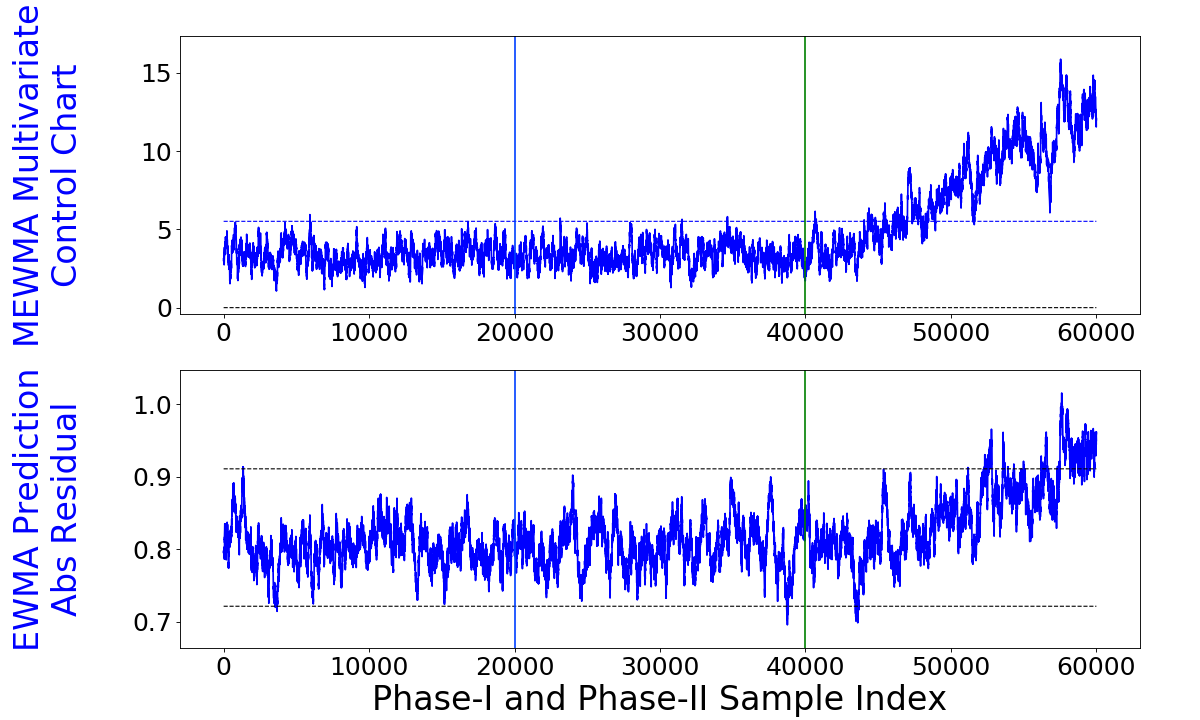
\includegraphics[width = 0.6\linewidth, trim=0in 2.6in 0in 0in, clip]{../figures/v14/sim_6/reg/1_sim6_lin_1e-08_0_005_1.png}
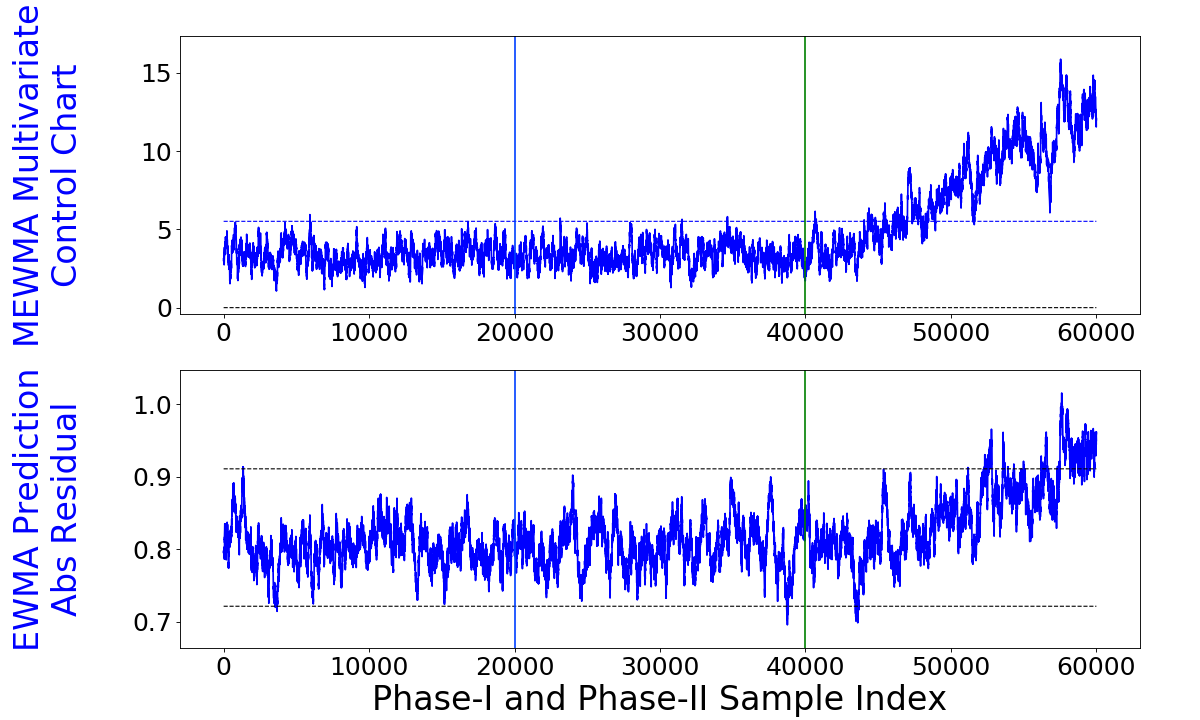
\includegraphics[width = 0.6\linewidth]{../figures/v14/sim_6/reg/1_sim6_lin_1e-08_0_005_1.png}
  \caption{Gradual concept drift of linear model with correlated covariates (colorful in electronic version). Control charts of Hotelling $T^2$ of the score function and EWMA of the absolute residual are compared. The lines of monitored statistics in control charts have the same style and color with lines of their control limits correspondingly.}
  \label{fig:lin_reg_ind_X_grad_cd_comp}
\end{figure}

The EWMA and MEWMA control charts before (left) and after (right) scaled by {the inverse of the estimated} ${\mathbf {I}}(\bm { \theta}^{(0)})$ is as shown in Figure~\ref{fig:lin_reg_not_ind_X_grad_cd}. Similarly with that in the Section~\ref{sss:lin_not_ind_pred}, lines corresponding to covariates with true concept drifts or independent with others are not affected by scaling in terms whether concept drifts show up in control charts. In Figure~\ref{fig:lin_reg_ind_X_grad_cd_comp}, we see that monitoring the score vectors gives an earlier detection of the starting position of the concept drift than EWMA of the absolute residual.
\end{enumerate}

\subsubsection{Simulated Dataset for Logistic Regression}
\begin{enumerate}[(I)]
\item
\textbf{Abrupt Concept Drifts with Independent Covariates}
\label{sss:log_ind_pred}
\begin{figure}[!htbp]
\centering
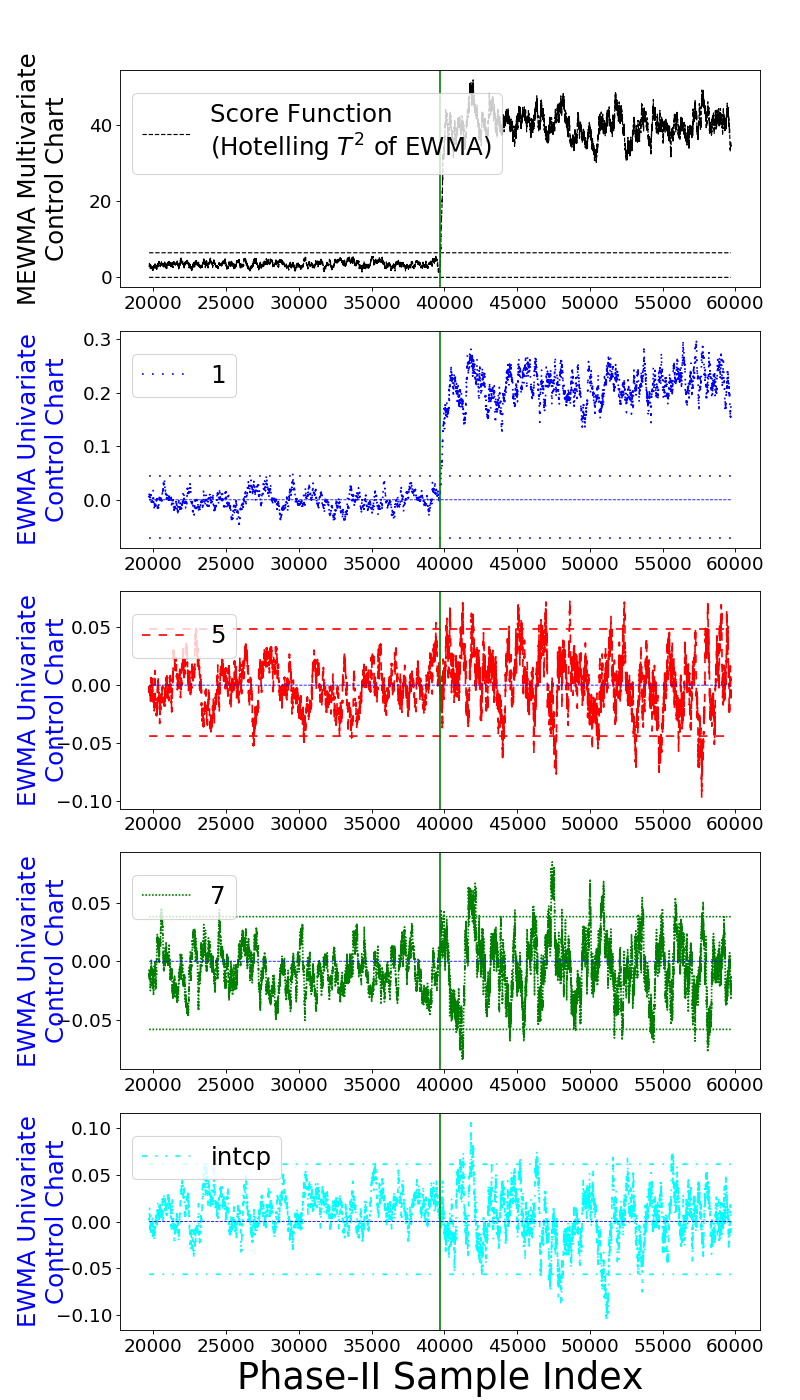
\includegraphics[width = 0.4\linewidth]{../figures/v14/sim_5/logi_no_muco/PII_pos_single_1_sim5_mlines_with_regu_1e-08_0_005.png}
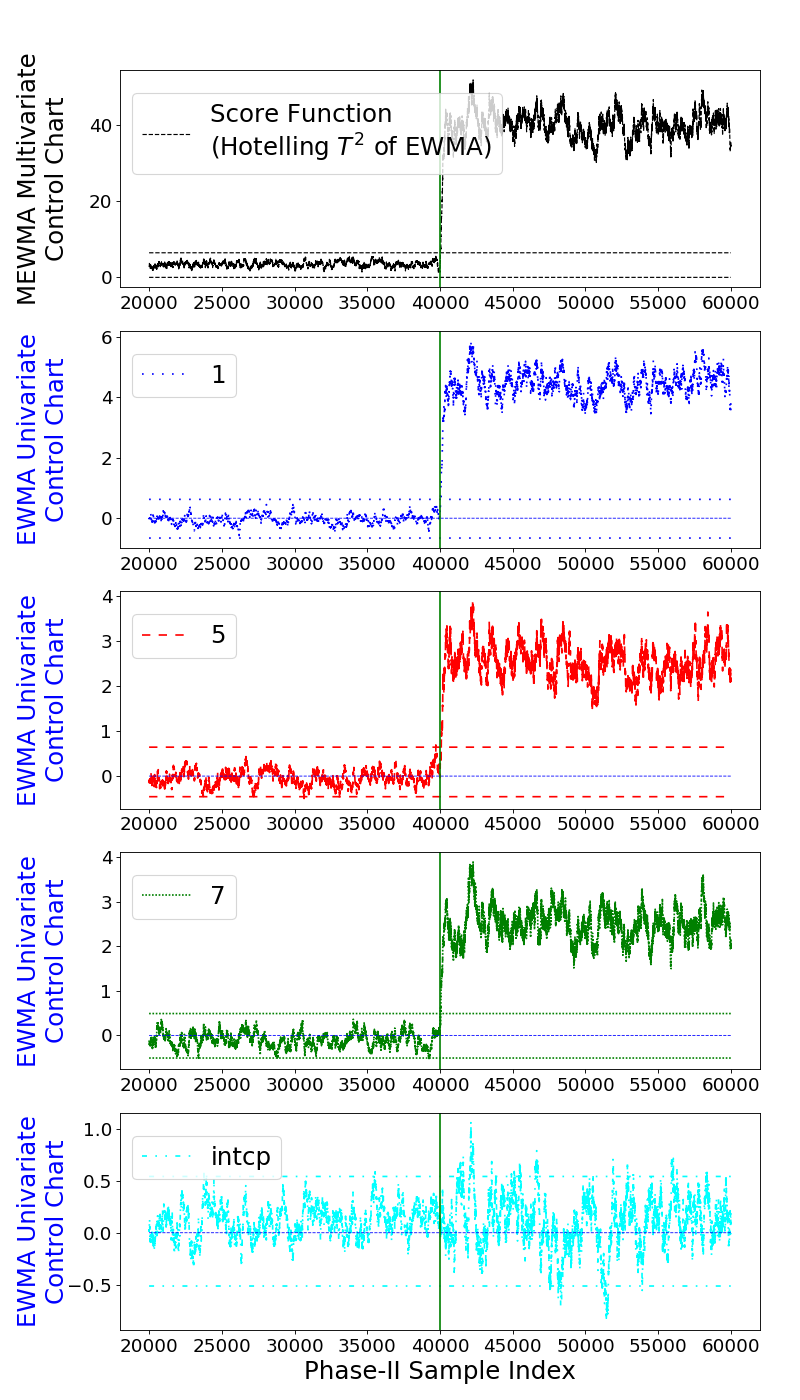
\includegraphics[width = 0.4\linewidth]{../figures/v14/sim_5/logi_no_muco/PII_pos_single_1_sim5_fisher_mlines_with_regu_1e-08_0_005.png}
%\includegraphics[width = 0.4\linewidth]{../figures/sim_3_pinv_pdf/PII_pos_single_sim3_mlines_with_regu_1e-08_0_005.png}
%\includegraphics[width = 0.4\linewidth]{../figures/sim_3_pinv_pdf/PII_neg_single_sim3_mlines_fisher_with_regu_1e-08_0_005.png}
%  \includegraphics[width = 1\linewidth]{../figures/sim_3/PII_pos_sim3_mlines_with_regu_1e-08_0_001.png}
%  \includegraphics[width = 1\linewidth]{../figures/sim_3/PII_neg_sim3_mlines_fisher_with_regu_1e-08_0_001.png}
  \caption{Abrupt concept drift of logistic regression with independent {covariates} (colorful in electronic version). Comparison are made between before (left) and after (right) being scaled by {the inverse of the estimated} Fisher Information Matrix, {$\mathbf {I} ( {\bm{\theta}} ^{(0)})$.} For legibility, here only show EWMA (or MEWMA) control charts for the $1$st (blue), $5$th (red), $7$th (green), intercept (cyan), and Hotelling $T^2$ (black). The lines of monitored statistics in control charts have the same style and color with lines of their control limits correspondingly.}
  \label{fig:log_reg_ind_X}
\end{figure}

This simulated dataset has the same parameter as that in the corresponding Section~\ref{sss:lin_ind_pred}, except that here the model becomes {logistic model} {$p(y=1|\bm {x})= \sigma (\bm {x}^T\bm { \theta})$,} where $\sigma (\cdot)$ is the sigmoid function.
\begin{figure}[!htbp]
\centering
% 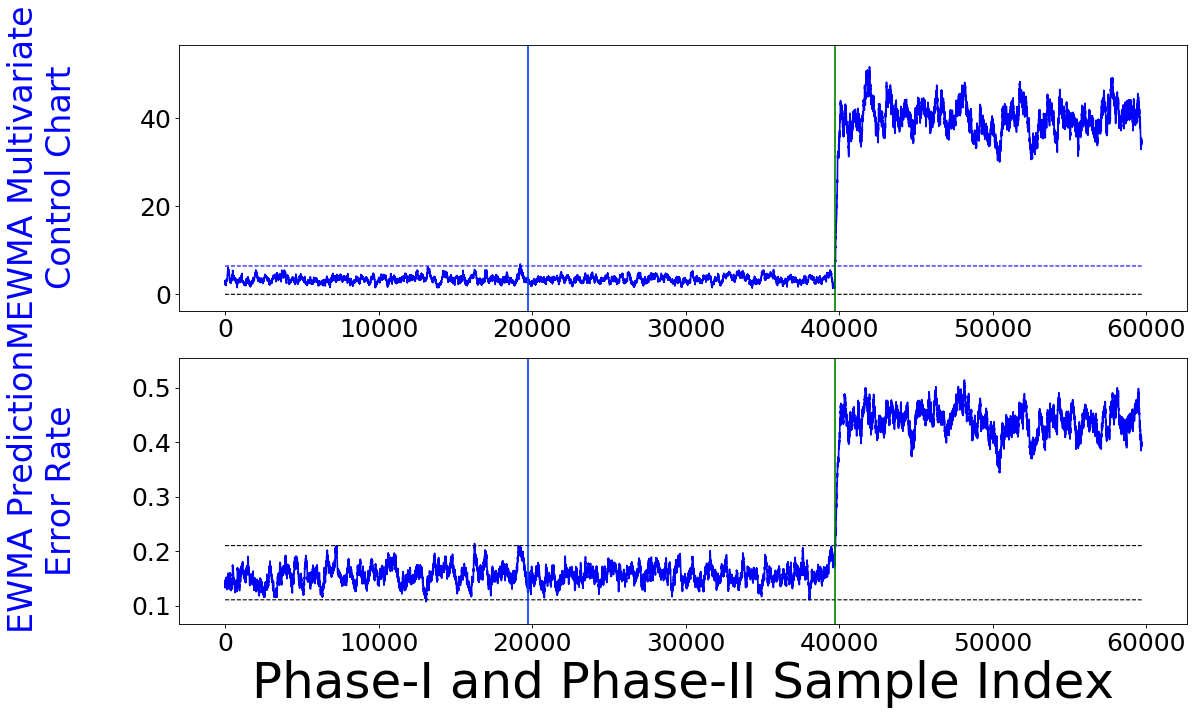
\includegraphics[width = 0.6\linewidth, trim=0in 2.6in 0in 0in, clip]{../figures/v14/sim_5/logi_no_muco/1_sim5_logi_1e-08_0_005_1.png}
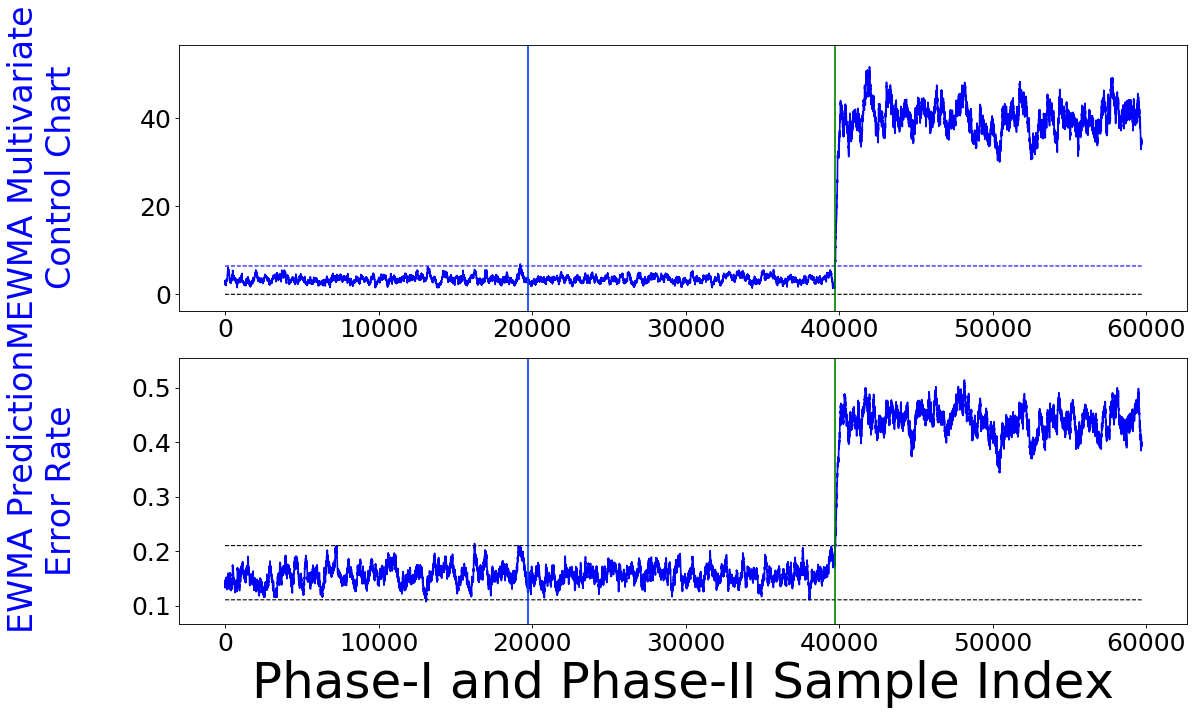
\includegraphics[width = 0.6\linewidth]{../figures/v14/sim_5/logi_no_muco/1_sim5_logi_1e-08_0_005_1.png}
%  \includegraphics[width = 0.49\linewidth]{../figures/sim_3_pinv_pdf/sim3_ewma_2_metric_with_reg_1e-08_0_005.png}
%  \includegraphics[width = 0.49\linewidth]{../figures/sim_3_pinv_pdf/sim3_ewma_2_metric_with_reg_1e-08_0_002.png}
%  \includegraphics[width = 0.24\linewidth]{../figures/sim_3_pinv_pdf/sim3_ewma_dev_with_reg_1e-08_0_005.png}
%  \includegraphics[width = 0.24\linewidth]{../figures/sim_3_pinv_pdf/sim3_ewma_dev_with_reg_1e-08_0_001.png}
  \caption{Abrupt concept drift of logistic regression with independent covariates (colorful in electronic version). Control charts of Hotelling $T^2$ of the score function and EWMA of the error rate are compared. The lines of monitored statistics in control charts have the same style and color with lines of their control limits correspondingly.}
  \label{fig:log_reg_ind_X_comp}
\end{figure}

As shown in Figure~\ref{fig:log_reg_ind_X}, even though components of $\bm {x}$ are independent, the concept drifts of the first four components still propagate to the rest (with smaller magnitude) which don't have drifts, except the intercept (because of the symmetry of distribution of our simulated $\bm {x}$). This is because $E [ (\sigma ( \bm {X}^T\bm { \theta}^{(1)} ) - \sigma ( \bm {X}^T\bm { \theta}^{(0)} )) \bm {X}] $ has a nonlinear term and depends on parameters. This is supported by the comparison of the left and right column in Figure~\ref{fig:log_reg_ind_X}: applying scaling matrix cannot recover zero mean drift for those covariates without concept drift (the red line for $x_5$) meaning this coupling is due to the nonlinearity rather than correlation between covariates. During experiments, we find an interesting special case that if the concept drift is restricted to flipping sign of coefficients, the covariates without concept drift will not have mean {drift} (no coupling effect) in those control charts, due to the same reason that the intercept has no mean drift.

As the comparison in the Section~\ref{sss:lin_ind_pred}, in Figure~\ref{fig:log_reg_ind_X_comp}, control charts of Hotelling $T^2$ of the score function and EWMA of the prediction error, both methods can capture the abrupt concept drift, but the EWMA of the prediction error has much less signal ratio. This is because in Phase-I the prediction error has a wider range between control limits than that of the score function, so that in Phase-II the control chart is less sensitive to the deviation.

\item
\textbf{Abrupt Concept Drifts with Correlated Covariates}
\label{sss:log_not_ind_pred}
\begin{figure}[!htbp]
\centering
\includegraphics[width = 0.4\linewidth]{../figures/v14/sim_5/logi/PII_pos_single_1_sim5_mlines_with_regu_1e-08_0_005.png}
\includegraphics[width = 0.4\linewidth]{../figures/v14/sim_5/logi/PII_pos_single_1_sim5_fisher_mlines_with_regu_1e-08_0_005.png}
%  \includegraphics[width = 0.4\linewidth]{../figures/sim_3_1_pinv_pdf/PII_pos_single_sim3_mlines_with_regu_1e-08_0_005.png}
%  \includegraphics[width = 0.4\linewidth]{../figures/sim_3_1_pinv_pdf/PII_neg_single_sim3_mlines_fisher_with_regu_1e-08_0_005.png}
  \caption{
Abrupt concept drift of logistic regression with correlated {covariates} (colorful in electronic version). Comparison are made between before (left) and after (right) being scaled by {the inverse of the estimated} Fisher Information Matrix, {$\mathbf {I} ( {\bm{\theta}} ^{(0)})$.} For legibility, here only show EWMA (or MEWMA) control charts for the $1$st (blue), $5$th (red), $7$th (green), intercept (cyan), and Hotelling $T^2$ (black). The lines of monitored statistics in control charts have the same style and color with lines of their control limits correspondingly.
% Concept drift of logistic regression with correlated {covariates} (colorful in electronic version). Comparison are made between before (above) and after (below) being scaled by {the inverse of the estimated} Fisher Information Matrix, {$\mathbf {I} ( {\bm{\theta}} ^{(0)})$.} 
}
  \label{fig:log_reg_not_ind_X}
\end{figure}
As in the Section~\ref{sss:lin_not_ind_pred}, we introduce correlation between {covariates.} The comparison between before and after scaling with {the inverse of the estimated} {$\mathbf {I} ( {\bm{\theta}} ^{ (0)}) = E [{p} (\bm {X},\bm { \theta} ^{ (0)}) (1-{p}(\bm {X},\bm { \theta} ^{ (0)})) \bm {X} \bm {X}^T] \Delta \bm{ \theta}$}, where {$p (\bm {X},\bm { \theta} ^{ (0)}) = \sigma ( \bm {X}^T\bm { \theta} ^{ (0)})$}, is shown in Figure~\ref{fig:log_reg_not_ind_X}. The scaling makes the mean {drift} uniformly significant on control charts over all {covariates,} no matter whether they have concept drift (here only show representative lines). For the $x_7$ (green) component, previously mild concept drift due to nonlinearity becomes even larger (worse) after scaling. This indicates that the approximation in equation (\ref{eqn:fisher_approx}) is not accurate. This makes sense, because the concept drift is large (coefficients from $1$ to $-1$), violating the assumption of ``small higher-ordered terms of concept drift". 

\item
\textbf{Concept Drifts with Correlated Covariates and an Assumption}
\label{sss:log_not_ind_pred_assum}
\begin{figure}[!htbp]
\centering
\includegraphics[width = 0.4\linewidth]{../figures/v14/sim_5/logi_small/PII_pos_single_1_sim5_mlines_with_regu_1e-08_0_005.png}
\includegraphics[width = 0.4\linewidth]{../figures/v14/sim_5/logi_small/PII_pos_single_1_sim5_fisher_mlines_with_regu_1e-08_0_005.png}
%  \includegraphics[width = 0.4\linewidth]{../figures/sim_5_1_pinv_pdf/PII_pos_single_sim5_mlines_with_regu_1e-08_0_005.png}
%  \includegraphics[width = 0.4\linewidth]{../figures/sim_5_1_pinv_pdf/PII_neg_single_sim5_mlines_fisher_with_regu_1e-08_0_005.png}
  \caption{
 Abrupt concept drift of logistic regression with correlated covariates (colorful in electronic version). Simulated data are modified to reduce the magnitude of $ \bm {x}_i^T\bm { \theta}^{(1)}$ and $  \bm {x}_i^T\bm { \theta}^{(0)}$. Comparison are made between before (left) and after (right) being scaled by the inverse of the estimated Fisher Information Matrix, $\mathbf {I} ( {\bm{\theta}} ^{(0)})$. For legibility, here only show EWMA (or MEWMA) control charts for the $1$st (blue), $5$th (red), $7$th (green), intercept (cyan), and Hotelling $T^2$ (black). The lines of monitored statistics in control charts have the same style and color with lines of their control limits correspondingly.
%Concept drift of logistic regression with correlated covariates.  Simulated data are modified to reduce the magnitude of $ \bm {x}_i^T\bm { \theta}^{ (1)}$ and $  \bm {x}_i^T\bm { \theta}^{ (0)}$. Comparison are made between before (above) and after (below) being scaled by the inverse of the estimated Fisher Information Matrix, $\mathbf {I} ( {\bm{\theta}} ^{(0)})$. 
}
  \label{fig:log_reg_not_ind_X_1}
\end{figure}

To resolve the failure of diagnosing true concept drifts in \ref{sss:log_not_ind_pred}, we observe that, according to the mean drift of logistic regression $E [ (\sigma (\bm {X}^T\bm { \theta}^{ (1)}) - \sigma ( \bm {X}^T\bm { \theta}^{ (0)})) \bm {X}] $, if $ \bm {x}^T\bm { \theta}^{ (1)}$ and $ \bm {x}^T\bm { \theta}^{ (0)}$ are all relative small (say $\ll 4$ in absolute value), the sigmoid function $ \sigma (\cdot)$ are in the linear region, so that we can approximate the mean drift by $E [ (\sigma ( \bm {X}^T\bm { \theta}^{ (1)} ) - \sigma ( \bm {X}^T\bm { \theta}^{ (0)} )) \bm {X}] \approx E [ \alpha( \bm {X}^T\bm { \theta}^{ (1)} -  \bm {X}^T\bm { \theta}^{ (0)} ) \bm {X}] = \alpha E[\bm{XX}^T] \Delta \bm { \theta} $, where $ \alpha$ is just a scalar constant factor, reducing to the case of linear model.  

To test this argument, we follow the dataset generating process in the Section~\ref{sss:log_not_ind_pred} but make modifications as below: the coefficients of all covariates in training, validation, Phase-I, and the first half period of Phase-II changes to $0.2$; in the second half period of Phase-II, the coefficients of the first four covariates are multiplied by $-1$. In Figure~\ref{fig:log_reg_not_ind_X_1}, we observe that, scaling or not doesn't change the lines corresponding to covariates which are independent with others or truly have concept drifts in terms of whether show concept drifts in control charts (the coefficient for $x_1$ (blue) has mean drift but $x_7$ (green) and intercept (cyan) doesn't); but scaling changes the line $x_5$ (red) in the control charts from having mean drift to not. In other words, the concept drifts are successfully decoupled. Due to the reduced variance of covariates and smaller concept drifts, the variance inflation after concept drifts is also mitigated, as shown in the second half of Phase-II. Even though this requires some assumption, this property of logistic regression is still practically valuable, because when arguments of sigmoid function have large absolute value, large concept drifts may not have much impact on the performance of predictive models (the sigmoid function is in the plateau regions), while when the sigmoid function is in linear region, small drifts in coefficients can significantly change prediction, so that we might want to understand which covariates contribute to such change. 

This property of logistic regression can be extended to gradual concept drifts. Modifying the above dataset as in the section \ref{sss:lin_not_ind_pred_grad_cd}, meaning change the abrupt concept drift to linear one.
\begin{figure}[!htbp]
\centering
\includegraphics[width = 0.4\linewidth]{../figures/v14/sim_7/logi_small/PII_pos_single_1_sim7_mlines_with_regu_1e-08_0_005.png}
\includegraphics[width = 0.4\linewidth]{../figures/v14/sim_7/logi_small/PII_pos_single_1_sim7_fisher_mlines_with_regu_1e-08_0_005.png}
%\includegraphics[width = 0.4\linewidth]{../figures/sim_7_1_pinv_pdf/PII_pos_single_sim7_mlines_with_regu_1e-08_0_005.png}
%\includegraphics[width = 0.4\linewidth]{../figures/sim_7_1_pinv_pdf/PII_neg_single_sim7_mlines_fisher_with_regu_1e-08_0_005.png}
 \caption{Gradual concept drift of logistic regression with correlated {covariates} (colorful in electronic version). Comparison are made between before (left) and after (right) being scaled by {the inverse of the estimated} Fisher Information Matrix, {$\mathbf {I} ( {\bm{\theta}} ^{(0)})$.} For legibility, here only show EWMA (or MEWMA) control charts for the $1$st (blue), $5$th (red), $7$th (green), intercept (cyan), and Hotelling $T^2$ (black). The left (right) vertical axis is for univariate (multivariate) control charts. The lines of monitored statistics in control charts have the same style and color with lines of their control limits correspondingly.}
  \label{fig:log_reg_not_ind_X_grad_cd}
\end{figure}
\begin{figure}[!htbp]
\centering
% \includegraphics[width = 0.6\linewidth, trim=0in 2.6in 0in 0in, clip]{../figures/v14/sim_7/logi_small/1_sim7_logi_1e-08_0_005_1.png}
\includegraphics[width = 0.6\linewidth]{../figures/v14/sim_7/logi_small/1_sim7_logi_1e-08_0_005_1.png}
% \includegraphics[width = 0.8\linewidth]{../figures/sim_7_1_pinv_pdf/sim7_ewma_2_metric_with_reg_1e-08_0_005.png}
%\includegraphics[width = 0.48\linewidth]{../figures/sim_7_1_pinv_pdf/sim7_ewma_dev_with_reg_1e-08_0_005.png}
  \caption{Gradual concept drift of logistic regression with correlated covariates (colorful in electronic version). Control charts of Hotelling $T^2$ of the score function and EWMA of the absolute residual are compared. The lines of monitored statistics in control charts have the same style and color with lines of their control limits correspondingly.}
  \label{fig:log_reg_ind_X_grad_cd_comp}
\end{figure}

The EWMA and MEWMA control charts before (left) and after (right) scaled by {the inverse of the estimated} ${\mathbf {I}}(\bm { \theta}^{(0)})$ is as shown in Figure~\ref{fig:log_reg_not_ind_X_grad_cd}. Similarly with that in Figure \ref{fig:log_reg_not_ind_X_1}, lines corresponding to covariates with true concept drifts or independent with others are not affected by scaling in terms whether show concept drifts in figures, confirming the validity of the assumption in this section. In Figure~\ref{fig:log_reg_ind_X_grad_cd_comp}, we see that monitoring the score vectors renders an even much earlier detection of the starting position of the concept drift than EWMA of the prediction error rate.

In summary, we demonstrated the efficacy of using MEWMA control charts to monitor the score function in detecting concept drifts. And we also show how to diagnose the concept drifts by applying proper scaling and EWMA control charts. Also, we discussed the coupling due to multicollinearity and nonlinearity and how to resolve those issues. The practicability of the assumption of small argument for decoupling concept drifts in logistical regression was also justified. Next, this method will be considered and used in two real datasets.
\end{enumerate}

\section{Real Datasets}
The concept drifts is usually hard to directly testify in real life, because the existence of concept drift results from some hidden effects or contexts which models don't incorporate. If such hidden effects or contexts are founded and can be quantified, it becomes a different problem because they can be included into the model to increase predictability. However, there are some events having generally accepted prior or posterior that can be used as evidence of concept drifts. For example, $2008$ economic crash is a big context change for financial industry. Another one is the recently boosting of ``sharing economy", like bike sharing. Even though none of the two examples satisfies the definition of ``abrupt concept drift", the first example evolves much faster than the second one. So in comparison, we can think the first example is closer to an ``abrupt concept drift" and the second one is closer to a ``gradual concept drift". In this section, we will apply the monitoring and diagnosis procedures mentioned above to two real datasets, and provide a real case study in how these methods can improve our understanding or model performance.

\subsection{Credit Risk Dataset}
\label{ss:cr_ds}
\begin{figure}[!htbp]
\centering
%  \includegraphics[width = 0.49\linewidth]{../figures/v14/credit_default/lin_model_pinv_pdf/credit_ewma_2_metric_with_reg_21_544346128_0_001.png}
	\includegraphics[width = 0.49\linewidth, trim=0in 2.6in 0in 0in, clip]{../figures/v14/credit_default/logi_scal_train_PI/credit_logi_1e-08_0_0001_0_001_99_0.png}
%    \includegraphics[width = 0.24\linewidth]{../figures/v14/credit_default/lin_model_pinv_pdf/credit_ewma_dev_with_reg_21_544346128_0_001.png}
%    \includegraphics[width = 0.49\linewidth]{../figures/v14/credit_default/nnet_model_pinv_pdf/credit_ewma_2_metric_with_reg_0_001_0_001.png}
\includegraphics[width = 0.49\linewidth, trim=0in 2.6in 0in 0in, clip]{../figures/v14/credit_default/logi_nnet_scal_train_PI/credit_logi_0_001_0_0001_0_001_99_0.png}
%     \includegraphics[width = 0.24\linewidth]{../figures/v14/credit_default/nnet_model_pinv_pdf/credit_ewma_dev_with_reg_0_001_0_001.png}    
  \caption{
Control charts monitoring MEWMA of Hotelling $T^2$ of the score function and EWMA of the prediction error are compared using credit risk dataset. The left plots are from logistic regression, and the right from MLP with one hidden layer of $50$ nodes. The tilted numbers along the x-axis, as the indices of month, are the time of credit card defaults. For example, $601$ stands for 2006-Jan. So the index $712$ is for the 2007-Dec, right after which a $15$-month significant drop began (S\&P 500 from $1478.49$ on 2007-Dec.28 to $683.38$ on 2009-Mar.28).
%MEWMA of Hotelling $T^2$ control charts are used to monitor the concept drift of credit risk dataset. The above two plots are from logistic regression, and the below from neural network with one hidden layer of $50$ nodes. The left and the right vertical axis is for control chart and cumulative prediction accuracy. The tilted numbers along the x-axis, as the indices of month, are the time at openings of credit card accounts. For example, $601$ stands for Jan.06. So the index $712$ is for the Dec.07, right after which a $15$-month significant drop began (S\&P 500 from $1478.49$ on Dec.28,07 to $735.09$ on Feb.28,08).
}
\label{fig:credit_default}
\end{figure}
The credit risk dataset contains customer information (features, centered covariates,  $\bm {x}_i$) of credit card applications to a major financial company and labels indicating whether customers default within $9$-month after opening the account (response, $y_i$). The data is originally used in~(\cite{im2012time}) where $10$ statistically significant covariates are selected based on a forward feature selection method. Here, we inherit the processed dataset and covariates, which will not be specifically described, due to confidentiality concerns. Then, a logistic regression model and classification MLP (one hidden layer with $50$ hidden nodes) are trained and validated on around half of data starting from 2003-Jan to 2005-Dec (monthly indexed from $301$ to $512$). Data from 2006-Jan to 2006-Dec are used in Phase-I to calculate control limits and the rest of data until 2008-Aug are used for Phase-II to test the capability of detecting the concept drift due to economic crisis. Because the noise is very large in this dataset, we choose $ \lambda = 0.001$ as EWMA parameter.

The underlying concept drift for predictive models trained on covariates (prepared by the financial company) and responses can be resulted from many hidden effects. The overall economic crisis is probably one of major reasons and we can use this to test the efficacy of our model. 

Figure~\ref{fig:credit_default} consists of Phase-I and Phase-II MEWMA Hotelling $T^2$ of the score function for logistic regression and MLP. We also compare our method with EWMA of the prediction error, state-of-art metrics among many current concept drift detection methods~(\cite{barros2018large}). From Phase-II control charts, the increasing trend starts around the index $702$, which stands for 2007-Feb. This time plus $9$-month is close to the breakout of then economic crisis, featured by the beginning of a $15$-month falling of S\&P 500 index by more than $50\%$. Even though the monitoring statistics are almost all in-control before 2007-Jul, they are consistently near the upper control limit with increasing trend. This suggests the drift might start even a few months earlier, which is reasonable because the economic crisis was unlikely to happen in a sudden way. Both logistic regression and MLP work well in terms of early detecting the concept drift, suggesting that our method is compatible with models which have a large number of parameters. From EWMA of the prediction error, the detection points are later than that of monitoring the score function. The overall pattern of our control charts indicates that using control chart to monitor the score function leads to early detection of concept drift. 

\begin{figure}[!htbp]
\centering
%  \includegraphics[width = 0.48\linewidth]{../figures/v14/credit_default/lin_model_pinv_pdf/PII_pos_single_credit_mlines_with_regu_21_544346128_0_001.png}
%  \includegraphics[width = 0.48\linewidth]{../figures/v14/credit_default/lin_model_pinv_pdf/PII_neg_single_credit_mlines_fisher_with_regu_21_544346128_0_001.png}
 \includegraphics[width = 0.48\linewidth]{../figures/v14/credit_default/logi_scal_train_PI/PII_pos_single_credit_mlines_with_regu_1e-08_0_0001_0_001_99_0.png}
  \includegraphics[width = 0.48\linewidth]{../figures/v14/credit_default/logi_scal_train_PI/PII_pos_single_credit_fisher_mlines_with_regu_1e-08_0_0001_0_001_99_0.png}
  \caption{
  MEWMA and EWMA control charts for logistic regression of credit risk dataset (colorful in electronic version). Comparison are made between before (left) and after (right) being scaled by the inverse of the estimated Fisher Information Matrix, $\mathbf {I} ( {\bm{\theta}} ^{(0)})$. For legibility, here only show EWMA (or MEWMA) control charts for the $1$st (blue), $2$nd (red), $3$rd (green), $8$th (cyan), intercept (orange), and Hotelling $T^2$ (black). The lines of monitored statistics in control charts have the same style and color with lines of their control limits correspondingly.
%MEWMA and EWMA control charts for logistic regression of credit risk dataset. Comparison are made between before (above) and after (below) being scaled by the inverse of the estimated Fisher Information Matrix, $\mathbf {I} ( {\bm{\theta}} ^{(0)})$. 
}
\label{fig:credit_default_diag}
\end{figure}

To demonstrate the diagnostic functionality on this real dataset, EWMA of sample score vectors of the logistic regression model for several covariates are compared before and after scaling with the the inverse of the estimated Fisher Information Matrix, $\mathbf {I} ( {\bm{\theta}} ^{(0)})$. In Figure~\ref{fig:credit_default_diag}, EWMA of sample score vectors of several representative scalar covariates are plotted before and after scaling. The MEWMA Hotelling $T^2$ (black solid) are also put at the top row for the ease of comparison, even though the scaling has no effect on it. As shown, the $1$st (blue) and $2$nd (red) covariates have significant mean drift before scaling, but mean drift of the $2$nd predictor is largely shrunk to zero after scaling. Those two covariates has $0.45$ correlation, and the $2$nd one has more general thus less direct impact than the $1$st on the credit risk assessment. Thus it is reasonable to think that the concept drift is more likely due to the change of effect of the $1$st predictor instead of that of the $2$nd. Lines of the $3$rd (green) and $8$th (cyan) covariates don't have much mean drift in Phase-II, meaning the overall concept drift doesn't have much relation with those covariates. The intercept (orange) after scaling also has concept drift, even though the magnitude of this mean drift is much smaller than that of the $1$st predictor. This means the overall default rate is changing during economic crisis, which makes sense, because with the same customer's features (covariates) the default rate may increase due to economic downturn. 

\subsection{Bike Sharing Dataset}
\label{ss:bs_ds}
\begin{figure}[!htbp]
\centering
\includegraphics[width = 0.49\linewidth, trim=0in 2.6in 0in 0in, clip]{../figures/v14/bike_sharing/reg_scal_train/bike_reg_1e-08_0_0001_0_005_99_0.png}
\includegraphics[width = 0.49\linewidth, trim=0in 2.6in 0in 0in, clip]{../figures/v14/bike_sharing/reg_nnet_scal_train/bike_reg_0_1_0_0001_0_005_99_0.png}
%  \includegraphics[width = 0.49\linewidth]{../figures/v14/bike_sharing/lin_model_old_pinv_pdf/bike_ewma_2_metric_with_reg_0_1_0_005.png}
%  \includegraphics[width = 0.49\linewidth]{../figures/v14/bike_sharing/nnet_model_old_pinv_pdf/bike_ewma_2_metric_with_reg_0_1_0_005.png}
    %\includegraphics[width = 0.24\linewidth]{../figures/v14/bike_sharing/lin_model_old_pinv_pdf/bike_ewma_log_lik_with_reg_0_1_0_005.png}
    %\includegraphics[width = 0.49\linewidth]{../figures/v14/bike_sharing/nnet_model_old_pinv_pdf/bike_ewma_resi_with_reg_0_1_0_005.png}
     %\includegraphics[width = 0.24\linewidth]{../figures/v14/bike_sharing/nnet_model_old_pinv_pdf/bike_ewma_log_lik_with_reg_0_1_0_005.png}    
  \caption{
Control charts monitoring MEWMA of Hotelling $T^2$ of the score function and EWMA of the absolute residual are compared using bike sharing dataset. The left plots are from linear regression, and the right from MLP with one hidden layer of $50$ nodes. The tilted numbers along the x-axis, as the indices of year, are the time of bike sharing data collected.
%MEWMA of Hotelling $T^2$ control charts are used to monitor the concept drift of credit risk dataset. The above two plots are from logistic regression, and the below from neural network with one hidden layer of $50$ nodes. The left and the right vertical axis is for control chart and cumulative prediction accuracy. The tilted numbers along the x-axis, as the indices of month, are the time at openings of credit card accounts. For example, $601$ stands for Jan.06. So the index $712$ is for the Dec.07, right after which a $15$-month significant drop began (S\&P 500 from $1478.49$ on Dec.28,07 to $735.09$ on Feb.28,08).
}
\label{fig:bike_sharing}
\end{figure}

The bike sharing dataset\footnote{https://www.capitalbikeshare.com/system-data} comes from hourly log of bike rental in Washington D.C. area from 2011 to 2018. The covariates, including temperature, windspeed, humidity, season, hour of days, working day, and so on\footnote{http://www.freemeteo.com}, are centered. A linear regression model is trained and validated on the data from 2011 and 2012 data. Data from 2013 to 2014 are used for Phase-I for establishing the control limits and the rest of data are used for Phase-II to detect gradual concept drift. The EWMA parameter $ \lambda = 0.005$.
\begin{figure}[!htbp]
\centering
\includegraphics[width = 0.48\linewidth]{../figures/v14/bike_sharing/reg_scal_train/PII_pos_single_bike_mlines_with_regu_1e-08_0_0001_0_005_99_0.png}
\includegraphics[width = 0.48\linewidth]{../figures/v14/bike_sharing/reg_scal_train/PII_pos_single_bike_fisher_mlines_with_regu_1e-08_0_0001_0_005_99_0.png}
%  \includegraphics[width = 0.48\linewidth]{../figures/v14/bike_sharing/lin_model_old_pinv_pdf/PII_pos_single_bike_mlines_with_regu_0_1_0_005.png}
%  \includegraphics[width = 0.48\linewidth]{../figures/v14/bike_sharing/lin_model_old_pinv_pdf/PII_pos_single_bike_mlines_fisher_with_regu_0_1_0_005.png}
  \caption{
  MEWMA and EWMA control charts for linear regression of bike sharing dataset (colorful in electronic version). Comparison are made between before (left) and after (right) being scaled by the inverse of the estimated Fisher Information Matrix, $\mathbf {I} ( {\bm{\theta}} ^{(0)})$. For legibility, here only show EWMA (or MEWMA) control charts for the temperature (blue), windspeed (red), humidity (green), label of $9$am of days (cyan), intercept (orange), and Hotelling $T^2$ (black). The lines of monitored statistics in control charts have the same style and color with lines of their control limits correspondingly.
%MEWMA and EWMA control charts for linear regression of bike sharing dataset. Comparison are made between before (above) and after (below) being scaled by the inverse of the estimated Fisher Information Matrix, $\mathbf {I} ( {\bm{\theta}} ^{(0)})$. 
}
\label{fig:bike_sharing_diag}
\end{figure}

In Figure~\ref{fig:bike_sharing}, we see the MEWMA of Hotelling $T^2$ of the score function and EWMA of the absolute residual. The models involved are linear regression and MLP, similar to that in the Section~\ref{ss:cr_ds}. Clearly, we see some seasonality in both Phase-I and Phase-II. The trend is increasing with year. For each start of season (year), we can see that monitoring the score function can still provide a little bit earlier detection than other performance metrics. In Figure~\ref{fig:bike_sharing_diag}, the MEWMA of Hotelling $T^2$ (top one) shows gradual deviation exceeding UCL each year with seasonality, a phenomenon indicating gradual concept drift. Before scaling, all of covariates have large absolute deviation from zero (exceeding control limits), while the lines of windspeed (red) and hour of $9$am (cyan) have relatively small deviation. After scaling, the deviations from mean for all covariates are less significant, but the most apparent one (in terms of deviating from mean zero) is the intercept (orange). This explains the fact that the popularity of bike rental is probably the main factor that drives the concept drift: due to the recent boosting of industry of sharing economy, bike rental becomes increasingly popular over the last several years. Comparing with credit risk dataset, the concept drift in bike sharing are more gradual. 
\begin{figure}[!htbp]
\centering
 \includegraphics[width = 0.49\linewidth, trim=0in 2.6in 0in 0in, clip]{../figures/v14/bike_sharing/reg_norm_scal_train/bike_reg_1e-08_0_0001_0_005_99_0.png}
  \includegraphics[width = 0.49\linewidth, trim=0in 2.6in 0in 0in, clip]{../figures/v14/bike_sharing/reg_norm_nnet_scal_train/bike_reg_0_1_0_0001_0_005_99_0.png}
%  \includegraphics[width = 0.49\linewidth]{../figures/v14/bike_sharing/lin_model_pinv_pdf/bike_ewma_2_metric_with_reg_0_1_0_005.png}
%  \includegraphics[width = 0.49\linewidth]{../figures/v14/bike_sharing/nnet_model_pinv_pdf/bike_ewma_2_metric_with_reg_10_0_005.png}
    %\includegraphics[width = 0.24\linewidth]{../figures/v14/bike_sharing/lin_model_pinv_pdf/bike_ewma_log_lik_with_reg_0_1_0_005.png}
     %\includegraphics[width = 0.24\linewidth]{../figures/v14/bike_sharing/nnet_model_pinv_pdf/bike_ewma_log_lik_with_reg_10_0_005.png}    
  \caption{
Control charts monitoring MEWMA of Hotelling $T^2$ of the score function and EWMA of the absolute residual are compared using bike sharing dataset with responses dividing by yearly moving average. The left two plots are from linear regression, and the right from MLP with one hidden layer of $50$ nodes. The tilted numbers along the x-axis, as the indices of year, are the time of bike sharing data collected.
%MEWMA of Hotelling $T^2$ control charts are used to monitor the concept drift of credit risk dataset. The above two plots are from logistic regression, and the below from neural network with one hidden layer of $50$ nodes. The left and the right vertical axis is for control chart and cumulative prediction accuracy. The tilted numbers along the x-axis, as the indices of month, are the time at openings of credit card accounts. For example, $601$ stands for Jan.06. So the index $712$ is for the Dec.07, right after which a $15$-month significant drop began (S\&P 500 from $1478.49$ on Dec.28,07 to $735.09$ on Feb.28,08).
}
\label{fig:bike_sharing_preproc}
\end{figure}

\begin{figure}[!htbp]
\centering
\includegraphics[width = 0.48\linewidth]{../figures/v14/bike_sharing/reg_norm_scal_train/PII_neg_single_bike_mlines_with_regu_1e-08_0_0001_0_005_99_0.png}
\includegraphics[width = 0.48\linewidth]{../figures/v14/bike_sharing/reg_norm_scal_train/PII_neg_single_bike_fisher_mlines_with_regu_1e-08_0_0001_0_005_99_0.png}
%  \includegraphics[width = 0.48\linewidth]{../figures/v14/bike_sharing/lin_model_pinv_pdf/PII_pos_single_bike_mlines_with_regu_0_1_0_005.png}
%  \includegraphics[width = 0.48\linewidth]{../figures/v14/bike_sharing/lin_model_pinv_pdf/PII_pos_single_bike_mlines_fisher_with_regu_0_1_0_005.png}
  \caption{
  MEWMA and EWMA control charts for linear regression of bike sharing dataset with responses dividing by yearly moving average (colorful in electronic version). Comparison are made between before (left) and after (right) being scaled by the inverse of the estimated Fisher Information Matrix, $\mathbf {I} ( {\bm{\theta}} ^{(0)})$. For legibility, here only show EWMA (or MEWMA) control charts for the temperature (blue), windspeed (red), humidity (green), label of $9$am of days (cyan), intercept (orange), and Hotelling $T^2$ (black). The lines of monitored statistics in control charts have the same style and color with lines of their control limits correspondingly.
%MEWMA and EWMA control charts for linear regression of bike sharing dataset. Comparison are made between before (above) and after (below) being scaled by the inverse of the estimated Fisher Information Matrix, $\mathbf {I} ( {\bm{\theta}} ^{(0)})$. 
}
\label{fig:bike_sharing_preproc_diag}
\end{figure}

From the concept drift detection and diagnosis, we can see that the increasing popularity of the concept of bike sharing is mainly responsible for degrading the predictability of our model, without much changes of effect from other covariates. Simply speaking, the overall increase of average number of bike rentals breaks our prediction. To resolve this issue, it is natural to divide our response by yearly moving average to cancel the mean drift. The Figure~\ref{fig:bike_sharing_preproc} and Figure~\ref{fig:bike_sharing_preproc_diag} show results after applying this preprocessing on the responses of bike sharing data. Clearly, there is no longer obvious concept drifts as in Figure~\ref{fig:bike_sharing} and Figure~\ref{fig:bike_sharing_diag}. We further comparing the training and testing $R^2$ with and without this preprocessing in Table~\ref{table:fit_pred_preproc}. More specifically, we train our model using datasets with and without preprocessing responses. Then, we apply the model onto the rest of data time-stamped after the last time of the training dataset. We calculate $R^2$ based on the original responses to ensure a fair comparison. In this way, we are testing the quality improvement of both fitting and prediction due to this preprocessing. As shown in the table, this preprocessing improves both fitting and especially prediction. This suggests that the method of detecting and diagnosing concept drifts developed in this paper should be a standard component of data exploration and model performance monitoring, to help improve the interpretability and performance of our model. 

\begin{table}[!htbp]
\centering
\begin{tabular}{|c|c|c|} \hline
 & Training $R^2$ & Testing $R^2$ \\ \hline
 Original Response & $64.2\%$ & $9.6\%$ \\ \hline 
 Normalized Response & $\bm{67.3}\%$ & $\bm{69.2}\%$ \\ \hline
% After log(1+x) transformation, the four numbers are: 70.7%, 3.7%, 69.7%, 71.6%.
\end{tabular}
\caption{Training and testing $R^2$ with or without normalizing responses by yearly moving average.}
\label{table:fit_pred_preproc}
\end{table}

\section{Conclusion}
Predictive models are often trained on historical datasets, but due to potential change of conditional distribution of $P (Y|\bm {X})$ (aka concept drift) the performance of those models may degrade. Here, we propose to monitor the score function of models using EWMA or MEWMA control charts. The score-based methods has several advantages, comparing against the error-based methods. First, concept drifts can result in no change in error, but it must change the mean of score function for parametric models. Failing to detect those concept drifts would miss potential opportunities to improve model accuracy. Second, score-based methods are shown to have smaller MRL1 (out-of-control median run-length), given the same MRL0 (in-control median run-length), comparing with other metrics. Third, score-based method provides a comprehensive framework to detect and diagnose concept drift and can be generalized to any parametric models. 

The advantages of this method manifest in perspectives of theory, computation, and interpretability. This insight can in turn help improve the model performance and thus mitigate effect of concept drifts. For future works, we plan to extend this method to other predictive models with biased estimators and deal with interpretability for MLP models.

%Sensitivity w.r.t some initialization
% Reconstruction of our method: built-in method is not good, so that we have to use two neural networks to help us do the reconstruction.
% Initial dimension reduction and choosing different dimension in the input and output of autoencoder for noise reduction and better reconstruction.
%The contribution of this paper and future work


% Acknowledgements should go at the end, before appendices and references

\acks{}
%\acks{We would like to acknowledge support for this project
%from the National Science Foundation (NSF grant IIS-9988642)
%and the Multidisciplinary Research Program of the Department
%of Defense (MURI N00014-00-1-0637). }

% Manual newpage inserted to improve layout of sample file - not
% needed in general before appendices/bibliography.

%\newpage


% Note: in this sample, the section number is hard-coded in. Following
% proper LaTeX conventions, it should properly be coded as a reference:

%In this appendix we prove the following theorem from
%Section~\ref{sec:textree-generalization}:

%In this appendix we prove the following theorem from
%Section~6.2:
%
%\noindent
%{\bf Theorem} {\it Let $u,v,w$ be discrete variables such that $v, w$ do
%not co-occur with $u$ (i.e., $u\neq0\;\Rightarrow \;v=w=0$ in a given
%dataset $\dataset$). Let $N_{v0},N_{w0}$ be the number of data points for
%which $v=0, w=0$ respectively, and let $I_{uv},I_{uw}$ be the
%respective empirical mutual information values based on the sample
%$\dataset$. Then
%\[
%	N_{v0} \;>\; N_{w0}\;\;\Rightarrow\;\;I_{uv} \;\leq\;I_{uw}
%\]
%with equality only if $u$ is identically 0.} \hfill\BlackBox
%
%\noindent
%{\bf Proof}. We use the notation:
%\[
%P_v(i) \;=\;\frac{N_v^i}{N},\;\;\;i \neq 0;\;\;\;
%P_{v0}\;\equiv\;P_v(0)\; = \;1 - \sum_{i\neq 0}P_v(i).
%\]
%These values represent the (empirical) probabilities of $v$
%taking value $i\neq 0$ and 0 respectively.  Entropies will be denoted
%by $H$. We aim to show that $\fracpartial{I_{uv}}{P_{v0}} < 0$....\\
%
%{\noindent \em Remainder omitted in this sample. See http://www.jmlr.org/papers/ for full paper.}
%
%
%\vskip 0.2in
%\bibliography{sample} % For PC
\bibliography{sample} % For mac

\vspace{1in}

\begin{appendix}
\textbf{Appendix A}
\label{app:sgd_ewma}
The EWMA of the score function in definition (\ref{eqn:ewma}) should have the same mean as the mean of the score function, $E[\bm {z}_t]=E[\bm {s}_t]$, if $\bm {s}_t$ follows its stationary distribution. However, because here the score function $\bm {s}_t$ comes from SGD, so that it takes some time before the parameters of the score function converging to the true value. To rigorously argue that the $\lim _{t\to +\infty}\bm {z}_t=\bm{0}$, we need to incorporate the dynamics of SGD. We can expand the EWMA as following:
\begin{align}
\bm {z}_t = \alpha \sum _{i=1}^t (1- \alpha)^{t-i}\bm {s}_i + (1- \alpha)^t \bm {z}_0 
\label{eqn:ewma_expa}
\end{align}
Take total expectation on both sides, we have:
\begin{align}
E[\bm {z}_t] = \alpha \sum	_{i=1}^t (1- \alpha) ^{t-i} E[\bm {s}_i] + (1- \alpha)^t E[\bm {z}_0]
\label{eqn:exp_ewma_expa}
\end{align}
To argue that $\lim _{t\to +\infty}E[\bm {z}_t]=\bm{0}$, we need to argue that $\lim _{t\to +\infty} E[\bm {s}_i] =\bm {0}$. According to the assumptions in paper (\cite{bottou2018optimization}), with strong convexity on the expectation of log-likelihood function, $E[\ln f ( \bm { \theta}| (\bm {X}, Y))]$, we have:
\begin{align}
\frac{1}{2}c||\bm { \theta}_t - \bm { \theta}^*||_2^2 \leq E[\ln f ( \bm { \theta}_t| (\bm {X}, Y))]-E[\ln f ( \bm { \theta}^*| (\bm {X}, Y))] \leq \frac{ \nu}{ \gamma+t} 
\end{align}
where the constants, $ \nu$ and $ \gamma$, are according to Theorem 4.7. So we have $\lim _{t\to+\infty} \bm { \theta}_t = \bm { \theta}^*$, where the $ \bm { \theta}^*$ is the value when $E[\ln f ( \bm { \theta}| (\bm {X}, Y))]$ achieve maximum, that is, when $\bm { \theta}$ takes the true parameter value (according to KL-divergence). So we have the parameter sequence of $\{\bm { \theta}_t\}_t$ converge to the true value of $\bm { \theta}$. With continuity conditions on the score function, we have $\lim _{t\to +\infty} E[\bm {s}_i] =\bm {0}$, and thus $\lim _{t\to +\infty}E[\bm {z}_t]=\bm{0}$.
\end{appendix}

%\textbf{Appendix B}
%\label{app:penal_score}
%The penalty function for Hotelling $T^2$ of EWMA of the score function in~\ref{eqn:penal_score} is like following. Because the EWMA is applied first, so that according to~\ref{eqn:exp_score_glm} the score function of generalized linear model after model training and Phase-I can be written as:
%\begin{align}
%\bm {z}_i(\bm { \theta}^{(1)}) = EWMA(\bm {s}(\bm { \theta} ^{(0)}|(\bm {X}_i, Y_i))) \approx (p ^{(1)} - p ^{(0)})\bm {X}
%\end{align}
%If there is not concept drift, $p ^{(1)}=p ^{(0)}$. The expectation of Hotelling $T^2$ is following:
%\begin{align}
%E[(p ^{(1)} - p ^{(0)})^2\bm {X}^T\bm { \Sigma}^{-1}\bm {X}]
%\end{align}?

%\listofchanges
\end{document}